\documentclass[10pt,twoside,cucitura,classica,english,openany]{toptesi}

\usepackage{hyperref}
\hypersetup{%
  pdfpagemode={UseOutlines},
  bookmarksopen,
  pdfstartview={FitH},
  colorlinks,
  linkcolor={blue},
  citecolor={red},
  urlcolor={blue}
}

% Include up to paragraph to the table of content, see:
% https://tex.stackexchange.com/questions/17877/how-to-show-subsections-and-subsubsections-in-toc
% for more details
\setcounter{tocdepth}{4}
\setcounter{secnumdepth}{4}

\usepackage[latin1, utf8]{inputenc}
\usepackage[T1]{fontenc}\usepackage{lmodern}
\usepackage{layaureo}
\usepackage{topfront}
\usepackage{amsmath}
\usepackage{mathtools}
\usepackage{amssymb}
\usepackage{placeins}
\usepackage{booktabs}
\usepackage{newunicodechar}
\usepackage[titletoc]{appendix}
\usepackage[capitalize]{cleveref}
\usepackage[shortlabels]{enumitem}
\usepackage[acronym, nomain]{glossaries}
\usepackage[font=footnotesize]{caption}
\usepackage[font=footnotesize]{subcaption}
\usepackage[style=numeric, sorting=none, backend=biber]{biblatex}


\DeclareUnicodeCharacter{FFFD}{?????}

\crefname{figure}{Figure}{Figures}

\glsdisablehyper

\makeglossaries

\newcommand*{\parder}[2]{\displaystyle\frac{\partial #1}{\partial #2}}
\newcommand*{\ud}{\mathrm{d}}
\newcommand*{\er}{e_{R}}
\newcommand*{\el}{e_{L}}
\newcommand*{\eplus}{e^{+}}
\newcommand*{\eminus}{e^{-}}
\newcommand*{\vect}[1]{\overrightarrow{#1}}
\newcommand*{\bra}[1]{\langle #1|}
\newcommand*{\ket}[1]{|#1\rangle}
\newcommand*{\MET}{\mbox{$E\kern-0.50em\raise0.10ex\hbox{/}_{T}$}}
\newcommand*{\met}{E_\mathrm{\, T}^\mathrm{\, miss}}
\newcommand*{\et}{E_\mathrm{\, T}}
\newcommand*{\pt}{p_\mathrm{\, T}}
\newcommand*{\ifb}{\mbox{fb$^{-1}$}}
\newcommand*{\lumi}{\mathcal{L}}
\newcommand*{\antikt}{\text{anti-k}_\mathrm{\, t}}
\newcommand*{\tabitem}{~~\llap{\textbullet}~~}
\newcommand*{\msquark}{m_{\, \tilde{q}}}
\newcommand*{\mneutralino}{m_{\, \tilde{\chi}_{\, 1}^{\, 0}}}

%%% Physics processes:
\newcommand*{\znunu}{Z \rightarrow \nu \bar{\nu}}
\newcommand*{\wtaunu}{W \rightarrow \tau \nu}
\newcommand*{\zee}{Z \to e e}
\newcommand*{\wmunuplusjets}{W (\rightarrow \mu \nu)\mathrm{~+~jets}}
\newcommand*{\wtaunuplusjets}{W (\rightarrow \tau \nu)\mathrm{~+~jets}}
\newcommand*{\wenuplusjets}{W (\rightarrow e \nu)\mathrm{~+~jets}}
\newcommand*{\znunuplusjets}{Z (\rightarrow \nu \bar{\nu})\mathrm{~+~jets}}
\newcommand*{\zmumuplusjets}{Z (\rightarrow \mu^+ \mu^-)\mathrm{~+~jets}}
\newcommand*{\ztautauplusjets}{Z (\rightarrow \tau \tau)\mathrm{~+~jets}}
\newcommand*{\zeeplusjets}{Z (\rightarrow e e)\mathrm{~+~jets}}

\newcommand*{\squarkprod}{\widetilde{q} \rightarrow q + \widetilde{\chi}_{\, 1}^{\, 0}\, (q = u,\, d,\, c,\, s)}

%%% Control regions:
\newcommand*{\crele}{\mathrm{CR}_\mathrm{\, ele}}
\newcommand*{\crwmn}{\mathrm{CR}_\mathrm{\, wmn}}
\newcommand*{\crzmm}{\mathrm{CR}_\mathrm{\, zmm}}
\newcommand*{\crtop}{\mathrm{CR}_\mathrm{\, Top}}

\newcommand*{\md}{M_\mathrm{D}}
\newcommand*{\cls}{\mathrm{CL}_\mathrm{S}}

%%% Symmetry groups commands:
\newcommand*{\suthreec}{\mathrm{SU}(3)_\mathrm{C}}
\newcommand*{\sutwol}{\mathrm{SU}(2)_\mathrm{L}}
\newcommand*{\uoney}{\mathrm{U}(1)_\mathrm{Y}}

%%% To have a better bar over (capital) letters:
\newcommand*{\overbar}[1]{\mkern 1.5mu\overline{\mkern-1.5mu#1\mkern-1.5mu}\mkern1.5mu}

%%% To increase the spacing between rows in a table:
\newcommand*{\T}{\rule{0pt}{2.6ex}}       % Top strut
\newcommand*{\B}{\rule[-1.2ex]{0pt}{0pt}} % Bottom strut

%%% To insert colored notes:
\newcommand\note[1]{\textcolor{blue}{\textbf{TODO: #1}}}

%%% Local Variables:
%%% mode: latex
%%% TeX-master: "main"
%%% End:

\newacronym{sm}{SM}{Standard Model}
\newacronym{bsm}{BSM}{Beyond Standard Model}
\newacronym{susy}{SUSY}{Supersymmetry}
\newacronym{mssm}{MSSM}{Minimal Supersymmetric Standard Model}
\newacronym{lsp}{LSP}{Lightest Supersymmetric Particle}
\newacronym{lhc}{LHC}{Large Hadron Collider}
\newacronym{cern}{CERN}{European Organization for Nuclear Research}
\newacronym{pp}{$pp$}{proton-proton}
\newacronym{psb}{PSB}{Proton Synchrotron Booster}
\newacronym{ps}{PS}{Proton Synchrotron}
\newacronym{sps}{SPS}{Super Proton Synchrotron}
\newacronym{ip}{IP}{interaction point}
\newacronym{atlas}{ATLAS}{A Toroidal LHC apparatuS}
\newacronym{eta}{$\eta$}{pseudorapidity}
\newacronym{pt}{$\pt$}{transverse momentum}
\newacronym{et}{$\et$}{transverse energy}
\newacronym{id}{ID}{Inner Detector}
\newacronym{sct}{SCT}{SemiConductor Tracker}
\newacronym{trt}{TRT}{Transition Radiation Tracker}
\newacronym{ibl}{IBL}{Insertable B-Layer}
\newacronym{hl-lhc}{HL--LHC}{High Luminosity LHC}
\newacronym{em}{EM}{electromagnetic}
\newacronym{lar}{LAr}{Liquid Argon}
\newacronym{tilecal}{TileCal}{Tile Calorimeter}
\newacronym{hec}{HEC}{Hadronic End-cap Calorimeter}
\newacronym{fcal}{FCal}{LAr Forward Calorimeter}
\newacronym{ms}{MS}{Muon Spectrometer}
\newacronym{mdt}{MDT}{Monitored Drift Tubes}
\newacronym{csc}{CSC}{Cathode Strip Chambers}
\newacronym{rpc}{RPC}{Resistive Plate Chambers}
\newacronym{tgc}{TGC}{Thin Gap Chamber}
\newacronym{lucid}{LUCID}{LUminosity measurement using Cerenkov Integrating Detector}
\newacronym{alfa}{ALFA}{Absolute Luminosity For ATLAS}
\newacronym{zdc}{ZDC}{Zero-Degree Calorimeter}
\newacronym{l1}{L1}{Level One}
\newacronym{hlt}{HLT}{High Level Trigger}
\newacronym{rois}{RoIs}{Region of Interest}
\newacronym{or}{OR}{Overlap Removal}
\newacronym{pv}{PV}{Primary Vertex}
\newacronym{met}{$\met$}{missing transverse momentum}
\newacronym{feb}{FEB}{Front--End Board}
\newacronym{hv}{HV}{High Voltage}
\newacronym{cst}{CST}{Calorimeter Soft Term}
\newacronym{tst}{TST}{Track Soft Term}
\newacronym{sa}{SA}{Standalone}
\newacronym{cb}{CB}{Combined}
\newacronym{st}{ST}{Segment Tagged}
\newacronym{ct}{CT}{Calorimeter Tagged}
\newacronym{pmt}{PMT}{PhotoMultiplier Tube}
\newacronym{lb}{LB}{Long Barrel}
\newacronym{eb}{EB}{Extended Barrel}
\newacronym{itc}{ITC}{Intermediate Tile Calorimeter}
\newacronym{wsf}{WSF}{Wavelength Shifting Fibers}
\newacronym{hg}{HG}{High Gain}
\newacronym{lg}{LG}{Low Gain}
\newacronym{adc}{ADC}{Analog to Digital Converter}
\newacronym{rod}{ROD}{ReadOut Driver}
\newacronym{of}{OF}{Optimal Filtering}
\newacronym{cis}{CIS}{Charge Injection System}
\newacronym{rms}{RMS}{Root Mean Square}
\newacronym{hfn}{HFN}{High Frequency Noise}
\newacronym{lfn}{LFN}{Low Frequency Noise}
\newacronym{mc}{MC}{Monte Carlo}
\newacronym{hghg}{HGHG}{High Gain -- High Gain}
\newacronym{lglg}{LGLG}{Low Gain -- Low Gain}
\newacronym{lghg}{LGHG}{Low Gain -- High Gain}
\newacronym{hglg}{HGLG}{Hig Gain -- Low Gain}
\newacronym{lvps}{LVPS}{Low Voltage Power Supply}
\newacronym{tucs}{TUCS}{TileCal Universal Calibration Software}
\newacronym{iov}{IOV}{Interval Of Validity}
\newacronym{cool}{COOL}{ATLAS Condition Database}
\newacronym{tnf}{TNF}{Tile Noise Filter}
\newacronym{jvf}{JVF}{Jet Vertex Fraction}
\newacronym{jvt}{JVT}{Jet Vertex Tagger}
\newacronym{hs}{HS}{Hard Scatter}
\newacronym{pu}{PU}{Pile Up}
\newacronym{jes}{JES}{Jet Energy Scale}
\newacronym{lcw}{LCW}{Local Cluster Weighting}
\newacronym{gcw}{GCW}{Global Cell Weighting}
\newacronym{gs}{GS}{Global Sequential}
\newacronym{isr}{ISR}{Initial State Radiation}
\newacronym{fsr}{FSR}{Final State Radiation}
\newacronym{cr}{CR}{Control Region}
\newacronym{sr}{SR}{Signal Region}
\newacronym{bg}{BG}{BackGround}
\newacronym{ncb}{NCB}{Non Collision Background}
\newacronym{pdf}{PDF}{Parton Distribution Function}
\newacronym{bib}{BIB}{Beam Induced Background}
\newacronym{cl}{CL}{Confidence Level}
\newacronym{wimp}{WIMP}{Weakly Interacting Massive Particle}
\newacronym{add}{ADD}{Arkani-Hamed, Dimopoulos, Dvali}
\newacronym{mb}{MB}{Minimum Bias}
\newacronym{qcd}{QCD}{Quantum Chromo Dynamics}
\newacronym{gr}{GR}{General Relativity}
\newacronym{kk}{KK}{Kaluza-Klein}
%%% Local Variables:
%%% mode: latex
%%% TeX-master: "search_for_DM_LED_with_ATLAS"
%%% End:


% To change the bullet type of itemize environment
\def\labelitemi{--}

\addbibresource{references.bib}

% \bibliography{bibliography}

\logosede{logo}

\ateneo{Stockholm University}
\facolta{Department of Physics}

\titolo{Search for Supersymmetry in Monojet Final States with the ATLAS Experiment}

\TesiDiLaurea{Licentiate Thesis \\ \scriptsize{Akademisk avhandling för avläggande av
  filosifie \\ licetiatexamen vid Stockholm universitet}}

\CorsoDiLaureaIn{Doctoral Studies in }
\corsodilaurea{Physics}

\CandidateName{Candidate:}
\candidato{Gabriele \textsc{Bertoli}}
\AdvisorName{Advisor:}
\relatore{doc.~Christophe \textsc{Clement}}
\CoAdvisorName{Co-Supervisor}
\secondorelatore{doc.~David \textsc{Milstead}}
\sedutadilaurea{September 2016}
\sedutadilaurea{\textsc{September 29,} 2016}

\newtheorem{osservazione}{Osservazione}
\ExtendCaptions{english}{Abstract}{Acknowledgments}

\graphicspath{{images/}}

\begin{document}

\numberwithin{equation}{section}

\english

\cleardoublepage

% \expandafter\ifx\csname StileTrieste\endcsname\relax
\frontespizio
% \else
\paginavuota
\begin{dedica}
\end{dedica}
% \tomo \fi

%\ringraziamenti

\tablespagetrue\figurespagetrue \indici

% \expandafter\ifx\csname StileTrieste\endcsname\relax \else
\begin{citazioni}
  \textit{Si sta, \\
    come d'autunno, \\
    sugli alberi, \\
    le foglie.}

  [\textsc{G.~Ungaretti}, Soldati]
\end{citazioni}

% \fi

\sommario

The \gls{lhc} is the most powerful particle accelerator built to date. It is a
proton-proton and heavy ion collider which in 2015 and 2016 operated at an
unprecedented center of mass energy of $\sqrt{s} = 13$~TeV. The Tile Calorimeter
is the ATLAS hadronic calorimeter covering the central region of the
detector. It is designed to measure hadrons, jets, tau particles and missing
energy. In order to accurately be able to properly reconstruct these physical
objects a careful description of the electronic noise is required. This thesis
presents the work done in updating, monitoring and studying the noise
calibration constants used in the processing and identification of hadronic jet
in the 2011 data.

Moreover the results of the searches for compressed supersymmetric
squark-neutralino and large extra dimensions models are also presented in this
thesis. The present work uses an experimental signature with a high energy
hadronic jet and large missing transverse energy later often referred to as
\emph{monojet} signature. The search for supersymmetry is carried out using an
integrated luminosity of 3.2~$\ifb$ recorded by the ATLAS experiment in 2015.

The search for large extra dimensions presented in this work uses the full 2015
+ 2016 dataset of 36.1~$\ifb$. No significant excess compared to the Standard
Model prediction has been observed on the production of squark pairs with the
subsequent decay $\squarkprod$ and exclusion limits are set on squark production
as a function of the neutralino mass. Squark masses up to 608~GeV are excluded
for $\msquark - \mneutralino = 5$~GeV. In the second search for the presence of
large extra spatial dimensions in the Arkani-Hamed, Dimopoulos and Dvali model
scenario a good agreement between data and Standard Model prediction is observed
and exclusion limits are set on the effective Planck scale $\md$ of 7.7 and
4.8~TeV for two and six hypothesized large extra dimensions respectively
significantly improving earlier results.
%%% Local Variables:
%%% mode: latex
%%% TeX-master: "search_for_DM_LED_with_ATLAS"
%%% End:


\mainmatter

\chapter{Introduction}
\label{cha:intro}

The \gls{sm} of particle physics is the theory used to describe the elementary
constituents of matter and their interactions and through the years is has been
tested by many experiments~\cite{SMTests}. Despite its success it cannot explain
for instance the so called hierarchy and dark matter problems (see
\cref{cha:beyond-stand-model} for more details). Supersymmetry is an extension
of the Standard Model that solves the hierarchy problem introducing a
supersymmetric partner to each \gls{sm} particle canceling in this way the
contribution to the quantum correction to the Higgs mass of the Standard Model
particles that make it close to the Planck scale. The lightest of these
particles is called \emph{neutralino} (and denoted by
$\widetilde{\chi}_{\, 1}^{\, 0}$) and being the lightest stable particle which
interacts weakly with normal matter provides a Dark Matter candidate. \gls{led}
in the \gls{add} model scenario sets the Planck scale at the order of the weak
scale formally eliminating the distinction between the two energy scales and
introduces large extra spatial dimensions in which only the \emph{graviton} (the
hypothesized particle that mediates the gravitational interaction) is allowed to
propagate in order to recover the strength of the gravitational interaction.

In the context of a minimal supersymmetric model the neutralino could be
produced in squark pair production with $\squarkprod$ and, lacking
electromagnetic and strong interaction~\cite{MSSMIntro}, escape
detection. Similarly gravitons could be produced in association with jets and
experiencing only the gravitational interaction, leave undetected. The \gls{lhc}
is a proton-proton and heavy ion collider designed to operate at a center of
mass energy of $\sqrt{s} = 13$~TeV located at \gls{cern}. The \gls{lhc} could be
able to produce such kind of particles and the two main general purpose
detectors \gls{atlas} and \gls{cms} could be able to infer their presence by the
momentum unbalance they would create. This thesis presents the result of the
search for compressed supersymmetric squark-neutralino signal with the ATLAS
detector in the 3.2~$\ifb$ delivered in 2015 and for large extra dimensions in
the \gls{add} model scenario using 36.1~$\ifb$ collected by \gls{atlas} in 2015
and 2016 in an experimental signature with jets and large missing transverse
momentum in the final state.
%%% Local Variables:
%%% mode: latex
%%% TeX-master: "../search_for_DM_LED_with_ATLAS"
%%% End:


\section{Author's Contribution}
\label{sec:authors-contribution}

My contribution to the ATLAS experiment started in early 2013 by studying the
electronic noise in the hadronic calorimeter as part of my work to become a
signing author of the \gls{atlas} collaboration. The Tile Calorimeter is
designed to measure jets, tau particles, missing momentum and for the energy
reconstruction of hadrons, thus having an up-to-date description of the noise in
the detector is important for most physics analysis in ATLAS\@. For the
reprocessing of the 2011 data I developed a set of python scripts to study the
noise constants variations over several calibration runs. Based on these scripts
I carried out new studies of noise evolution some of which are described in
\cref{cha:noise-studies-with}. I presented the performance of the \gls{atlas}
Tile calorimeter in a poster session at the ``XXVII International Symposium on
Lepton Photon Interactions at High Energies (2015)'' and appear in the
proceedings of the conference on the ``Proceedings of
Science''~\cite{TileCalPerformanceBertoli}.

I later started analyzing the ATLAS data joining the monojet team in the effort
of trying to answer relevant Standard Model open questions. During Run~I my
contribution was limited to the study of the parton distribution function
systematic uncertainties associated to the cross section and acceptance for
extra dimension models.

In Run~II the \gls{atlas} software framework was radically changed along with
the data format thus the Stockholm analysis code had to be largely rewritten. I
am the main author of this software that allows to produce end-user last
analysis stage ROOT~\cite{CERNROOT} files on the \gls{cern} computing grid that
are small enough to be imported to the department computers for final stage
analysis and statistical interpretation. In the 2015 Run~II analysis an upper
cut on the number of jets was introduced, the efficiency of such a cut was
studied using a multivariate method based on the TMVA~\cite{TMVA} package and
the results, being in agreement with other studies performed in the group,
implemented in the analysis. I performed for the first time studies of the
sensitivity of the monojet analysis to the compressed supersymmetric
squark-neutralino model and demonstrated the sensitivity of the analysis to this
channel. Finally I have performed the analysis of the 2015 data and derived
myself the exclusion limits for the compressed squark-neutralino model. For the
2016 Run~II analysis I used the combined 2015 + 2016 data collected by the
\gls{atlas} detector to study the large extra dimension in the \gls{add} model
scenario, I calculated the theoretical systematic uncertainties affecting the
cross section and acceptance for this signal and implemented them in the fit. I
then calculated the exclusion limits on the effective Planck scale for five
large extra spatial dimensions. The results presented in this thesis led to the
following publications:
\begin{enumerate}[A -]
\item \emph{{Search for new phenomena in final stages with an energetic jet and
      large missing transverse momentum in $pp$ collisions at $\sqrt{s} = 13$
      TeV using the ATLAS detector}} given in Ref.~\cite{MonoJetPaper}.
\item \emph{{Search for dark matter and other new phenomena in events with an
      energetic jet and large missing transverse momentum using the ATLAS
      detector}} given in Ref.~\cite{MonoJetPaper2016}. This conference note is
  being converted to a paper and it is in the final stages of approval.
\end{enumerate}
As mentioned earlier I also contributed to the calculation of the parton
distribution functions for the \gls{add} large extra dimension model that was
part of the monojet paper:
\begin{enumerate}[C -]
\item \emph{Search for new phenomena with the monojet and missing transverse
    momentum signature using the ATLAS detector in proton–proton
    collisions} given in Ref.~\cite{RunIPaper}.
\end{enumerate}
Finally, as stated in the beginning of this section, I am the author of the
\gls{atlas} Tile calorimeter performance poster for the 2015 Lepton Photon
conference that resulted in the following publication:
\begin{enumerate}[D -]
\item \emph{{Performance of the ATLAS Tile Calorimeter}} given in
  Ref.~\cite{TileCalPerformanceBertoli}.
\end{enumerate}
%%% Local Variables:
%%% mode: latex
%%% TeX-master: "../search_for_DM_LED_with_ATLAS"
%%% End:


\chapter{Theoretical overview}
\label{cha:theoretical-overview}

\section{The Standard Model}
\label{sec:standard-model}

We could say that elementary particle physics started in 1897 with the discovery
of the electron by Thompson~\cite{ThompsonBook} but it was not until the period
between 1900 and 1924 when the photon was discovered that the first big
classification of particles could be made. In fact, in modern particle physics,
we classify particles in two big groups: \emph{fermions} and \emph{bosons}. The
first are the matter constituents while the latter includes the interactions
carriers.

Fermions have \emph{half integer spin} and are further divided in \emph{leptons}
and \emph{quarks} which are currently assumed to be truly elementary particles
meaning that they lack substructure and can be treated as point-like. There are
six types or \emph{flavors} of leptons divided in \emph{three generations}
according to their \emph{lepton number}. Each generation consists of a charged
lepton and a neutral one, the \emph{electron} ($e^-$) and the \emph{electron
  neutrino} ($\nu_e$) constitute the first generation, they both carry
\emph{electron number} (L$_e = 1$). The \emph{muon} ($\mu^-$) and the \emph{muon
  neutrino} ($\nu_\mu$) have a \emph{muon number} (L$_\mu = 1$) and belongs to
the second generation. The \emph{tau} ($\tau^-$) and the \emph{tau neutrino}
($\nu_\tau$) in the third generation carry \emph{tau number} (L$_\tau =
1$). There are also the six flavors of quarks divided in three generations each
of which consists of a quark with $+2/3$ and the other with $-1/3$ electric
charge. The first generation groups together the \emph{up} ($u$) and \emph{down}
($d$) quarks, the second the \emph{charm} ($c$) and \emph{strange} ($s$) while
the third the \emph{top} ($t$) and the \emph{bottom} ($b$). Each quark also have
\emph{color charge} with three possibilities: \emph{Red, Green} and \emph{Blue}
(R, G, B) and \emph{barionic number} of 1/3. All the visible (detectable) matter
in the universe is made of fermions belonging to the first generation while the
other two are heavier copies of the first.

Bosons have \emph{integer spin} and can be elementary or composite. The
elementary ones are called \emph{gauge bosons} and mediate the interactions
between fermions. So far we know four fundamental interactions: the
\emph{electromagnetic}, the \emph{weak}, the \emph{strong} and the
\emph{gravitational} interaction. The \emph{photon} ($\gamma$) mediates the
electromagnetic interaction, the $W^\pm$ (with electric charge) and the $Z^0$
(neutral) bosons are the weak interaction carriers and finally there are eight
\emph{gluons} that are responsible of carrying the strong force. The photon, the
three weak force gauge bosons and the gluons all have spin one. The photon and
the gluons are massless thus according to the uncertainty principle:
\begin{equation}
  \label{eq:149}
  \Delta E \Delta t \approx mc^2 \Delta t > \frac{\hbar}{2} \quad \Rightarrow \quad
  \underbrace{c \Delta t}_{s \equiv \mathrm{range}} > \frac{\hbar}{2mc}
\end{equation}
the interaction they mediate should have infinite range. This is true for the
photon but since gluons carry the color charge themselves they can self-interact
thus shortening the range of the strong interaction. The gravitational
interaction is believed to be mediated by a massless gauge boson with spin two
called the \emph{graviton} which so far (as of 2017) has not been detected by
experiments.

In 1961 Glashow~\cite{GlashowPaper} introduced a model for the weak and
electromagnetic interactions based on the SU(2)$\times$U(1) symmetry
group. Requiring gauge invariance under phase transformations imply that the
gauge bosons are massless but it was known that they should be about hundred
times heavier than a proton in order to account for the short range of the weak
interaction. In 1967 and 1968 Weinberg~\cite{WeinbergPaper} and
Salam~\cite{SalamPaper} independently published a paper where they used the
SU(2)$\times$U(1) symmetry group but by introducing the spontaneous break of the
gauge symmetry recovered the masses of the weak force gauge bosons while leaving
the photon massless. In order for the breaking of the symmetry to occur, the
\emph{Higgs} ($H$) field must be introduced. The Higgs field is a massive scalar
particle (spin zero) that, unlike the other gauge bosons, is not the mediator of
any interaction but is responsible of giving mass to the particles coupling to
it. The Higgs boson was discovered in 2012. At high energies the theory
developed by Glashow, Weinberg and Salam unify the weak and the electromagnetic
interactions in the \emph{electroweak} one.

Finally the composite bosons are called \emph{mesons} and are a bound state of
one quark and one anti-quark, together with the \emph{baryons}, which are
fermions made of three quarks, they are part of the \emph{hadron} category.

The \gls{sm} of particle physics is the theoretical model that describes the
properties of the known particles and their interactions. It is based on the
$\suthreec \times \sutwol \times \uoney$ symmetry group where $\suthreec$ is the
symmetry group of the \gls{qcd} and the ``C'' stands for the color charge
carried by quarks and gluons, the $\sutwol$ is the weak isospin group acting on
\emph{left-handed} doublet of fermions while the $\uoney$ group is the
\emph{hypercharge} symmetry group. The \gls{sm} is a very successful and well
tested theory that manage to explain most of the observed phenomena in particle
physics. Some of the still open questions of the \gls{sm} are addressed in
\cref{cha:beyond-stand-model}.
% \begin{table}[!hb]
%   \centering
%   \begin{tabular}{lcccc}
%     \toprule
%     \multicolumn{5}{c}{Lepton Classification} \\
%     \midrule \midrule
%     Lepton & Q & L$_e$ & L$_\mu$ & L$_\tau$ \\
%     $e$ & -1 & 1 & 0 & 0 \\
%     $\nu_e$ & \phantom{-}{0} & 1 & 0 & 0 \\
%     $\mu$ & -1 & 0 & 1 & 0 \\
%     $\nu_\mu$ & \phantom{-}{0} & 0 & 1 & 0 \\
%     $\tau$ & -1 & 0 & 0 & 1 \\
%     $\nu_\tau$ & \phantom{-}{0} & 0 & 0 & 1 \\
%     \bottomrule
%   \end{tabular}
%   \caption{Blabla}
%   \label{tab:fermion_generations}
% \end{table}

% The \gls{sm} is a theoretical model which describes the elementary constituents
% of matter and their interactions. Up to now, we discovered three kind of
% different interactions, the \emph{strong}, the \emph{electroweak} and the
% \emph{gravitational}; excluding gravity, all of them are described by means of a
% \emph{quantum field gauge theory}.

% The Standard Model is the collection of these gauge theories, it is based on the
% gauge symmetry group $SU(3)_C \times SU(2)_L \times U(1)_Y$ where $SU(3)_C$ is
% the symmetry group of the \gls{qcd}, the ``C'' subscript stands for \emph{color
%   charge} which is the conserved charge in the strong interaction. The $SU(2)_L$
% is the weak isospin group acting on \emph{left-handed} doublet of fermions while
% the $U(1)_Y$ group is the \emph{hypercharge} symmetry group. Together
% $SU(2)_L \times U(1)_Y$ form the electroweak symmetry group.

% The Standard Model also contains and has predicted the existence of
% \emph{elementary particles} that interacts between them via the forces mentioned
% above. The matter constituents are called \emph{fermions}, the interaction are
% mediated by other particles called \emph{gauge bosons}. Fermions are further
% categorized into \emph{quark} which bound to form \emph{hadrons} and interact
% through the strong force and \emph{leptons} which do not experience the strong
% force. These are the true fundamental constituents of matter; the gauge bosons
% arise from the gauge symmetry group of the Standard Model.

% The existence of all the leptons, quarks and gauge bosons is confirmed by
% experimental tests. Among the bosons, the Higgs boson is peculiar because,
% unlike the others, it carries spin 0 and it is not associated with any
% interaction, instead arises as a consequence of the \emph{spontaneously broken
%   symmetry} of the electroweak sector which is the property, responsible of
% giving mass to all the elementary particles and the weak gauge bosons.
%%% Local Variables:
%%% mode: latex
%%% TeX-master: "../search_for_DM_LED_with_ATLAS"
%%% End:


\subsection{Electroweak Symmetry Group}
\label{sec:electro-weak-symm}

In 1930 Pauli suggested the introduction of a new particle in order to explain
the continuous spectrum of in $\beta$ decays~\cite{PauliNeutrino}. Since the
neutron was not discovered yet Pauli named his hypothesized particle that way as
it had to be electrically neutral in order to conserve charge. It was not until
Fermi proposed his theory for $\beta$ decay~\cite{FermiTheory, FermiTheoryIta}
that the new particle was accepted and named \emph{neutrino}. The Lagrangian in
Fermi's theory is of the current-current type and can be written as:
% We can now see how to find out the weak interaction symmetry group, to this end,
% let us start by writing out the \emph{Hamiltonian} for the weak interaction:
\begin{equation}
  \mathcal{L}_\mathrm{weak} = \frac{G_F}{\sqrt{2}} J_\mu^\dagger
  J^\mu
  \label{eq:150}
\end{equation}
where $G_F$ is the Fermi constant and the $J_\mu$ current is given by:
\begin{equation}
  \label{eq:151}
  J_\mu = \overbar{\psi} \gamma^\mu \psi,
\end{equation}
here $\psi$, $\overbar{\psi}$ are the spinors of the fermions involved in the
interaction and $\gamma_\mu$ ($\mu =$ 0, 1, 2, 3) are the Dirac matrices. In
1949 Powell~\cite{PowellTauMeson} discovered in cosmic rays two particles that
he called the tau and the theta mesons. The tau meson could decay by weak
interaction into three pions ($\tau^+ \rightarrow \pi^+ \pi^+ \pi^-$) and the
theta decays into two pions ($\theta^+ \rightarrow \pi^+ \pi^0$). The measured
lifetime and mass of the tau and the theta mesons turned out to be the
compatible within experimental uncertainties hinting that they could be the same
particle but in that case parity\footnote{Parity is a space-time symmetry in
  which $\vec{r} \rightarrow \pvec{r}' = - \vec{r}$ and $t \rightarrow t' = t$
  where $\vec{r}$ and $t$ are the position vector and time respectively thus
  $\vec{p} \rightarrow \pvec{p}' = - \vec{p}$,
  $\vec{L} = \vec{r} \times \vec{p} \rightarrow \pvec{L}' = \vec{L} \Rightarrow
  \vec{J} \rightarrow \pvec{J}' = \vec{J}$ where $\vec{p}$, $\vec{L}$ and
  $\vec{J}$ are the momentum, the angular momentum and the total angular
  momentum respectively. For the helicity we have also
  $\lambda = \vec{J} \cdot \vec{p} / |\vec{p}| \rightarrow \lambda' = -
  \lambda$.} conservation would be violated. This is known as the
$\tau - \theta$ puzzle. In 1950 Lee and Yang proposed that parity could be
violated in weak interactions~\cite{LeeYangParityViolation} which was
experimentally confirmed in 1956 by Wu~\cite{WuExperiment}. The tau and theta
mesons were identified as the \emph{kaon} which decays are both parity
conserving ($K^+ \rightarrow \pi^+ \pi^+ \pi^-$) and parity violating
($K^+ \rightarrow \pi^+ \pi^0$). Wu's experiment involved the $\beta$ decay of
Cobalt 60 atoms to Nickel 60. The Cobalt atoms were immersed in a magnetic field
in order to align the spin of the nucleus with it. The observable in the
experiment is the product between the spin of the electron and its momentum
($\vec{J} \cdot \vec{p}$). Reverting the magnetic field is the same as applying
a parity transformation and since the momentum transforms as a vector and
changes sign under space reflection ($\vec{p} \to - \vec{p}$) but the spin
transforms as an axial vector and remains unchanged ($\vec{J} \to \vec{J}$) the
product $\vec{J} \cdot \vec{p}$ is not parity conserving and asymmetry in the
distributions of the experiment and its reflected version were observed.

In 1958 Feynman and Gell-Mann proposed a parity violating extension of Fermi's
theory~\cite{VATheory} called the V-A (vector minus axial vector) theory which
introduces the \emph{chiral} operators:
\begin{equation}
  \label{eq:152}
  P_L = \frac{1}{2}(1 - \gamma^5); \quad P_R = \frac{1}{2}(1 + \gamma^5)
\end{equation}
where $\gamma_5 = i \gamma_0 \gamma_1 \gamma_2 \gamma_3$. The chiral operators
projects the left and right chirality when applied on a spinor $\psi$. The weak
current can be re-written as:
\begin{equation}
  \begin{split}
    J_\mu & \equiv J_\mu^{(+)} = \overbar{\psi}_{\nu_e} \gamma_\mu \frac{1}{2}
    \left(1 - \gamma_5 \right) \psi_e \\
    J_\mu^\dagger & \equiv J_\mu^{(-)} = \overbar{\psi}_e \gamma_\mu \frac{1}{2}
    (1 - \gamma_5) \psi_{\nu_e},
  \end{split}
  \label{eq:153}
\end{equation}
here $J_\mu^{(+)}$ and $J_\mu^{(-)}$ are the charged weak currents and are a
combination of vector and axial vector currents. The $\frac{1}{2}(1 - \gamma^5)$
operator only selects left-handed fermions (or right-handed anti-fermions) thus
only these components participate in the weak interaction. Indicating for
simplicity $\psi_e (x)$ as $e (x)$ and $\psi_{\nu_e} (x)$ as $\nu_e (x)$,
\cref{eq:153} can be written as:
\begin{equation}
  \begin{aligned}
    J_\mu^{(+)} = \overbar{\nu}_{e_L} \gamma_\mu e_L \\
    J_\mu^{(-)} = \overbar{e}_L \gamma_\mu \nu_{e_L}
  \end{aligned}
  \label{eq:177}
\end{equation}
where the subscript $L$ indicates that the $\frac{1}{2}(1 - \gamma^5)$ have been
applied and only the left-handed fermions are selected.

One problem of the V-A theory is that the total cross section for the inelastic
neutrino scattering process $\nu_\mu + e^- \rightarrow \nu_e + \mu^-$ given
by~\cite{VAUnitaryViolationBook}:
\begin{equation}
  \label{eq:155}
  \sigma = \frac{G_F^2}{\pi}s
\end{equation}
where $s = 4E^2$ is the center of mass energy of the $\nu_\mu-e$ system grows
indefinitely with energy. In his attempt to elaborate a theory for beta decay,
Fermi assumed it to be point-like~\cite{FermiTheoryIta}.  As we now know the
short range of the weak force is due to the large masses of the mediators making
it only appear point-like in relatively low energy phenomena such as the beta
decay. Let us consider the following expansion in partial waves:
\begin{equation}
  \label{eq:156}
  \frac{\ud \sigma}{\ud \Omega} = \left| \frac{1}{2ik} \sum_{\ell = 0}^\infty
    (2 \ell + 1) A_\ell P_\ell(\cos \theta) \right|^2
\end{equation}
where $A_\ell$ is the partial wave amplitude for the orbital angular momentum
$\ell$ and $P_\ell$ are the Legendre polynomials. For point-like scattering
(also referred to as $s$-wave scattering) the $\ell = 0$ mode
dominates~\cite{VAUnitaryViolationBook} and there is no angular dependence
($P_0(\cos \theta) = 1$) thus we have:
\begin{equation}
  \label{eq:157}
  \frac{\ud \sigma}{\ud \Omega} = \frac{1}{4E^2} |A_0|^2.
\end{equation}
Requiring the unitarity ($|A_\ell| \leq 1$) for each partial wave, we have that:
\begin{equation}
  \label{eq:158}
  \frac{\ud \sigma}{\ud \Omega} \leq \frac{1}{4 E^2}
\end{equation}
and for the total cross section:
\begin{equation}
  \label{eq:159}
  \sigma = \int \frac{\ud \sigma}{\ud \Omega} \ud \Omega = 4 \pi \frac{\ud
    \sigma}{\ud \Omega} \leq \frac{\pi}{E^2}
\end{equation}
and we see that the cross section is subject to a \emph{unitarity bound}. If we
use the result of \cref{eq:155} we see that for energies grater than:
\begin{equation}
  \label{eq:160}
  E \geq \sqrt{\frac{\pi}{2 G_F}} \approx 367~\mathrm{GeV}
\end{equation}
unitarity is violated. The V-A theory is thus only valid for energies comparable
to the Fermi scale ($\approx 367$~GeV) while for higher energies the point-like
nature of the theory violates the unitarity of the scattering matrix. Feynman
and Gell-Mann~\cite{FeynmannGellManFermiInteraction} proposed that the weak
interaction could happen through the exchange of spin one bosons, this prompted
Schwinger~\cite{SchwingerGaugeTheory} to introduce a gauge theory of the weak
interactions mediated by the $W^\pm$ bosons where he also tried to include the
photon. A consistent theory for the weak interaction at high energies thus
required the exchange of mediator particles and could be obtained by analogy to
the electromagnetic case by formulating it as a gauge theory.

In order to determine the symmetry group fro the weak interactions, let us
simplify the notation by writing:
\begin{equation}
  \chi_L =
  \begin{pmatrix}
    \nu_{e_L} \\ e^-_L
  \end{pmatrix}
  \equiv
  \begin{pmatrix}
    \nu_e \\ e^-
  \end{pmatrix}
\end{equation}
and using the Pauli matrices
\begin{equation}
  \tau_\pm = \frac{1}{2}( \tau_1 \pm i \tau_2)
\end{equation}
we have for the two charged currents of \cref{eq:153}:
\begin{equation}
  \begin{split}
    J_\mu^{(+)} &= \overbar{\chi}_L \gamma_\mu \tau_+ \chi_L \\
    J_\mu^{(-)} &= \overbar{\chi}_L \gamma_\mu \tau_- \chi_L
  \end{split}
\end{equation}
we can complete a possible SU(2) symmetry group by introducing a \emph{neutral}
current:
\begin{equation}
  J_\mu^{(3)} = \overbar{\chi}_L \gamma_\mu \frac{\tau_3}{2} \chi_L = \frac{1}{2}
  \overbar{\nu}_L \gamma_\mu \nu_L - \frac{1}{2} \overbar{e}_L \gamma
  e_L
  \label{eq:161}
\end{equation}
and we thus have an \emph{isospin} triplet of weak currents:
\begin{equation}
  \label{eq:1}
  J_\mu^i = \overbar{\chi}_L \gamma_\mu \frac{\tau_i}{2} \chi_L
\end{equation}
whose \emph{generators} $T_i = \tau_i / 2$ give an $\sutwol$ algebra. The
subscript ``L`` indicates that only the left-handed chiral components of the
fermions couples to the isospin triplet of weak currents. Global transformation
of the $\sutwol$ group are of the form:
\begin{equation}
  \chi_L (x) \to \chi'_L (x) = e^{i \vec{\varepsilon} \cdotp \vec{T}} \chi_L(x)
  = e^{i \vec{\varepsilon} \cdotp \frac{\vec{\tau}}{2}} \chi_L(x),
\end{equation}
where $\chi_L$ is the \emph{fundamental representation} of the group, the right
handed fermions are singlet for the $\sutwol$, thus:
\begin{equation}
  e_{R} \to e'_{R}= e_{R}.
\end{equation}
Since we are considering the global transformations, we have no interaction, so
the Lagrangian can be written as:
\begin{equation}
  \label{eq:2}
  \mathcal{L} = \overbar{e} i \gamma^{\mu} \partial_{\mu} e + \overbar{\nu} i
  \gamma^{\mu} \partial_{\mu} \nu \equiv \overbar{\chi}_{L} i
  \gamma \partial \chi_{L} + \overbar{e}_{R} i \gamma \partial e_{R};
\end{equation}
where we have set $m_{e} = 0$ because the mass term couples right and left
components of the fermions and it is not $\sutwol$ invariant. In 1973, the
Gargamelle bubble chamber experiment~\cite{Gargamelle} detected events of the
type:
\begin{equation}
  \label{eq:3}
  \overbar{\nu}_{\mu}\eminus \rightarrow \overbar{\nu}_{\mu}\eminus \\
\end{equation}
\begin{equation}
  \label{eq:4}
  \begin{cases}
    \nu_{\mu} N \rightarrow \nu_{\mu} X \\
    \overbar{\nu}_{\mu} N \rightarrow \overbar{\nu}_{\mu} X
  \end{cases}
\end{equation}
which are evidence of a neutral current. It was natural to try to identify this
neutral current with the one of \cref{eq:161} but it was seen that the
experimentally observed current has both left-handed and right-handed components
thus the $J^{(3)}_{\mu}(x)$ current introduced above can not be used as it
involves only have left-handed fermions and needs to be combined with some other
current with also right-handed components. The electromagnetic current is
neutral and mixes left-handed and right-handed components:
\begin{equation}
  \label{eq:5}
  J_{\mu}^\mathrm{\, em} (x) = \overbar{\psi}(x) \gamma_{\mu} Q \psi (x)
\end{equation}
where $Q$ is the electric charge operator (with eigenvalue $Q = -1$ for the
electron) and is also the generator of the U(1)$_\mathrm{em}$ symmetry group of
the electromagnetism. For example in the case of the electron we have:
\begin{equation}
  \label{eq:162}
  j_\mu^\mathrm{\, em} = - \overbar{e} \gamma_\mu e = - \overbar{e}_L \gamma_\mu
  e_L - \overbar{e}_R \gamma_\mu e_R.
\end{equation}
The idea is to find the minimal symmetry group that contains the $\sutwol$ and
the U(1)$_\mathrm{em}$ generators and a current that completes the weak isospin
triplet but is invariant for $\sutwol$ transformations. To this end we can
define the \emph{hypercharge} operator:
\begin{equation}
  \label{eq:6}
  Y = 2 ( Q - T_{3}) \Rightarrow Q = T_{3} + \frac{Y}{2},
\end{equation}
for the current we can write:
\begin{equation}
  \label{eq:7}
  J_{\mu}^\mathrm{\, em} = J_{\mu}^{(3)} + \frac{1}{2} J_{\mu}^{Y}
\end{equation}
where:
\begin{equation}
  \label{eq:8}
  J_{\mu}^{Y} = \overbar{\chi}_L \gamma_{\mu} \chi_L - 2 \overbar{e}_R
  \gamma_\mu e_R.
\end{equation}
The hypercharge $Y$ generates a U(1)$_{Y}$ symmetry and since it is a $\sutwol$
singlet, leaves the Lagrangian of \cref{eq:2} invariant under the
transformations:
\begin{equation}
  \label{eq:9}
  \begin{split}
    \chi_{L}(x) \rightarrow \chi'_{L}(x) = e^{i \beta Y} \chi_{L}(x)
    \equiv e^{i \beta y_{L}} \chi_{L} \\
    e_{R}(x) \rightarrow e'_{R}(x) = e^{i \beta Y}e_{R}(x) \equiv e^{i \beta
      y_{R}}e_{R}.
  \end{split}
\end{equation}
We thus have unified the electromagnetic and weak interactions extending the
gauge group to $\sutwol \times \uoney$ and instead of having a single symmetry
group we have a direct product of groups each with his own coupling constant
thus in addition to the electric charge $e$ we will have another coupling to be
found. As mentioned in \cref{sec:standard-model} the idea of an extended
symmetry group that could unify the weak interaction and electromagnetism was
first explored by Glashow and later by Weinberg and Salam. Since we have a
direct product of symmetry groups, the generators of $\sutwol$ and those of
$\uoney$ commute. The commutation relations are give by:
\begin{equation}
  \label{eq:10}
  [T_{+},T_{-}] = 2 T_{3}; \quad [T_{3},T_{\pm}] = \pm T_{\pm}; \quad
  [Y,T_{\pm}] = [Y,T_{3}] = 0.
\end{equation}
Members of the same isospin triplet, have same hypercharge eigenvalue. The
relevant quantum numbers are summarized in \cref{tab:hyper}.
\begin{table}[htb]
  \renewcommand{\arraystretch}{1.25}
  \centering
  \begin{tabular}{l c c c c}
    \toprule
    {\bf Lepton} & $T$ & $T^{(3)}$ & $Q$ & $Y$ \\
    \midrule \midrule
    $\nu_{e}$ & $\frac{1}{2}$ & $ \phantom{-}\frac{1}{2}$ & 0 & -1 \\
    $e_{L}^{-}$ & $\frac{1}{2}$ & $-\frac{1}{2}$ & -1 & -1 \\
    \\
    $e_{R}^{+}$ & 0 & $\phantom{-}0$ & -1 & -2 \\
    \bottomrule
  \end{tabular} \quad
  \begin{tabular}{l c c c c}
    \toprule
    {\bf Quark} & $T$ & $T^{(3)}$ & $Q$ & $Y$ \\
    \midrule \midrule
    $u_{L}$ & $\frac{1}{2}$ & $\phantom{-}\frac{1}{2}$ & $\phantom{-}\frac{2}{3}$ &
                                                                                    $\phantom{-}\frac{1}{3}$ \\
    $d_{L}$ & $\frac{1}{2}$ & $-\frac{1}{2}$ & $-\frac{1}{2}$ &
                                                                $\phantom{-}\frac{1}{3}$ \\
    $u_{R}$ & 0 & $\phantom{-}0$ & $\phantom{-}\frac{2}{3}$ & $\phantom{-}\frac{4}{3}$ \\
    $d_{R}$ & 0 & $\phantom{-}0$  $$ & $-\frac{1}{3}$ & $-\frac{2}{3}$ \\
    \bottomrule
  \end{tabular}
  \caption{Weak isospin and hypercharge quantum numbers of leptons and quarks.}
  \label{tab:hyper}
\end{table}
%%% Local Variables:
%%% mode: latex
%%% TeX-master: "../search_for_DM_LED_with_ATLAS"
%%% End:


\subsection{Electroweak Interactions}
\label{sec:electro-weak-inter}

As stated before, interactions are mediated by a gauge boson, we now want to
find out those for the electroweak interaction, to this end let us consider
\emph{local} gauge transformations
\begin{equation}
  \label{eq:11}
  \begin{split}
    \chi_{L} \rightarrow \chi'_{L} &= e^{i \vec\epsilon(x) \cdot \vec T
      + i \beta(x) Y} \chi_{L} \\
    \psi_{R} \to \psi'_{R} &= e^{i \beta(x) Y} \psi_{R},
  \end{split}
\end{equation}
introducing four gauge bosons,
$W_{\mu}^{(1)}, W_{\mu}^{(2)}, W_{\mu}^{(3)}, B_{\mu}$ (same as the number of
generators) and the \emph{covariant derivative}
\begin{equation}
  \label{eq:12}
  \begin{split}
    D_{\mu} \chi_{L} &= (\partial_{\mu} + i g \frac{\vec \tau}{2} \cdot
    \overrightarrow{W}_{\mu}(x) + i \frac{g'}{2} y_{L} B_{\mu}(x)) \chi_{L}
    \\
    &= (\partial_{\mu} + i g \frac{\vec \tau}{2}
    \cdot \overrightarrow{W}_{\mu}(x) - i \frac{g'}{2} B_{\mu}(x)) \chi_{L} \\
    D_{\mu} \psi_{R} &= (\partial_{\mu} + i \frac{g'}{2} y_{R} B_{\mu}(x))
    \psi_{R} \\
    &= (\partial_{\mu} - i \frac{g'}{2} B_{\mu}(x)) e_{R}
  \end{split}
\end{equation}
the Lagrangian \eqref{eq:2} reads
\begin{equation}
  \label{eq:13}
  \begin{split}
    \mathcal{L} &= \bar{\chi}_{L} i \gamma \partial \chi_{L} + \bar{e}_{R} i
    \gamma \partial e_{R} - g \bar{\chi}_{L} \gamma^{\mu} \frac{\vec{\tau}}{2}
    \chi_{L} \overrightarrow{W}_{\mu} + \frac{g'}{2} (\bar{\chi}_{L}
    \gamma^{\mu} \chi_{L} + 2 \bar{e}_{R} \gamma^{\mu} e_{R}) B_{\mu} \\
    &- \frac{1}{4} \overrightarrow{W}_{\mu\nu} \overrightarrow{W}^{\mu\nu} -
    \frac{1}{4} B_{\mu\nu}B^{\mu\nu}
  \end{split}
\end{equation}
where
\begin{equation}
  \label{eq:14}
  \begin{split}
    \overrightarrow{W}_{\mu\nu} &= \partial_{\mu} \overrightarrow{W}_{\nu}
    - \partial_{\nu} \overrightarrow{W}_{\nu}
    - g \overrightarrow{W}_{\mu} \times \overrightarrow{W}_{\nu} \\
    B_{\mu\nu} &= \partial_{\mu} B_{\nu} - \partial_{\nu} B_{\nu}
  \end{split}
\end{equation}
are the kinetic plus non abelian interaction term for the $SU(2)_{L}$ symmetry
(first equation) and the kinetic term for the abelian symmetry group
$U(1)_{Y}$. We can now split the Lagrangian terms to find out the field of the
vector bosons coupled to the charged current and to the neutral current.
%%% Local Variables:
%%% mode: latex
%%% TeX-master: "../search_for_DM_LED_with_ATLAS"
%%% End:


\paragraph{Charged Currents Interaction}
\label{sec:charg-curr-inter}

Let us consider the term
\begin{equation}
  \label{eq:15}
  \mathcal{L}_{int}^{ew} = - g \bar{\chi}_{L} \gamma_{\mu}
  \frac{\vect{\tau}}{2} \chi_{L} \vect{W}_{\mu} + \frac{g'}{2}
  \bar{\chi}_{L} \gamma_{\mu} \chi_{L} B^{\mu} + g' \bar{e_{R}}
  \gamma_{\mu} e_{R} B^{\mu}
\end{equation}
defining
\begin{equation}
  \label{eq:16}
  W^{\pm}_{\mu} = \frac{1}{\sqrt{2}} W^{(1)} \mp i W^{(2)}
\end{equation}
we can write
\begin{equation}
  \label{eq:17}
  \mathcal{L}^{CC} = - \frac{g}{\sqrt{2}} (J^{(+)}_{\mu} W^{- \mu} +
  J^{(-)}_{\mu} W^{+ \mu})
\end{equation}
and recognize two charged vector bosons with coupling given by ``$g$''.
%%% Local Variables:
%%% mode: latex
%%% TeX-master: "../search_for_DM_LED_with_ATLAS"
%%% End:


\paragraph{Neutral Current Interaction}
\label{sec:neutr-curr-inter}

The relevant term left to consider for what concerns the electroweak currents is:
\begin{equation}
  \label{eq:18}
  \mathcal{L}^{NC} = -g J_{\mu}^{(3)} W^{(3) \mu} - \frac{g'}{2}
  J_{\mu}^{Y} B^{\mu},
\end{equation}
the electromagnetic interaction, $-i e J^{(em) \mu} A_{\mu}$, is embedded in
this expression as will became clear considering the \emph{spontaneously broken
  symmetry} phenomena, for now, is sufficient to define:
\begin{equation}
  \label{eq:19}
  \begin{split}
    W^{(3)}_{\mu} &= \phantom{-} \cos \theta_{w} Z_{\mu} + \sin \theta_{w}
    A_{\mu}
    \\
    B^{\phantom{(3)}}_{\mu} &= - \sin \theta_{w} Z_{\mu} + \cos \theta_{w}
    A_{\mu}
  \end{split}
\end{equation}
and invert to get:
\begin{equation}
  \label{eq:20}
  \begin{split}
    A_{\mu} &= \sin \theta_{w} W_{\mu}^{(3)} + \cos \theta_{w} B_{\mu}
    \\
    Z_{\mu} &= \cos \theta_{w} W_{\mu}^{(3)} - \sin \theta_{w} B_{\mu}
  \end{split}
\end{equation}
where $\theta_{w}$ is the electroweak \emph{mixing angle}. Plugging this into
\cref{eq:18} and rearranging the terms we have:
\begin{equation}
  \label{eq:21}
  \begin{aligned}
    \mathcal{L}^{NC} &= - \left[ \left( g \sin \theta_{w} J_{\mu}^{(3)} +
        \frac{g'}{2} \cos \theta_{w} J_{\mu}^{Y} \right) A^{\mu} \right. \\
    &\phantom{=} + \phantom{[} \left. \left( g\cos \theta_{w} J_{\mu}^{(3)} -
        \frac{g'}{2} \sin \theta_{w} J_{\mu}^{Y} \right) Z^{\mu} \right]
  \end{aligned}
\end{equation}
since $A^{\mu}$ is the photon field, the first parenthesis must be identified
with the electromagnetic current, thus:
\begin{equation}
  \label{eq:22}
  e J_{\mu}^\mathrm{\, em} A^{\mu}
  \equiv e \left( J_{\mu}^{(3)} + \frac{J_{\mu}^{Y}}{2} \right) A^{\mu} =
  \left(g \sin \theta_{w} J_{\mu}^{(3)} + \frac{g'}{2} \cos \theta_{w}
    J_{\mu}^{Y} \right) A^{\mu}
\end{equation}
from which we get the relation:
\begin{equation}
  \label{eq:23}
  g \sin \theta_{w} = g' \cos \theta_{w} = e
\end{equation}
and we can rewrite \cref{eq:18} as:
\begin{equation}
  \label{eq:24}
  \mathcal{L}^{NC} = - \frac{g}{\cos \theta_{w}} \left[ J_{\mu}^{(3)} - \sin^{2} \theta_{w}
    J_{\mu}^{(em)} \right] Z^{\mu}
\end{equation}
so that $Z^{\mu}$ can be identified with the field for the weak neutral vector
boson.
%%% Local Variables:
%%% mode: latex
%%% TeX-master: "../search_for_DM_LED_with_ATLAS"
%%% End:


\section{The Higgs mechanism}
\label{sec:higgs-mechanism}

Up to now, we have massless gauge vector bosons, in fact no term such as
$M^{2} B_{\mu}B^{\mu} / 2$ appear in the Lagrangian \eqref{eq:13}, but this kind
of terms are not gauge invariant and thus we can not just add them or we will
end up with troubles later when trying to renormalize the theory.

A gauge invariant way to recover the fermions and bosons masses, is to
spontaneously brake the local $SU(2)_{L} \times U(1)_{Y}$ electroweak symmetry.

\subsection{Non Abelian Spontaneously Broken Symmetry}
\label{sec:non-abel-spont}
Let us consider a local symmetry breaking and refer to~\cite{martin:particle}
for a more complete explanation. Be $\phi$ a complex scalar field,
\begin{equation}
  \label{eq:25}
  \mathcal{L} = (\partial_{\mu} \phi^{*})(\partial_{\mu} \phi) -
  \underbrace{\mu^{2}\phi^{*}\phi - \lambda(\phi^{*}\phi)^{2}}_{V(\phi^{*}\phi)}
\end{equation}
setting
\begin{equation}
  \label{eq:26}
  \begin{split}
    \phi^{\phantom{*}} &= \frac{\phi_{1} + i \phi_{2}}{\sqrt{2}} \\
    \phi^{*} &= \frac{\phi_{1} - i \phi_{2}}{\sqrt{2}}
  \end{split}
\end{equation}
we get
\begin{equation}
  \label{eq:27}
  \mathcal{L} = \frac{1}{2} (\partial_{\mu} \phi_{1})^{2} +
  \frac{1}{2} ( \partial_{\mu} \phi_{2} )^{2} - \frac{\mu^{2}}{2} (
  \phi_{1}^{2} + \phi_{2}^{2} ) - \frac{\lambda}{4} ( \phi_{1}^{2} +
  \phi_{2}^{2} )^{2}
\end{equation}
the gauge transformations are
\begin{equation}
  \label{eq:28}
  \begin{cases}
    \phi^{\phantom{\dagger}}(x) \rightarrow \phi^{\phantom{\dagger}'}(x) =
    e^{\phantom{-} i \epsilon}
    \phi^{\phantom{\dagger}}(x) \\
    \phi^{\dagger} (x) \rightarrow \phi^{\dagger '} (x) = e^{- i \epsilon}
    \phi^{\dagger}(x).
  \end{cases}
\end{equation}
There are two possible choices for the potential
\begin{itemize}
\item[-] $\mu^{2} > 0$, which gives a stable configuration around $|\phi| = 0$.
\item[-] $\mu^{2} < 0$, which gives a circle of minima such that
  $\phi_{1}^{2} + \phi_{2}^{2} = v^{2}$, with $v^{2} = - \mu^{2} /
  \lambda$. This minima are not gauge invariant, in fact
  \begin{equation}
    \label{eq:29}
    \phi_{0} = \bra 0 \phi \ket 0 \rightarrow \frac{v}{\sqrt{2}} e^{i
      \alpha} \quad \mathtt{if} \quad \phi \rightarrow e^{i \alpha} \phi
  \end{equation}
\end{itemize}
To get the particle interaction we make a perturbative expansion around one
minimum, we chose one, for example $\alpha = 0$, for which $\phi_{1} = v$ and
$\phi_{2} = 0$ and introduce the two perturbations $\eta(x)$ and $\xi(x)$ so
that
\begin{equation}
  \label{eq:30}
  \phi (x) = \frac{1}{\sqrt{2}} \overbrace{v + \xi(x)}^{\phi_{1}} + i
  \overbrace{\eta(x)}^{\phi_{2}}
\end{equation}
and plug them in the Lagrangian \eqref{eq:27} to obtain
\begin{equation}
  \label{eq:31}
  \begin{split}
    \mathcal{L}' (\xi,\eta) &= \frac{1}{2}(\partial_{\mu} \xi)^{2} + \frac{1}{2}
    (\partial_{\mu} \eta)^{2} - \frac{1}{2}(-2 \mu^{2})\eta^{2} \\ &- \lambda v
    (\eta^{2} + \xi^{2}) \eta - \frac{1}{4}(\eta^{2} + \xi^{2})^{4} + \cdots
  \end{split}
\end{equation}
as we can see, the third term looks like a mass term so that the field $\eta$
has mass $m_{\eta}^{2} = -2 \mu^{2}$ while we have no mass term for the field
$\xi$.

This ``trick'' to give mass to one of the gauge field, is the \emph{braking of
  the symmetry}. In fact, by choosing one particular vacuum among the infinite
ones, we lost our gauge invariance; moreover, we ended up with a scalar gauge
boson, known as \emph{Goldstone boson}. We need to find a way to recover the
masses of the gauge bosons in a gauge invariant way by getting rid of massless
scalar fields; the solution is the topic of the very next section.  next
section.

\subsection{The Higgs Mechanism}
\label{sec:higgs-model}
Consider now a local gauge $SU(2)$ symmetry, the field transformations
are
\begin{equation}
  \label{eq:32}
  \phi(x) \rightarrow \phi'(x) = e^{i \textstyle{\sum_{k = 1}^{3}}
    \epsilon^{k} T^{k}} \phi(x),
\end{equation}
where $T^{k} = \frac{\tau^{k}}{2}$ and $[T^{i},T^{j}] = i
\epsilon^{ijk}T^{k}$ with $i,j,k = 1,2,3$. To achieve invariance for
the Lagrangian
\begin{equation}
  \label{eq:33}
  \mathcal{L} =(\partial_{\mu} \phi)^{\dagger}(\partial^{\mu} \phi) -
  \mu^{2}\phi^{\dagger}\phi - \lambda (\phi^{\dagger}\phi)^{2},
\end{equation}
where
\begin{equation}
  \label{eq:34}
  \phi \equiv \binom{\phi_{i}}{\phi_{j}} = \frac{1}{\sqrt{2}}
  \binom{\phi_{1} + i \phi_{2}}{\phi_{3} + i \phi_{4}},
\end{equation}
we need to introduce the covariant derivative
\begin{equation}
  \label{eq:35}
  D_{\mu} = \partial_{\mu} + i g\,\tfrac{\vec \tau}{2} \cdot \vect{W}_{\mu}(x).
\end{equation}
In the case of infinitesimal transformations, the fields transform
like
\begin{equation}
  \label{eq:36}
  \phi(x) \rightarrow \phi'(x) \simeq ( 1 + i \vec \epsilon\, (x) \cdot
  \tfrac{\vec \tau}{2}) \phi(x)
\end{equation}
while the gauge bosons transformations are
\begin{equation}
  \label{eq:37}
  \vect{W}_{\mu} (x) \rightarrow \vect{W}_{\mu}(x) -
  \frac{1}{g} \partial_{\mu} \vec \epsilon \, (x) - \vec \epsilon\,(x)
  \times \vect{W}_{\mu} (x).
\end{equation}
Replacing everything in the Lagrangian we obtain
\begin{equation}
  \label{eq:38}
  \mathcal{L} = ( \partial_{\mu} \phi + i g\,\tfrac{\vec \tau}{2}
  \cdot \vect{W}_{\mu} \phi)^{\dagger} (\partial_{\mu} \phi + i
  g\,\tfrac{\vec \tau}{2} \cdot \vect{W}_{\mu}) - V(\phi) -
  \frac{1}{4} \vect{W}_{\mu\nu} \cdot \vect{W}^{\mu\nu},
\end{equation}
where the potential is given by
\begin{equation}
  \label{Esq:40}
  V(\phi) = \mu^{2} \phi^{\dagger} \phi + \lambda(\phi^{\dagger} \phi)^{2}
\end{equation}
and the kinetic term is
\begin{equation}
  \label{eq:39}
  \vect{W}_{\mu\nu} = \partial_{\mu} \vect{W}_{\nu} - \partial_{\nu} \vect{W}_{\mu}
  - g\,\vect{W}_{\mu} \times \vect{W}_{\nu}.
\end{equation}

We are interested in the case of the spontaneously broken symmetry,
thus $\mu^{2} < 0$ and $\lambda > 0$. The minima of the potential lie
on
\begin{equation}
  \label{eq:40}
  \phi^{\dagger}\,\phi = \frac{1}{2} (\phi_{1}^{2} + \phi_{2}^{2} +
  \phi_{3}^{2} + \phi_{4}^{2}) = - \frac{\mu^{2}}{2 \lambda}
\end{equation}
and we have to choose one of them, let it be
\begin{equation}
  \label{eq:41}
  \phi_{1} = \phi_{2} = \phi_{4} = 0, \quad \phi_{3}^{2} = -
  \frac{\mu^{2}}{\lambda} \equiv v^{2}.
\end{equation}
To expand $\phi$ around this particular vacuum
\begin{equation}
  \label{eq:42}
  \phi_{0} \equiv \frac{1}{\sqrt{2}} \binom{0}{v}
\end{equation}
it is sufficient to substitute the expansion
\begin{equation}
  \label{eq:43}
  \phi (x) = \frac{1}{\sqrt{2}} \binom{0}{v + h(x)}
\end{equation}
in the Lagrangian \eqref{eq:38} in order to get rid of the,
unobserved, Goldstone bosons and retain only one neutral scalar field,
the \emph{Higgs field}.

% To generate the masses for the three gauge bosons one can simply
% substitute the vacuum expectation value, indeed
% \begin{equation}
%   \label{eq:44}
%   \begin{split}
%     &( i g\, \tfrac{\vec \tau}{2} \cdot \vect{W}_{\mu}
%     \phi_{0})^{\dagger} ( i g\, \tfrac{\vec \tau}{2} \cdot
%     \vect{W}_{\mu}
%     \phi_{0}) =  \\
%     &= \frac{g^{2}}{2}
%     \begin{pmatrix}
%       0 & v
%     \end{pmatrix}
%     \begin{pmatrix}
%       W^{3} & W^{1} - i W^{2} \\
%       W^{1} + i W^{2} & - W^{3}
%     \end{pmatrix}
%     \begin{pmatrix}
%       W^{3} & W^{1} - i W^{2} \\
%       W^{1} + i W^{2} & - W^{3}
%     \end{pmatrix}
%     \binom{0}{v} = \\
%     &= \frac{g^{2}v^{2}}{8} ( W^{1} + i W^{2} ,\; - W^{3})
%     \binom{W^{1} -
%       i W^{2}}{- W^{3}} = \\
%     &= \frac{g^{2} v^{2}}{8} \left[(W_{\mu}^{1})^{2} +
%       (W_{\mu}^{2})^{2} + (W_{\mu}^{3})^{2}\right]
%   \end{split}
% \end{equation}
% and thus we see three vector gauge bosons with mass $M =
% \frac{gv}{2}$. To summarize, the Lagrangian \eqref{eq:38} describes
% three massive gauge fields and a scalar field, the Higgs field.

\subsection{Masses for the $W^{\pm}$ and $Z^{0}$ Gauge Bosons}
\label{sec:masses-wpm-z}
% Consider the Higgs Lagrangian
% \begin{equation}
%   \label{eq:45}
%   \mathcal{L}_{\phi} = [(\partial_{\mu} + i g\, \vect{T} \cdot
%   \vect{W}_{\mu} + i \tfrac{g'}{2}\,Y B_{\mu})\phi]^{\dagger}  [(\partial_{\mu} + i g\, \vect{T} \cdot
%   \vect{W}_{\mu} + i \tfrac{g'}{2}\,Y B_{\mu})\phi] - V(\phi)
%  \end{equation}
%  with $V(\phi) = \mu^{2}\phi^{\dagger} \phi + \lambda (
%  \phi^{\dagger} \phi )^{2}$ and $\lambda > 0$. To preserve
%  $SU(2)_{L} \times U(1)_{Y}$ gauge invariance for this Lagrangian,
%  we can choose four fields to be arranged in an isospin doublet with
%  $Y = 1$
%  \begin{equation}
%   \label{eq:46}
% \phi = \binom{\phi^{+}}{\phi^{0}} \quad \mbox{with}
%   \begin{aligned}
%     &\quad \phi^{+} \equiv
%     \frac{1}{\sqrt{2}} ( \phi_{1} + i \phi_{2}) \\
%     &\quad \phi^{0} \equiv \frac{1}{\sqrt{2}} ( \phi_{3} + i
%     \phi_{4})
%   \end{aligned}
% \end{equation}
% and break the symmetry choosing
% \begin{equation}
%   \label{eq:47}
%   \phi_{0} \equiv \frac{1}{\sqrt{2}} \binom{0}{v}
% \end{equation}
% and taking $\mu^{2} < 0$ and $\lambda > 0$ in the potential
% $V(\phi)$.

The gauge bosons masses are generated simply substituting the vacuum
expectation value, $\phi_{0}$, in the Lagrangian, the relevant term is
\begin{equation}
  \label{eq:48}
  \begin{split}
    \left| ( g\,\tfrac{\vec \tau}{2} \cdot \vect{W}_{\mu} +
      \tfrac{g'}{2}
      B_{\mu}) \phi \right|^{2} &= \\
    &= \frac{1}{8} \left|
      \begin{pmatrix}
        g W^{3}_{\mu} + g' B_{\mu} & g(W^{1}_{\mu} - i W^{2}_{\mu}) \\
        g(W^{1}_{\mu} + iW^{2}_{\mu}) & -g W^{3}_{\mu} + g' B_{\mu}
      \end{pmatrix}
      \binom{0}{v} \right|^{2} \\
    &= \frac{1}{8} v^{2}g^{2} [(W^{1}_{\mu})^{2} + (W^{2}_{\mu})^{2}]
    + \frac{1}{8} v^{2}(g' B_{\mu} - g W_{\mu}^{3})( g' B^{\mu} - g
    W^{3
      \mu}) \\
    &= (\frac{1}{2} gv)^{2} W^{+}_{\mu}W^{- \mu} + \frac{1}{8} v^{2}
    \begin{pmatrix}
      W_{\mu}^{3} & B_{\mu}
    \end{pmatrix}
    \begin{pmatrix}
      g^{2} & - g g' \\
      - g g' & g^{2}
    \end{pmatrix}
    \begin{pmatrix}
      W^{3 \mu} \\ B^{\mu},
    \end{pmatrix}
  \end{split}
\end{equation}
having used $W^{\pm} = ( W^{1} \mp i W^{2} ) / \sqrt{2}$. The mass
term, lead us to conclude that
\begin{equation}
  \label{eq:49}
  M_{W} = \frac{1}{2} g v.
\end{equation}
The remaining term is off diagonal
\begin{equation}
  \label{eq:50}
  \begin{split}
    \frac{1}{8} v^{2} [g^{2} (W_{\mu}^{3})^{2} - 2 g g' W_{\mu}^{3}
    B^{\mu} + g'^{2} B_{\mu}^{2} ] &= \frac{1}{8} v^{2} [g
    W^{3}_{\mu} - g B_{\mu} ]^{2} \\
    \quad &+ 0 \phantom{v^{2}} [g' W^{3}_{\mu} - g' B_{\mu} ]^{2}
  \end{split}
\end{equation}
but one can diagonalize and find that
\begin{equation}
  \label{eq:51}
  \begin{split}
    A^{\mu} &= \frac{g' W_{\mu}^{3} + g B_{\mu}}{\sqrt{g^{2} +
        g'^{2}}} \\
    Z^{\mu} &= \frac{g W_{\mu}^{3} + g' B_{\mu}}{\sqrt{g^{2} +
        g'^{2}}}
  \end{split}
\end{equation}
with $M_{A} = 0$ and $M_{Z} = v \sqrt{g^{2} + g'^{2}} / 2$ which are
the photon and neutral weak vector boson fields.
% Recalling that
% \begin{equation}
%   \label{eq:52}
%   \frac{g'}{g} = \tan \theta_{W}
% \end{equation}
% it is possible to write
% \begin{equation}
%   \label{eq:53}
%   \begin{split}
%     A_{\mu} &= \phantom{-} \cos \theta_{W} B_{\mu} + \sin \theta_{W}
%     W^{3}_{\mu}
%     \\
%     Z_{\mu} &= - \sin \theta_{W} B_{\mu} + \cos \theta_{W}
%     W^{3}_{\mu}.
%   \end{split}
% \end{equation}
Thus the mass eigenstates are a massless vector boson, $A_{\mu}$ and a
massive gauge boson $Z_{\mu}$.

We have shown in this section how the Higgs mechanism can be applied
to give mass to the gauge bosons of the electroweak model.
%%% Local Variables:
%%% mode: latex
%%% TeX-master: "../search_for_DM_LED_with_ATLAS"
%%% End:


\chapter{Beyond the Standard Model}
\label{cha:beyond-stand-model}

\section{Open Questions of the Standard Model}
\label{sec:open-quest-stand}

The Standard Model was introduced in the early 1970s and has so far managed to
explain the interactions between the elementary particles that constitutes the
building blocks of matter. Through the years it has been tested in a number of
experiments and predicted the existence of the $W$ and $Z$ bosons, the charm and
top quark and of the Higgs boson that was recently discovered. Despite its great
success, the Standard Model only explains three of the four fundamental
interactions, failing to incorporate gravity. There are also some open questions
that are not answered by the theory as we know it so far, two of these are
briefly outlined in the sections below, namely: the \emph{hierarchy problem} and
\emph{dark matter}. The answer to these questions is the search focus of
\gls{bsm} theories.
%%% Local Variables:
%%% mode: latex
%%% TeX-master: "../search_for_DM_LED_with_ATLAS"
%%% End:


\subsection{The Hierarchy Problem and Naturalness}
\label{sec:hier-probl-natur}

The \emph{naturalness criterion} states that: ``one such [dimensionless and
measured in units of the cut--off ($\Lambda$)] parameter is allowed to be much
smaller than unity only if setting it to zero increases the symmetry of the
theory. If this does not happen, the theory is unnatural''~\cite{thooft:gauge}.

One important concept in physics that enter in the formulation of the
naturalness principle is that of symmetries. \emph{Symmetries} are closely
connected to conservation laws through the Noether's theorem, moreover theory
parameters that are protected by a symmetry, if smaller than the unit, are not
problematic according to the naturalness criterion.

Let us consider the strength of the gravitational force, characterized by the
Newton's constant, G$_N$ and the weak force, characterized by the Fermi's
constant G$_F$, if we take the ratio of these we get:
\begin{equation}
  \label{eq:gf_gn_ratio}
  \frac{\mathrm{G}_F \hbar^2}{\mathrm{G}_N c^2} = 1.738 \times 10^{33}.
\end{equation}
The reason why this number is worth some attention is that theory parameters
close to the order of unit in the SM, may be calculated in a more fundamental
theory, if any, using fundamental constants like $\pi$ or $e$ while numbers that
deviates from one, may not have such a simple mathematical expression and thus
may lead to uncover new properties of the fundamental theory.

This number becomes even more interesting if we consider quantum effects.
\emph{Virtual particles} are off-shell ($E \neq m^2 + p^2$) and according to the
\emph{uncertainty principle}, $\Delta t \Delta E \geq \hbar / 2$, can appear out
of the vacuum for a short time that depends on the energy of the virtual
particle; according to quantum field theory, the vacuum is populated with
virtual particles. The Higgs field has the property to couple with other SM
particles with a strength proportional to their mass. All these virtual
particles have a mass determined by the cut--off energy $\Lambda$ and when the
Higgs field travels through space, couples with these virtual particles and its
mass squared gets a contribution proportional to $\Lambda$
(see~\cite{Giudice:2008bi}):
\begin{equation}
  \label{eq:delta_mh}
  \delta m_H^2 = k \Lambda^2 \text{, with } k = \frac{3 G_F}{4 \sqrt{2}
    \pi^2}(4m_t^2 - 2m_W^2 - m_Z^2 - m_H^2).
\end{equation}
Since $k \approx 10^{-2}$~\cite{Giudice:2008bi}, the value of Higgs mass
$m_H (\sim \mathrm{G}_F^{-1/2})$, should be close to the maximum energy scale
$\Lambda$ and if we assume this to be the Planck scale $M_{Pl} = G_N^{-1/2}$, the
ratio $\mathrm{G}_F/\mathrm{G}_N$, should be close to the unity which
contradicts \cref{eq:gf_gn_ratio}, this goes by the name of \emph{hierarchy
  problem}.

The large quantum corrections in \cref{eq:delta_mh} are mainly due to the fact
that in the SM, there is no symmetry protecting the mass of the Higgs field.
%%% Local Variables:
%%% mode: latex
%%% TeX-master: "../search_for_DM_LED_with_ATLAS"
%%% End:


\subsection{Dark Matter}
\label{sec:dark-matter}

Observations on galaxies rotation suggests that their mass is not enough to
generate the gravitational force needed to counteract the effect of the
centripetal force and to prevent them to tore apart~\cite{RotationCurves}. Since
observation also suggest that stars and planets in galaxies are indeed kept
together by the gravitational attraction, we conclude that there must be extra
mass that we cannot see that generate the gravity needed to hold them
together. This unknown matter goes by the name of \emph{dark matter} and is
thought to be made of \glspl{wimp}. These particles do not interact or interact
weakly with the electromagnetic force, as a consequence, dark matter does not
emit, reflect or absorb light making it hard to detect. Cosmological
measurements on the content of matter of the universe have been
performed~\cite{DMEvidence} that seems to suggest that the visible matter (the
one we can see and measure), only accounts for 5\% of the total energy of the
universe and that dark matter constitutes roughly the 27\%, the remaining 68\%
is called \emph{dark energy} and is believed to be responsible for the
accelerated expansion of the universe. Some theories~\cite{WIMPIntro} predict
that dark matter particles should be light enough to be produced at hadron
colliders but due to their ``dark'' nature, they would escape detection leading
to an energy imbalance in the detector that could be used as an hint of their
existence.
%%% Local Variables:
%%% mode: latex
%%% TeX-master: "../search_for_DM_LED_with_ATLAS"
%%% End:


\section{Supersymmetry}
\label{sec:supersymmetry}

One possible solution to the dark matter and the hierarchy problem is achieved
introducing a symmetry, called \gls{susy}~\cite{SUSYIntro}, that relates
fermions and bosons. Supersymmetry is capable of solving the hierarchy problem
by canceling out the quantum corrections that bring $m_H$ close to $\Lambda$
thus restoring the naturalness of the SM\@. SUSY introduces a set of new
particles that are the \emph{superpartners} of the SM ones. These supersymmetric
particles or \emph{sparticles} have the same quantum numbers and couplings of
their SM counterpart but turn with a supersymmetry transformation a spin 1/2
fermionic SM particle into a bosonic spin 0 sparticle and a spin 1 SM boson in a
spin 1/2 fermion while a scalar particle becomes a spin 1/2 sparticle. The
superpartners of the SM leptons are called \emph{sleptons}, adding the ``s''
prefix (that stands for ``scalar'') to their SM fermionic partners and are
denoted with a ``$\textasciitilde$'' on top of their symbol, so for example the
SM electrons are called \emph{selectrons} and denoted with
$\tilde{e}_\mathrm{\, L}$ and $\tilde{e}_\mathrm{\, R}$ where the R and L does
not refer to their helicity (being 0-spin bosons) but to that of their SM
superpartners. Similarly for \emph{smuons} and \emph{staus}:
$\tilde{\mu}_\mathrm{\, L}$, $\tilde{\mu}_\mathrm{\, R}$,
$\tilde{\tau}_\mathrm{\, L}$, $\tilde{\tau}_\mathrm{\, R}$ and for the
\emph{squarks}: $\tilde{q}_\mathrm{\, L}$, $\tilde{q}_\mathrm{\, R}$ (with
$q = u,\, d,\, s,\, b,\, c,\, t$). The supersymmetric partners of the gauge
bosons are called \emph{gauginos}, adding the ``ino'' suffix to their SM
partners, for instance, the $W$ and $Z$ bosons have the \emph{wino}
($\widetilde{W}$) and \emph{zino} ($\widetilde{Z}$) superpartners, the photon
has the \emph{photino} ($\widetilde{\gamma}$) and the Higgs field has the
\emph{Higgsino} ($\widetilde{H}$). In addition to these new particles, the
minimal supersymmetric extension of the Standard Model, called
\gls{mssm}~\cite{MSSMIntro}, introduces three neutral and two charged Higgs
bosons leading to five physical Higgs states. The neutral superpartners of these
Higgs states ($\widetilde{H}^{\, 0}$), combine with the bino and the wino
($\widetilde{B}$, $\widetilde{W}^{\, 0}$) in four new electrically neutral mass
eigenstates called \emph{neutralinos} ($\widetilde{\chi}^{\, 0}_{\, i}$ with
$i = $~1, 2, 3, 4). The charged higgsinos ($\widetilde{H}^{\, +}$,
$\widetilde{H}^{\, -}$) and the winos ($\widetilde{W}^{\, +}$,
$\widetilde{W}^{\, -}$) mix and give rise to two electrically charged mass
eigenstates of charge $\pm 1$ called \emph{charginos}
($\widetilde{\chi}^{\, \pm}_{\, i}$ with $i = $~1, 2). In the MSSM framework a
new multiplicative quantum number can be introduced, the R--parity, that, if it
is conserved, explains the stability of the proton and is defined as:
\begin{equation}
  \label{eq:91}
  R = (-1)^{3(B - L) + 2S}
\end{equation}
where $B$ and $L$ are the baryon and lepton numbers respectively and $S$ is the
spin. It can be seen that all SM particles have $R = + 1$ while supersymmetric
particles have $R = -1$. The conservation of R--parity has important
phenomenologiacal consequences:
\begin{itemize}
\item The \gls{lsp} is stable.
\item The final decay products of SUSY particles are an odd number.
\item In collider experiments sparticles can only be produced in pairs.
\end{itemize}
If the LSP is stable and electrically neutral (dark) and interacts only weakly
with matter it makes a good candidate for non--baryonic dark
matter~\cite{WIMPS}. In the MSSM, good LSP candidates are either the neutralino
or the gravitino, the supersymmetric partner of the graviton (the hypothetical
gauge boson associated to gravitation).

No sparticle has been observed at particle colliders so far, hinting that they
must have a larger mass than their SM counterparts. If they had the same mass
they would have already been produced at particle colliders, this imply that SUSY is
a \emph{broken symmetry}. Detecting one of these supersymmetric particles would
shed light on some of the SM shortcomings and thus many searches at the current
colliders focus their attention on finding SUSY particles.

Supersymmetry is expected to solve some of the shortcomings of the Standard
Model mentioned in \cref{sec:open-quest-stand}, it is possible to estimate, from
\cref{eq:delta_mh}, the scale at which new physics is expected. Using m$_H$ =
125~GeV~\cite{PDG}, we get that $\Lambda \approx 1$~TeV. If the naturalness
criterion holds, we thus expect the two main experiments at LHC, ATLAS and CMS,
to find signal for new physics at the TeV scale.
%%% Local Variables:
%%% mode: latex
%%% TeX-master: "../search_for_DM_LED_with_ATLAS"
%%% End:


\section{Large Extra Dimensions}
\label{sec:large-extra-dimens}

In 1919 Theodor Kaluza proposed that \gls{gr} in 4 + 1 dimensions could describe
both, gravity and electromagnetism in a unified geometrical
description~\cite{Kaluza}. In order to account for the four dimensional
character of the space-time the \emph{cylindrical conditions} are introduced:
% \begin{equation}
%   \label{eq:55}
%   \begin{aligned}
%     \partial_5 g_\mathrm{\, MN} & = 0 \\
%     \partial_5 x^\mu & = 0 \\
%     \partial_5 x'{^\mathrm{\, M}} & = \delta^\mathrm{\, M}_{5},
%   \end{aligned}
% \end{equation}
% where $\parital_5$ is the derivative with respect to the fifth dimension,
% $g_\mathrm{\, MN}$ is the metric tensor in five dimensions which means that
in no reference frame the metric and the first four coordinates depend on the
fifth dimension. In this context it is possible to express the metric tensor as:
\begin{equation}
  \label{eq:56}
  g_{\mathrm{\, MN}} =
  \left(
    \begin{array}{@{}c|c@{}}
      g_{\mu\nu} + \phi A_\mu A_\nu & \phi A_\nu \\
      \hline
      \phi A_\nu & g_{55} \equiv \phi
    \end{array}
  \right)
\end{equation}
where $\phi$ is a scalar field and $A^\mu$ is a gauge vector was proposed to be
identified with the electromagnetic vector potential. The line element is given
by:
\begin{equation}
  \label{eq:57}
  \ud s^2_{5 \mathrm{D}} = g_{\mu\nu} \ud x^\mu \ud x^\nu + \phi \left( A_\nu
    \ud x^\nu + \ud x^5 \right)^2
\end{equation}
and the invariant volume element is:
\begin{equation}
  \label{eq:58}
  \ud^5 x \sqrt{- \mathrm{det}(g_{\mu\nu})} = \ud^4 x \ud x^5 \phi^{1/2} \sqrt{-
  \mathrm{det}(g_{\mu\nu}^{4 \mathrm{D}})}.
\end{equation}
With this notation it is possible to write the \gls{gr} Hilbert-Einstein action
in five dimensions as:
\begin{equation}
  \label{eq:59}
  S^{5 \mathrm{D}} = - \frac{1}{16 \pi G_5} \int \ud^5 \sqrt{-
    \mathrm{det}(g_{\mathrm{\, MN}})} R^{5 \mathrm{D}}
\end{equation}
where $G_5$ is the gravitational constant in five dimensions and $R^{5
  \mathrm{D}}$ is the Ricci scalar. Since the other coordinates do not depend on
the fifth, the integration on the latter can be factorized:
\begin{equation}
  \label{eq:60}
  S^{5 \mathrm{D}} = - \frac{1}{16 \pi G_5} \int \ud x^5 \int \ud^4 \sqrt{-
    \mathrm{det}(g_{\mathrm{\, MN}})} R^{5 \mathrm{D}}.
\end{equation}
The value of the integral in~\cref{eq:60} depends on the value of $x^5$ thus for
it to have a finite value, $x^5$ must be an interval or, how it was proposed by
Oskar Klein in 1926 a circle~\cite{Klein}. Some of the consequences of the
\gls{kk} theory are briefly outlined in the next section.
%%% Local Variables:
%%% mode: latex
%%% TeX-master: "../search_for_DM_LED_with_ATLAS"
%%% End:


\subsection{Consequences of the Kaluza-Klein Theory}
\label{sec:cons-kaluza-klein}


%%% Local Variables:
%%% mode: latex
%%% TeX-master: "../search_for_DM_LED_with_ATLAS"
%%% End:


\subsection{The Arkani-Hamed, Dimopoulos, Dvali Model}
\label{sec:arkani-hamed-dimop}

An \gls{eft} is a tool used to describe physics phenomena of a complete theory
at energies much lower than a cut-off scale ($E \ll \Lambda$). In this low
energy limit it is possible to integrate out of the action the interactions
above $\Lambda$ while retaining their information in the couplings of the low
energy Lagrangian~\cite{EFTReview}.

The \gls{add} model~\cite{ADDPaper} is an effective theory for gravity where the
cut-off scale is given by the electroweak scale $m_\mathrm{\, EW}$ instead of
the Plank scale ($M_{Pl}$). In this context the strength of the gravitational
interaction ($1/M_{Pl}$) is recovered postulating the existence of $n$ extra
compact spatial dimensions of radius $R$. The Plank scale of this ($4 + n$)
dimensional space is taken to be $\approx m_\mathrm{\, EW}$ and denoted as
$\md$. In this framework, the gravitational flux lines for two masses, $m_1$ and
$m_2$, at a distance $r \ll R$ are allowed to propagate to the extra-dimensions
leading to a potential (given by Gauss' law):
\begin{equation}
  \label{eq:108}
  V(r) \approx \frac{m_1 m_2}{\md^{n + 2}} \frac{1}{r^{n + 1}},
\end{equation}
when $r \gg R$, the gravitational flux lines do not propagate to the
extra-dimensions any more and the $1/r$ potential is retrieved:
\begin{equation}
  \label{eq:109}
  V(r) \approx \frac{m_1 m_2}{\md^{n + 2} R^n} \frac{1}{r}.
\end{equation}
The effective Plank scale is thus $M_{Pl} \approx \md^{n + 2} R^n$ where
$\md^{n + 2}$ is the scale of the fundamental complete theory in $4 + n$
dimensions. The compactification radius $R$ can be estimated by recalling that
in this framework $\md \approx m_\mathrm{\, EW}$ and by setting $M_{Pl}$ to the
observed value:
\begin{equation}
  \label{eq:110}
  R \approx 10^{\frac{30}{n} - 17}~\mathrm{cm} \times \left(
    \frac{1~\mathrm{TeV}}{m_\mathrm{\, EW}} \right)^{1 + \frac{2}{n}}.
\end{equation}
In the context of the \gls{add} framework, the weakness of gravity is understood
in terms of the graviton propagating in the extra-dimensions. The hierarchy
problem is also solved by setting the cut-off scale and thus the order of the
corrections to the Higgs mass close to the electroweak scale.
%%% Local Variables:
%%% mode: latex
%%% TeX-master: "../search_for_DM_LED_with_ATLAS"
%%% End:


\chapter{Experimental Apparatus}
\label{cha:exper-appar}

\section{The Large Hadron Collider}
\label{sec:large-hadr-coll}

The \gls{lhc}~\cite{LHC} is a two ring superconducting hadron accelerator and
collider located at the \gls{cern}.

The performance of a collider is evaluated in terms of its available
\emph{center of mass energy}, $\sqrt{s}$ and the \emph{instantaneous luminosity}
$\lumi$. The former defines the accessible energies for particle production. The
latter is defined as the interaction rate per unit cross section of the
colliding beams (collisions / (cm$^2$ s)).

The LHC is designed to operate at $\sqrt{s} = 14$~TeV in the center of mass
although it started off at 7~TeV in 2010 and 2011, 8~TeV in 2012 and 13~TeV in
2015 and 2016 after the long shutdown in 2013 and 2014.

There are six experiments at LHC: ATLAS~\cite{ATLASPaper},
CMS~\cite{1748-0221-3-08-S08004}, ALICE~\cite{ALICE}, LHCb~\cite{LHCb},
LHCf~\cite{LHCf} and TOTEM~\cite{TOTEM}\@. ATLAS and CMS are designed to work
with the maximum luminosity that LHC can provide $\sim 10^{34}$~cm$^{-2}$
s$^{-1}$. This requirement, due to the low efficiency production, excludes the
use of anti-proton beams and therefore the LHC is designed to be a \gls{pp} and
heavy ions collider. The protons are organized in bunches, accelerated by LINAC2
to an energy of 50~MeV and subsequently injected in the \gls{psb}. Here they are
further accelerated to an energy of 1.4~GeV and fed to the \gls{ps} where they
reach the energy of 25~GeV to be then passed to the \gls{sps} which accelerate
them to an energy of 450~GeV. They are finally injected in the LHC in opposite
directions where they reach the nominal energy. There are four interaction
points where the four main experiments (ATLAS, CMS, ALICE, LHCb) are located, at
these locations, every 25~ns, the bunches cross and interact with each other
(\emph{bunch crossing}). A schematic view of the injection chain is depicted in
Figure~\ref{fig:lhc_inj_chain}.

The instantaneous luminosity depends on the beam parameters and is given by:
\begin{equation}
  \label{eq:70}
  \lumi = \frac{N^2_b n_b f_{rev} \gamma}{4 \pi \epsilon_n \beta^*} F
\end{equation}
where $N_b$ is the number of particles per bunch, $n_b$ is the number of bunches
per beam, $f_{rev}$ is the revolution frequency, $\gamma$ is the relativistic
gamma factor, $\epsilon_n$ the normalized transverse beam emittance, the beta
function is a measure of the transverse beam size and $\beta^*$ is the value of
the beta function at the interaction point and $F$ is the geometric reduction
factor due to the crossing angle of the beams at the \gls{ip}~\cite{LHC}. The
integrated luminosity is given by:
\begin{equation}
  \label{eq:71}
  L = \int \lumi \ud t
\end{equation}
and the integral is carried over data taking periods of the detector. The
integrated luminosity can be related to the total number of events of a certain
process by:
\begin{equation}
  \label{eq:72}
  N_{events} = L \sigma_{events}
\end{equation}
where $N_{events}$ is the total number of events, $L$ is the integrated
luminosity and $\sigma_{events}$ is the cross section for the process in units
of barn (1~b = 10$^{-28}$~m$^2$). In 2015 ATLAS recorded an integrated
luminosity of 3.2~\ifb and in 2016 of 32.9~$\ifb$.
\begin{figure}[!h]
  \centering
    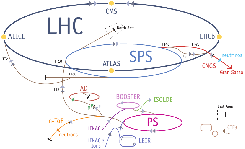
\includegraphics[width=.9\linewidth]{lhc_inj_chain}
    \caption{The LHC injection chain~\cite{LHCFAQ}.}
    \label{fig:lhc_inj_chain}
\end{figure}
%%% Local Variables:
%%% mode: latex
%%% TeX-master: "../search_for_DM_LED_with_ATLAS"
%%% End:


\section{The ATLAS Detector}
\label{sec:atlas-detector}

\gls{atlas} is a multi purpose detector designed to be sensitive to a large
physics signatures (supersymmetry and dark matter, briefly introduced in
Section~\ref{sec:supersymmetry} and Section~\ref{sec:dark-matter}) and to fully
take advantage of the LHC potential. It is capable of identifying photons,
electrons, muons, taus, jets and missing energy,
Figure~\ref{fig:atlas_particles} shows a schematic view of the interaction of
the different kind of particles with the ATLAS sub-detectors while
Figure~\ref{fig:atlas_overview} shows the ATLAS detector with its subsystems. In
the following sections a brief overview of the various subsystems that allow
particle identification and reconstruction is presented.
\begin{figure}[!htb]
  \centering
    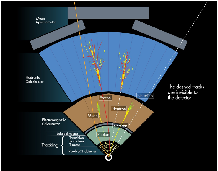
\includegraphics[width=.9\linewidth]{atlas_particles}
    \caption{Section of the ATLAS detector showing the interaction of different
      particle types with the sub-detectors~\cite{ATLASCrossSection}.}
    \label{fig:atlas_particles}
\end{figure}
\begin{figure}[!htb]
  \centering
    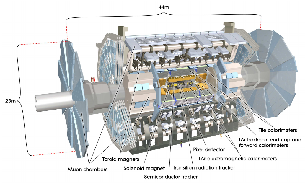
\includegraphics[width=.9\linewidth]{atlas_overview}
    \caption{Overview of the ATLAS detectors with its main
      sub-detectors~\cite{ATLASPaper}.}
    \label{fig:atlas_overview}
\end{figure}
%%% Local Variables:
%%% mode: latex
%%% TeX-master: "../search_for_DM_LED_with_ATLAS"
%%% End:


\subsection{The Coordinate System}
\label{sec:coordinate-system}

A right handed coordinate system is defined for the ATLAS detector, the origin
is at the geometric center of ATLAS with the $z$--axis oriented along the beam
direction and the $xy$ plane orthogonal to it. The positive $x$-axis points to
the center of the LHC ring while the positive $y$-axis is pointing upwards. The
A-side of the detector is defined as that with a positive $z$-axis while the
C-side has the negative $z$-axis.

The LHC beama are unpolarized and thus invariant under rotations around the beam
line axis, a cylindrical coordinate system is particularly convenient to
describe the detector geometry where:
\begin{equation}
  \label{eq:73}
  r = \sqrt{x^2 + y^2}, \quad \phi = \arctan \frac{y}{x}.
\end{equation}
A momentum dependent coordinate, the \emph{rapidity}, is commonly used in
particle physics for its invariance under Lorentz transformations along the
$z$--axis. The rapidity is defined as:
\begin{equation}
  \label{eq:74}
  y = \frac{1}{2} \ln \frac{E + p_z}{E - p_z}
\end{equation}
where $E$ is the energy of the particle and $p_z$ its momentum along the
$z$-axis. Rapidity intervals are Lorentz invariant under boost along the
$z$--axis. In the relativistic limit or when the mass of the particle is
negligible, the rapidity only depends on the production angle of the particle
with respect to the beam axis,
\begin{equation}
  \label{eq:75}
  \theta = \arctan \frac{\sqrt{p_x^2 + p_y^2}}{p_z}.
\end{equation}
This approximation is called \gls{eta} and is defined as:
\begin{equation}
  \label{eq:76}
  y \xrightarrow{p \gg m} \eta = - \ln \left( \tan \frac{\theta}{2} \right).
\end{equation}
A value of $\theta = 90^{\circ}$, perpendicular to the beam axis, corresponds to
$\eta = 0$. The spatial separation between particles in the detector is commonly
given in terms of a Lorentz invariant variable defined as:
\begin{equation}
  \label{eq:77}
  \Delta R = \sqrt{\Delta \phi^2 + \Delta \eta^2}.
\end{equation}

Other quantities used to describe the kinematics of the $pp$ interaction are the
\gls{pt} and the \gls{et} defined as $\pt = p \sin \theta$ and
$\et = E \sin \theta$ respectively.
%%% Local Variables:
%%% mode: latex
%%% TeX-master: "../search_for_DM_LED_with_ATLAS"
%%% End:


\subsection{The Inner Detector}
\label{sec:inner-detector}

The \gls{id}~\cite{ATLASPaper} is designed to provide good track reconstruction,
precise momentum resolution and both primary and secondary vertex measurements
(see Section~\ref{sec:primary-vertex}) above a nominal $\pt$ threshold of
0.5~GeV and within the pseudorapidity $|\eta| < 2.5$. The ID is 6.2~m long and
has a radius of about 1.1~m, it is surrounded by a solenoidal magnetic field of
2~T. Its layout is schematized in Figure~\ref{fig:id} and, as can be seen, it is
composed of three sub-detectors.

At the inner radius the \emph{pixel detector} measures charged particles with
silicon sensors with a minimum and maximum size of $50 \times 400$~$\mu$m$^2$
and $50 \times 600$~$\mu$m$^2$ respectively.

In the middle of the ID the \gls{sct} is designed to give eight precision
measurements per track which contribute to determine the primary and secondary
vertex position and momentum measurements. The silicon sensors are 80~$\mu$m
pitch micro strips.

The last layer of the ID is the \gls{trt}, it contributes to tracking and
identification of charged particles. It consists of drift (straw) tubes, 4~mm in
diameter with a 31~$\mu$m wire in the center of each straw, filled with a gas
mixture. These tubes substantially act like proportional counters where the tube
is the cathode and the wire is the anode and set to ground. When a charged
particle cross one tube, leaves a signal; the set of signals in the tubes,
reconstructs to a track which represents the path of the crossing object. The
space between the straw tubes is filled with material with a different
dielectric constant than the inside, this causes charged particles crossing the
boundaries to emit transition radiation thus leading to some straw to have a
much stronger signal. The transition radiation depends on the Lorentz $\gamma$
factor which in turn depends on the energy and the mass of the particles.
Lighter particles will have higher transition energy and stronger signal in the
straw tubes. This allows to distinguish between electrons (the lightest charged
particle) and single hadrons (pions), for instance, tracks with several strong
signal straw, can be identified as belonging to electrons.

An additional layer, the \gls{ibl}, was recently added in the region between the
beam pipe and the inner pixel layer (B-layer). It is designed to increase the
tracking robustness by replacing damaged parts of the pixel B-layer and
increasing the hit redundancy with higher luminosity. In addition, being closer
to the beam pipe it increases the impact parameter measurement
precision~\cite{IBL}.

\begin{figure}[!h]
  \centering
    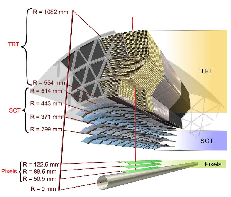
\includegraphics[width=.8\linewidth]{inner_detector}
    \caption{Schematic view of a charged track of 10~GeV $\pt$ that traverses
      the different ID sub-detectors. After traversing the beryllium pipe, the
      track passes through the three cylindrical silicon-pixel layers, the four
      layers of silicon-microstrip sensors (SCT) and the approximately 36 straws
      contained in the TRT within their support structure~\cite{ATLASPaper}.}
    \label{fig:id}
\end{figure}
%%% Local Variables:
%%% mode: latex
%%% TeX-master: "../search_for_DM_LED_with_ATLAS"
%%% End:


\subsection{The Calorimeter}
\label{sec:calorimeters}

The main purpose of a calorimeter is to measure the energy of electrons, photons
and hadrons by mean of materials capable of completely absorbing the energy of
the incoming particles transforming it in some measurable quantity. Calorimeters
can be classified in two categories, \gls{em} and \emph{hadronic} depending on
the particle they are designed to detect. The EM calorimeters are used to detect
photons and electrons while the task of hadronic calorimeters is to identify
hadrons. Both types of calorimeters can be further divided into \emph{sampling
  calorimeters} and \emph{homogeneous calorimeters}. Sampling calorimeters
alternate layers of a dense material used to absorb the energy of incident
particles (absorber) and an active material to collect the signal. The
interaction between the particles and the absorber produces a shower of
secondary particles with progressively degraded energy which is deposited in the
active material in form of charge or light that can be converted into
energy. Homogeneous calorimeters use only one material that serves both as an
absorber and an active material~\cite{Calorimetry}.

The ATLAS calorimeter is a sampling calorimeter covering up the $|\eta| < 4.9$
region the large $\eta$ coverage, ensures a good missing transverse momentum
measurement (see \cref{sec:miss-transv-energy}); an illustration of the system
is shown in \cref{fig:calo}.
\begin{figure}[!htb]
  \centering
    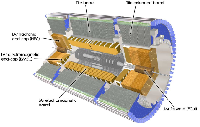
\includegraphics[width=.8\linewidth]{calorimeters}
    \caption{Cut-away view of the ATLAS calorimeter system~\cite{ATLASPaper}.}
    \label{fig:calo}
\end{figure}

The EM calorimeter has a barrel and two end-caps, covering the $|\eta| < 1.475$
and $1.375 < |\eta| < 3.2$ region respectively. It uses \gls{lar} as active
material and lead as absorber in an accordion geometry that provides $\phi$
symmetry without azimuthal cracks. In the region $|\eta| < 1.8$ a presampler
consisting of a LAr active region is used to correct for electrons and photons
energy loss upstream of the calorimeter.

There are three hadronic calorimeters: the \gls{tilecal}, the \gls{hec} and the
\gls{fcal}. The TileCal barrel and extended barrels cover the $|\eta| < 1.0$ and
$0.8 < |\eta| < 1.7$ and uses steel as absorber and scintillating tiles
connected to photomultipliers tubes through wavelength shifting fibers for
readout as an active material. The HEC covers the $1.5 < |\eta| < 3.2$ region
and, to avoid drops in material density at the transition, it overlaps slightly
with the FCal that covers the $3.1 < |\eta| < 4.9$.
%%% Local Variables:
%%% mode: latex
%%% TeX-master: "../search_for_DM_LED_with_ATLAS"
%%% End:


\subsection{The Muon Spectrometer}
\label{sec:muon-spectrometer}

The \gls{ms} is designed to identify muons and measure their momentum. It is
divided in four sub-detectors, the \gls{mdt}, the \gls{csc}, the \gls{rpc}, and
the \gls{tgc}. The sub-detectors are immersed in a magnetic field generated by
three different toroidal magnets, a barrel toroid covering the $|\eta| < 1.4$
region and two end-caps magnets at $1.6 < |\eta| < 2.7$, which produces a field
almost perpendicular to the muon tracks.

The MDT covers the $|\eta| < 2.7$ region and provides a precise measurement of
the track coordinates in the principal bending direction of the magnetic
field. It uses drift tubes to reconstruct the muon trajectory and the drift time
of the ionized charges is used to determine the minimum distance between the
wire and the muon. The CSC covers the $2.0 < |\eta| < 2.7$ region and is a
multi-wire proportional chamber with cathodes segmented in strips, one
perpendicular to the anode wire, providing the precision coordinate, and the
other parallel to it (giving the transverse coordinate).


The RPC and the TGC cover the $|\eta| < 1.05$ and $1.05 < |\eta| < 2.7$ regions
respectively. They contribute to the Level 1 trigger providing bunch crossing
identification, it allows to select high and low $\pt$ tracks and measure the
muon coordinate in the direction orthogonal to that determined by MDT and CSC\@.

\begin{figure}[!h]
  \centering
    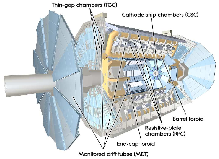
\includegraphics[width=.7\linewidth]{muon_spectro}
    \caption{Cut-away view of the ATLAS muon spectrometer~\cite{ATLASPaper}.}
    \label{fig:muon_spectro}
\end{figure}
%%% Local Variables:
%%% mode: latex
%%% TeX-master: "../search_for_DM_LED_with_ATLAS"
%%% End:


\subsection{The Forward Detectors}
\label{sec:forward-detectors}

The ATLAS forward region is covered by three smaller detectors: the \gls{lucid},
the \gls{alfa} and the \gls{zdc}. LUCID~\cite{ForwardDetectors} is located at
$\pm 17$~m from the IP, it is designed to monitor the relative luminosity by
detecting the inelastic $pp$ scattering. The ZDC~\cite{ForwardDetectors} is
located at $\pm 140$~m from the IP, it consists of alternating layers of quartz
rods and tungsten plates designed to measure neutron at $|\eta| < 8.2$, its
purpose is to measure the centrality in heavy-ion
collisions. ALFA~\cite{ForwardDetectors} is located at $\pm 240$~m from the IP
and is designed to measure the absolute luminosity via elastic scattering at
small angles.
%%% Local Variables:
%%% mode: latex
%%% TeX-master: "../search_for_DM_LED_with_ATLAS"
%%% End:


\subsection{The Trigger System}
\label{sec:trigger-system}

The bunch crossing rate at LHC is 40~MHz for a bunch spacing of 25~ns (about 7
meters). Each event recorded by ATLAS requires $\approx 1.4$~MB of disk space,
with approximately 20 to 50 collisions per bunch crossing, the storage space
required to record all the events in a second would be $\approx 60$~TB. This is
not feasible thus only the most interesting events are selected and stored on
disk. The \emph{trigger system} decides whether to keep or not a collision event
for later studies, it consists of a hardware based \gls{l1} trigger and a
software based \gls{hlt}.

The L1 trigger determines \gls{rois} in the detector using custom hardware and
coarse information from the calorimeter and the muon system. The L1 trigger is
capable of reducing the event rate to 100~kHz with a decision time for a L1
accept of 2.5~$\mu$s. The RoIs from the L1 trigger are sent to the HLT where
different algorithms are run using the full detector information and reducing
the L1 output rate to 1~kHz with a processing time of about
200~ms~\cite{trigger}. %A schematic overview of the ATLAS trigger and data
%acquisition system is shown in Figure~\ref{fig:trigger_system}.

In the monojet analysis presented in this thesis, the HLT\_xe70 trigger is used,
it receives an L1 accept that selects events with a missing energy (see
Section~\ref{sec:miss-transv-energy}) greater than 50~GeV, no muons are used in
the reconstruction of the missing energy at the trigger level. The events that
survive L1 are then passed to the HLT level, where events with a missing energy
greater than 70~GeV are selected.
% \begin{figure}[!h]
%   \centering
%     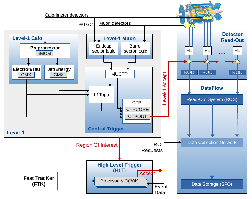
\includegraphics[width=.7\linewidth]{trigger_system}
%     \caption{Schematic view of the ATLAS trigger and data acquisition system.}
%     \label{fig:trigger_system}
% \end{figure}
%%% Local Variables:
%%% mode: latex
%%% TeX-master: "../search_for_DM_LED_with_ATLAS"
%%% End:


\chapter{Noise Studies with the Tile Calorimeter}
\label{cha:noise-studies-with}

\section{Calorimetry}
\label{sec:calorimetry}

Particles lose energy interacting with matter. The particle's energy and its
type determines the processes causing the energy loss; these can be of two kind,
\emph{electromagnetic} and \emph{hadronic}. In this section a brief overview of
the physics behind these interactions is given.
%%% Local Variables:
%%% mode: latex
%%% TeX-master: "../search_for_DM_LED_with_ATLAS"
%%% End:


\subsection{Electromagnetic Shower}
\label{sec:electr-show}

High energy electrons and photons lose energy mainly by \emph{radiation} and
\emph{conversion} respectively. When electrons with energies greater than
$\sim 10$~MeV interact with the electromagnetic field of the absorber nuclei
\emph{Bremsstrahlung} can occur. High energy photons produce mostly
electron--positron pairs.

Electrons and photons with a sufficient amount of energy interacting with an
absorber, produce secondary photons through Bremsstrahlung or secondary
electrons and positrons by pair production. These secondary particles will
produce more particles through the same mechanisms giving rise to a shower of
particles with progressively lower energies. When the energy loss in the shower
is dominated by ionization and thermal excitation of the active material atoms,
the number of particles in the shower stops growing and there is no further
shower development. The above process goes on until the energy of the electrons
falls below a critical energy, $\epsilon$, where ionization and excitation
becomes the dominant effects~\cite{Calorimetry}.
%%% Local Variables:
%%% mode: latex
%%% TeX-master: "../search_for_DM_LED_with_ATLAS"
%%% End:


\subsection{Hadronic Shower}
\label{sec:hadronic-shower}

Hadrons lose energy through strong interaction with the calorimeter
material. The strong interaction is responsible for the production of energetic
secondary hadrons with momenta typically at the GeV scale and nuclear reactions
such as excitation or nucleon spallation in which neutrons and protons are
released from the nuclei with a characteristic energy at the MeV scale.

These energetic hadrons are protons, neutrons and pions. On average, 1/3 of the
pion produced are neutral pions which decay to photons
($\pi \rightarrow \gamma \gamma$). The photons produced this way will initiate
an electromagnetic shower as described in Section~\ref{sec:electr-show}
transferring energy from the hadronic part to the electromagnetic shower inside
the hadronic shower. The electromagnetic component of the shower does not
contribute any more to hadronic processes. The nucleons released by excitation
or nuclear spallation, require an energy equal to their binding energy to be
released and are not recorded as a contribution to the calorimeter signal thus
producing a form of \emph{invisible energy}. Some detectors can compensate for
the loss of invisible energy, these are called \emph{compensating
  calorimeters}~\cite{Calorimetry}.
%%% Local Variables:
%%% mode: latex
%%% TeX-master: "../search_for_DM_LED_with_ATLAS"
%%% End:


\subsection{Energy Resolution}
\label{sec:energy-resolution}

The energy resolution of a detector measures its ability of distinguishing
between particles of different energies; the better the energy resolution, the
better it can separate energy peaks belonging to different decays.

The energy resolution can be written as:
\begin{equation}
  \label{eq:64}
  \frac{\sigma_E}{E} = \frac{a}{\sqrt{E}} \oplus \frac{b}{E} \oplus c,
\end{equation}
where the $\oplus$ symbol indicates a quadratic sum. The first term ($a$) in the
equation is the \emph{stocastic term}, it is mainly due to fluctuations related
to the physical evolution of the shower. In homogeneous calorimeters, this term
is small because the energy deposited in the active volume by a monochromatic
beam of particles is constant for each event. In a sampling calorimeter, the
active layers are interleaved with absorber layers thus the energy deposited in
the active material fluctuates event by event. These are called \emph{sampling
  fluctuations} and, in sampling electromagnetic calorimeters, represents the
greatest limitation to energy resolution due to the variation in the number of
charged particles which cross the active layers. The second term ($b$) in
eq.~\eqref{eq:64} is called the \emph{noise term}, it comes from the electronic
noise of the detector readout chain. Sampling or homogeneous calorimeters which
collect the signal in the form of light, using for example a photo-multiplier
tube with a high gain multiplication of the signal with a low electronic noise,
can achieve low levels of noise. Calorimeters that collect the signal in form of
charge, must use an pre-amplifier having thus a higher level of noise. In
sampling calorimeters, the noise term can be further reduced by increasing the
sampling fraction, this way there is a larger signal coming from the active
material and a higher noise--to--signal ratio. The last term ($c$) of the
equation is the \emph{constant term}, it does not depend on the energy of the
particles but includes all the non uniformities in the detector response such as
instrumental effect, imperfections in the calibration of different parts of the
detector, radiation damage, detector aging, or the detector
geometry~\cite{Calorimetry}.
%%% Local Variables:
%%% mode: latex
%%% TeX-master: "../search_for_DM_LED_with_ATLAS"
%%% End:


\section{The ATLAS TileCal}
\label{sec:atlas-tilecal}

TileCal is the central hadronic calorimeter of the ATLAS experiment covering the
$|\eta| < 1.7$ region. It is designed for energy measurement of hadrons, jets,
tau particles and also contributes to the measurement of missing transverse
energy (see Section~\ref{sec:miss-transv-energy}). TileCal is a scintillator
steel non compensating sampling calorimeter, the scintillation light produced in
the tiles is transmitted by \glspl{wsf} to \glspl{pmt}. The analog signals from
the PMTs are amplified, shaped and digitized by sampling the signal every
25~ns. The TileCal front end electronics read out the signals produced by about
10000 channels measuring energies ranging from 30~MeV to 2~TeV. The readout
system is responsible for reconstructing the data in real time. The digitized
signals are reconstructed with the Optimal Filtering algorithm (see
Section~\ref{sec:optimal-filtering}), which computes for each channel the signal
amplitude, time and quality factor at the required high rate.

TileCal is designed as one \gls{lb} covering the $|\eta| < 1.0$ range and two
\gls{eb} in the $0.8 < |\eta| < 1.7$ range. The barrels are further divided,
according to their geometrical position on the $z$-axis, in partitions called
EBA, LBA, EBC and LBC (see Section~\ref{sec:coordinate-system}). Each partition
consists of 64 independent wedges (see Figure~\ref{fig:tile_mod}) called
\emph{modules} assembled in azhimut ($\phi$). The LBA and EBA partitions are
shown in Figure~\ref{fig:tile_cells}.

\begin{figure}[!h]
  \centering
    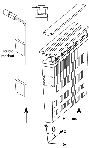
\includegraphics[width=.5\linewidth]{tile_module}
    \caption{Cut away showing an individual TileCal module along with the
      optical read out and design of a TileCal module~\cite{TileModule}.}
    \label{fig:tile_mod}
\end{figure}

Between the LB and the EB there is a 600~mm gap needed for the ID and the LAr
cables, electronics and services. Part of the gap contains the \gls{itc}, a
detector designed to maximize the active material while leaving enough space for
services and cables. The ITC is an extension of the EB and it occupies the 0.8 <
$|\eta|$ < 1.6 region. The combined 0.8 < $|\eta|$ < 1.0 part is called
\emph{plug} and in the 1.0 < $|\eta|$ < 1.6 region, for space reasons, the ITC
is not interleaved with an absorber and is only composed of scintillator
material. The scintillators between 1.0 < $|\eta|$ < 1.2 are called \emph{gap
  scintillators}, while those between 1.2 < $|\eta|$ < 1.6 are called
\emph{crack scintillators}. The plug and the gap scintillators mainly provide
hadronic shower sampling while the crack scintillator, which extends to the
region between the barrel and the end-cap cryostats, samples the electromagnetic
shower in a region where the normal sampling is impossible due to the dead
material of the cryostat walls and the ID cables.

TileCal is also divided in longitudinal layers, the A, BC and D layers as shown
in \cref{fig:tile_cells}. The two innermost layers have a
$\Delta \eta \times \Delta \phi$ segmentation of $0.1 \times 0.1$ while in the
outermost, the segmentation is $0.1 \times 0.2$. Each layer is logically divided
into \emph{cells} (also shown in \cref{fig:tile_cells}) by grouping together in
the same PMT the fibers coming from different scintillator tiles belonging to
the same radial depth. The gap/crack scintillators are also called E layer
cells.

The energy resolution for jets in ATLAS is:
\begin{equation}
  \label{eq:65}
  \frac{\sigma_E}{E} = \frac{50\%}{\sqrt{E}} \oplus 3\%
\end{equation}
for $|\eta| < 3$. The 3\% constant term becomes dominant for high energy hadrons
where an increase in energy resolution is expected~\cite{TileCal}.

\begin{figure}[!h]
  \centering
    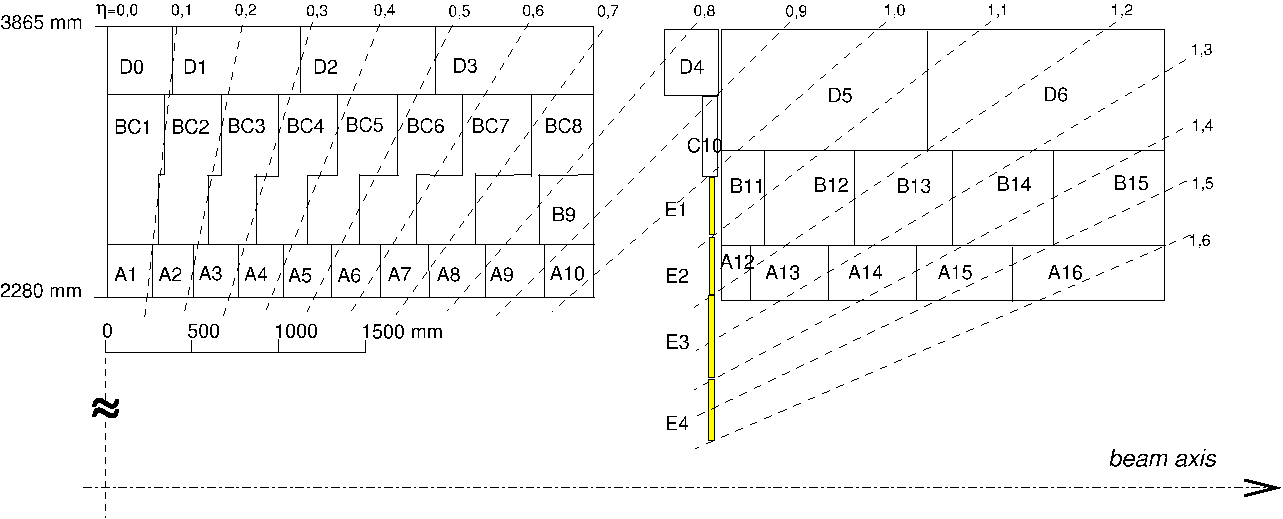
\includegraphics[width=\linewidth]{tile_cells}
    \caption{Schematic view of the TileCal layer and cell structure in a plane
      containing the beam axis $z$~\cite{TileCalPub}.}
    \label{fig:tile_cells}
\end{figure}
%%% Local Variables:
%%% mode: latex
%%% TeX-master: "../search_for_DM_LED_with_ATLAS"
%%% End:


\subsection{Signal Reconstruction}
\label{sec:sign-reconstr}

The TileCal cells are read out by two PMTs with the exception of the E layer
cells that are connected to only one photomultiplier tube using \gls{wsf}. Each
PMT is associated to an electronic read--out channel with its own shaper,
preamplifier and \gls{adc}. The current pulse from the PMTs is shaped and
amplified by the 3--in--1 card. There are two possible gains: \gls{hg} and
\gls{lg}, with an amplification ratio of 64. The 3-in-1 card forms the front-end
electronics of the read-out chain and provides three basic functions: shaping of
the pulse, charge injection calibration and slow integration of the PMT signals
for monitoring and calibration~\cite{TileCal}. Up to twelve 3--in--1 cards are
serviced by a motherboard that provides power and individual control signals.
The amplified signal is sent to two \glspl{adc} synchronous with the 40~MHz LHC
clock thus sampling the signal every 25~ns. For optimization and efficiency
reasons, 7 samples for each pulse are taken and sent to the \glspl{rod} if an L1
trigger accept is received.
%%% Local Variables:
%%% mode: latex
%%% TeX-master: "../search_for_DM_LED_with_ATLAS"
%%% End:


\subsubsection{Optimal Filtering}
\label{sec:optimal-filtering}

The seven samples are used to reconstruct the amplitude of the pulse using the
\gls{of} method. The estimate of the amplitude is given by:
\begin{equation}
  \label{eq:66}
  \hat{A} = \sum_{i = 0}^7 a_i S_i
\end{equation}
where $S_i$ are the digitized samples expressed in ADC counts and $a_i$ are
computed weights that minimize the effect of the electronic noise on the
amplitude reconstruction. The procedure minimizes the variance of the amplitude
distribution. In order to make the amplitude reconstruction independent from
phase and signal baseline due to electronic noise (\emph{pedestal}), the
following constraints are used:
\begin{equation}
  \label{eq:67}
  \sum_{i = 0}^7 g_i a_i = 0
\end{equation}
\begin{equation}
  \label{eq:68}
  \sum_{i = 0}^7 g'_i a_i = 0
\end{equation}
\begin{equation}
  \label{eq:69}
  \sum_{i = 0}^7 a_i = 0
\end{equation}
where $g_i$ and $g'_i$ are the pulse shape function from the shaper and its
derivative~\cite{OptimalFilter}.
%%% Local Variables:
%%% mode: latex
%%% TeX-master: "../search_for_DM_LED_with_ATLAS"
%%% End:


\subsubsection{The TileCal Calibration}
\label{sec:tilecal-calibration}

The energy deposited in the calorimeter cell is proportional to the
reconstructed amplitude. The amplitude is originally measured in ADC counts and
needs to be converted in GeV for physics analysis using the formula:
\begin{equation}
  \label{eq:70}
  E[GeV] = \hat{A}[ADC] \times C_{ADC \rightarrow pC} \times C_{\text{laser}}
  \times C_{Cs} \times C_{pC \rightarrow GeV}
\end{equation}
where $\hat{A}[ADC]$ is the amplitude estimate in ADC counts, $C_{ADC \rightarrow
pC}$ is determined using the \gls{cis}, $C_{pC \rightarrow
  GeV}$ is measured during testbeam using electrons with a well defined energy
and converts the deposited charge to energy in GeV, the laser system allows to
determine the value of the $C_{\text{laser}}$ constant while the Cesium sets the
$C_{Cs}$ factor.

The CIS calibrates the read out electronics by injecting a known charge and
measuring the resulting response of the electronics. The \emph{laser} system
main purpose is to monitor the photomultipliers tubes stability and the
downstream electronics. Well calibrated light pulses are sent to the PMTs and by
reconstructing the signal it is possible to extract the PMTs' gain. The
\emph{cesium} system, circulates a Cs source through each scintillating tile
using an hydraulic system, the PMTs signal is continuously read out through an
integrator. The cesium system allows to equalize the calorimeter cell response
to that measured during test beams. Figure~\ref{fig:cali_chain} depicts a
schematic representation of the ATLAS TileCal calibration chain.

\begin{figure}[!h]
  \centering
    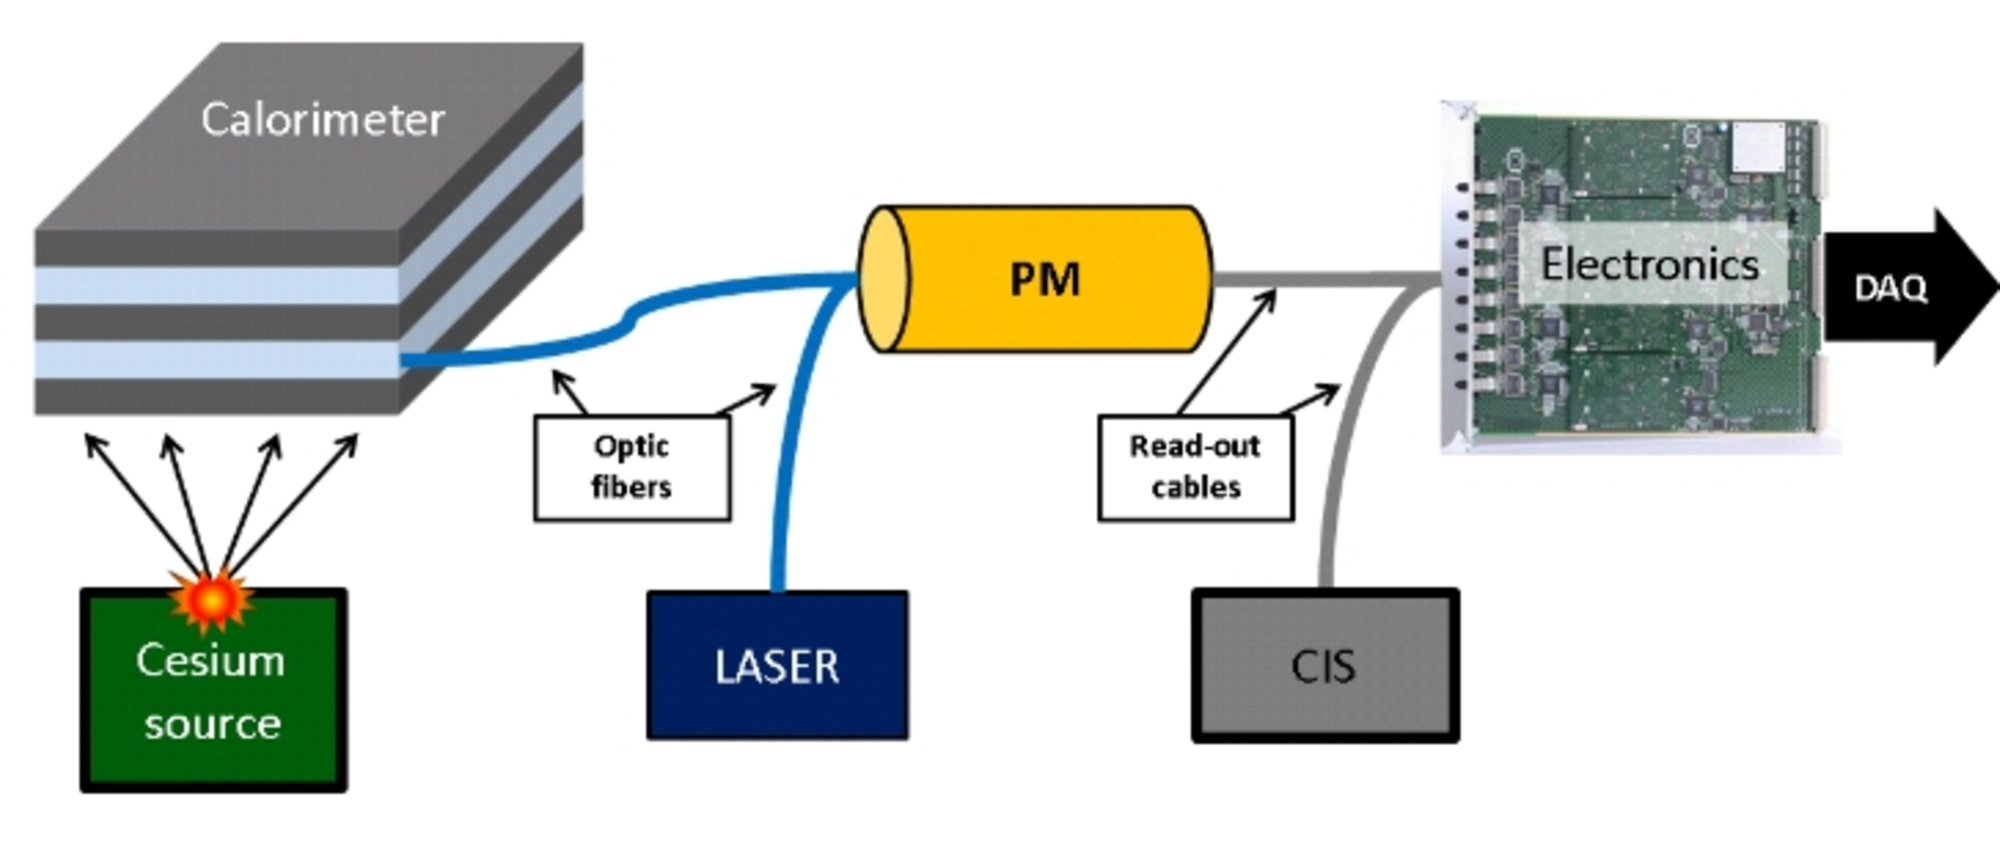
\includegraphics[width=.8\linewidth]{calibration_chain}
    \caption{The ATLAS TileCal calibration chain~\cite{TileCalibChain}.}
    \label{fig:cali_chain}
\end{figure}
%%% Local Variables:
%%% mode: latex
%%% TeX-master: "../search_for_DM_LED_with_ATLAS"
%%% End:


\subsection{Electronic Noise}
\label{sec:electronic-noise}

TileCal periodically records sets of events (referred to as \emph{runs}) with no
signal in the PMTs, called \emph{pedestal runs}. During these runs, each channel
is read out using both, HG and LG for about 100000 events. These events are
sampled every 25~ns in 7 samples as in normal physics runs and are normally
distributed around a mean value called \emph{pedestal}. The \gls{rms} of the
pedestal is the \emph{noise}. Pedestal runs are used to calculate different
parameters called \emph{noise constants} that allow to describe the electronic
noise. Two different sets of noise constants are computed: \emph{Digital Noise}
(or \emph{Sample Noise}) and \emph{Cell Noise}.
%%% Local Variables:
%%% mode: latex
%%% TeX-master: "../search_for_DM_LED_with_ATLAS"
%%% End:


\subsubsection{Digital Noise}
\label{sec:digital-noise}

The digital noise is measured in ADC counts for each PMT in both gains, HG and
LG\@. The noise constants together with all detector conditions are stored in
the \gls{cool}. These constants are the RMS of the seven samples within each
event, also called \gls{hfn} and the RMS of the first digitized sample in each
event or \gls{lfn}. The digital noise is used for monitoring the electronics and
for \gls{mc} noise simulation of the calorimeter response.
%%% Local Variables:
%%% mode: latex
%%% TeX-master: "../search_for_DM_LED_with_ATLAS"
%%% End:


\subsubsection{Cell Noise}
\label{sec:cell-noise}

Excluding the E layer cells that are connected only to one PMT, the cell noise
is the combination of the two readout channels of a cell where the digital noise
from the PMTs is added quadratically and converted in MeV using the calibration
constants and \cref{eq:84}. There are four possible gain combinations:
\gls{hghg}, \gls{lglg}, \gls{lghg} and \gls{hglg}. When the energy deposit is
large, the two channels belonging to the cell are readout in low gain thus
giving rise to the LGLG combination, for small signals the HGHG combination is
used. It can also occur that for energy deposits in the intermediate range, one
PMT is readout in LG and the other in HG resulting in a HGLG combination. The
cell noise is used to identify the seed cells in the topocluster algorithm (see
Section~\ref{sec:topocluster}).

Figure~\ref{fig:non_gaussianity} shows a comparison between the cell noise and
the fitted $\sigma$ parameter of a normal distribution. The ratio RMS / $\sigma$
= 1 indicates a perfect agreement between the measured and the fitted amplitude
distribution for a single Gaussian hypothesis. The blue square in the plot
indicate the comparison for an old model of \gls{lvps} while the red square
refers to the currently used LVPSs. It can be seen that with the old model of
\glspl{lvps} the ratio RMS / $\sigma$ can be large indicating a non Gaussian
behavior of the electronic noise. For this reason a double Gaussian distribution
is used to fit the energy distribution with the probability density function
defined as:
\begin{equation}
  \label{eq:85}
  f_{2g} = \frac{1}{1 + R} \left( \frac{1}{\sqrt{2 \pi} \sigma_1} e^{-
      \frac{x^2}{2 \sigma_1^2}} + \frac{R}{\sqrt{2 \pi} \sigma_2} e^{-
      \frac{x^2}{2 \sigma_2^2}} \right)
\end{equation}
where $R$ is the relative normalization of the two Gaussians and
$\sigma_1, \sigma_2$ and $R$ are independent parameters. These three are used to
define the region $\sigma_{\text{eff}}(E)$ where the significance for the double
Gaussian is the same as the one $\sigma$ region for a single Gaussian,
i.e.
$\int_{- \sigma_{\text{eff}}}^{\sigma_{\text{eff}}} f_{2g} =
0.68$~\cite{TileReadiness}.
In terms of $\sigma_{\text{eff}}$, for an energy deposit $E$, the significance
can be expressed as:
\begin{equation}
  \label{eq:86}
  \frac{E}{\sigma_{\text{eff}}(E)} = \sqrt{2}\ \text{Erf}^{- 1} \left( \frac{\sigma_1
      \text{Erf} \left(\frac{E}{\sqrt{2 \sigma_1}} \right) + R \sigma_2 \text{Erf}
    \left( \frac{E}{\sqrt{2 \sigma_2}} \right)}{\sigma_1 + R \sigma_2} \right)
\end{equation}
where Erf is the error function. Equation~\ref{eq:86} is the input to the
calorimeter cell clustering algorithm discussed in more details in
\cref{sec:topocluster}, moreover this definition allows to use the same unit to
describe the noise for both the TileCal and LAr calorimeters. The region
$\sigma_{\text{eff}}(E)$ is commonly referred to as \emph{cell noise} and
together with the three double Gaussian parameters ($\sigma_1$, $\sigma_2$ and
R) is stored in the COOL database.

\begin{figure}[!h]
  \centering
    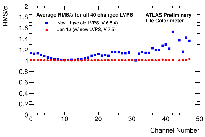
\includegraphics[width=.8\linewidth]{non_gaussianity}
    \caption{Comparison between the TileCal electronic noise, measured as the
      RMS of the reconstructed amplitude distribution in pedestal runs and the
      $\sigma$ of the Gaussian fit of the distribution for the old and new
      LVPS~\cite{TileCalNoisePub}.}
    \label{fig:non_gaussianity}
\end{figure}
%%% Local Variables:
%%% mode: latex
%%% TeX-master: "../search_for_DM_LED_with_ATLAS"
%%% End:


\section{The 2011 TileCal Run I Reprocessing}
\label{sec:2011-tilecal-run}

As new information about the detector becomes available, an update of the
calibration constants and thus of the reconstructed energy must be performed;
this procedure is called \emph{reprocessing}. In 2011 an update of the laser and
cesium calibration analysis procedure were performed together with an update of
which cells were considered good or bad. These updates required a recalculation
of the cell noise.
%%% Local Variables:
%%% mode: latex
%%% TeX-master: "../search_for_DM_LED_with_ATLAS"
%%% End:


\subsection{Results}
\label{sec:results-1}

The cell noise for the reprocessed data has been calculated in the different
gain combinations. In
\cref{fig:noise_avg_hghg,fig:noise_avg_lglg,fig:noise_avg_hglg} the cell noise
values have been calculated using all the calibration runs used for the 2011 RUN
I reprocessing, each fitted using the optimal filtering method (see
\cref{sec:optimal-filtering}). The plots show the $\eta$--dependence of the
$\phi$--averaged RMS of the noise in these runs. Each point is an average for a
given cell over all modules containing this cell type. This is done for a given
gain combination of the readout channels: High Gain--High Gain
(\cref{fig:noise_avg_hghg}), Low Gain--Low Gain (\cref{fig:noise_avg_lglg}) or
High Gain--Low Gain (\cref{fig:noise_avg_hglg}). The plots separate the
different cell types: A, BC, D and E (gap and crack scintillators). Note that
gap and crack scintillators have only one readout channel, so are plotted only
in HG or LG readout. The transition between the long and extended barrels can be
seen in the range $0.7 < |\eta| < 1.0$.
\begin{figure}[!h]
  \centering
    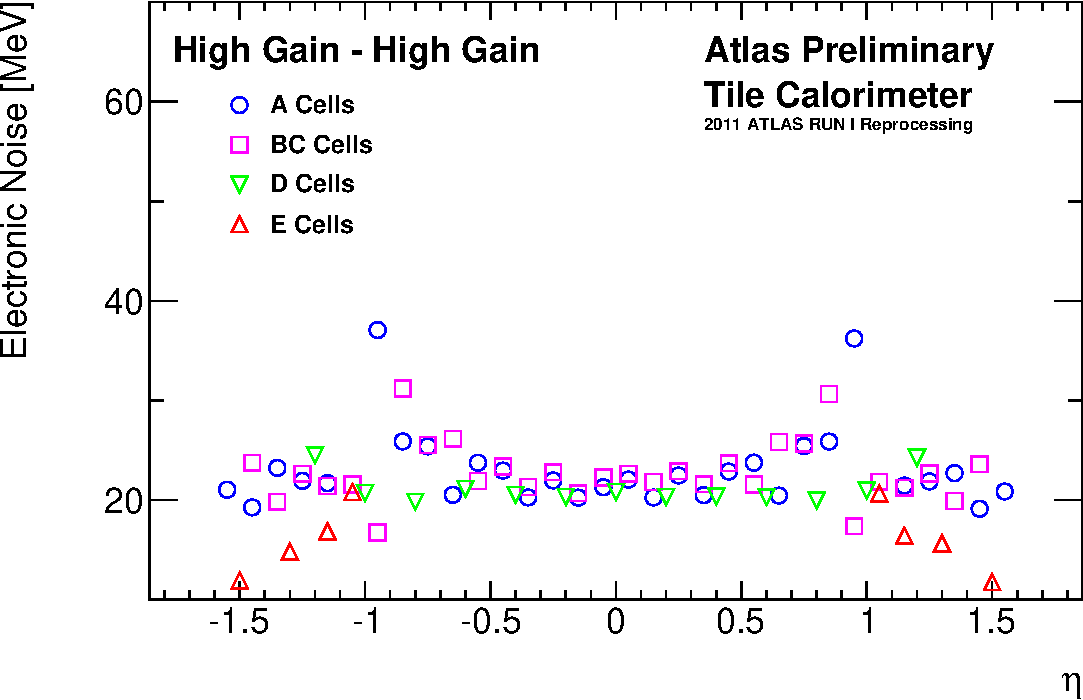
\includegraphics[width=.8\linewidth]{noise_avg_hghg}
    \caption{$\phi$--averaged RMS of electronic cell noise as a function of
      $\eta$ of the cell, with both readout channels in High Gain. For each cell
      the average value over all modules is taken. Values have been extracted
      using all the calibration runs used for the 2011 RUN I reprocessing. The
      different cell types are shown separately, A, BC, D, and E
      (gap/crack). The transition between the long and extended barrels can be
      seen in the range $0.7 < |\eta| < 1.0$. HGHG combination is relevant when
      the energy deposition in the cell is
      $\lesssim 15$~GeV~\cite{MyTileCalPlots}.}
    \label{fig:noise_avg_hghg}
\end{figure}

\begin{figure}[!h]
  \centering
    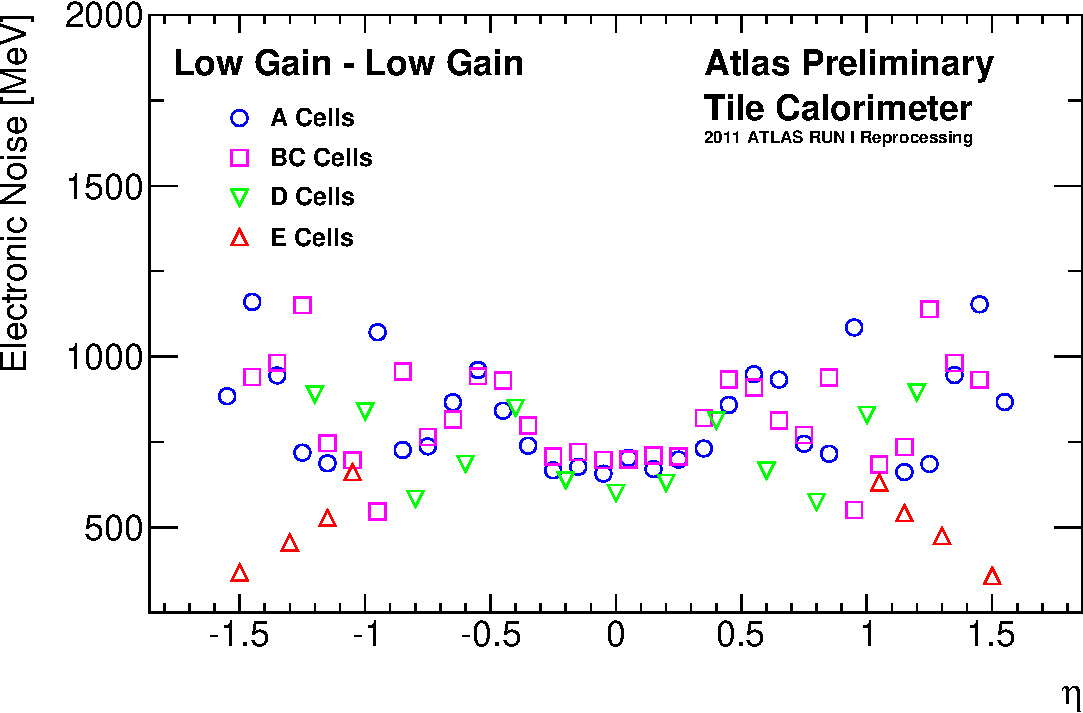
\includegraphics[width=.8\linewidth]{noise_avg_lglg}
    \caption{$\phi$-averaged RMS of electronic cell noise as a function of
      $\eta$ of the cell, with both readout channels in Low Gain. For each cell
      the average value over all modules is taken. Values have been extracted
      using all the calibration runs used for the 2011 RUN I reprocessing. The
      different cell types are shown separately, A, BC, D, and E
      (gap/crack). The transition between the long and extended barrels can be
      seen in the range $0.7 < |\eta| < 1.0$. LGLG combination is relevant when
      the energy deposition in the cell is
      $\gtrsim 15$~GeV~\cite{MyTileCalPlots}.}
    \label{fig:noise_avg_lglg}
\end{figure}

\begin{figure}[!h]
  \centering
    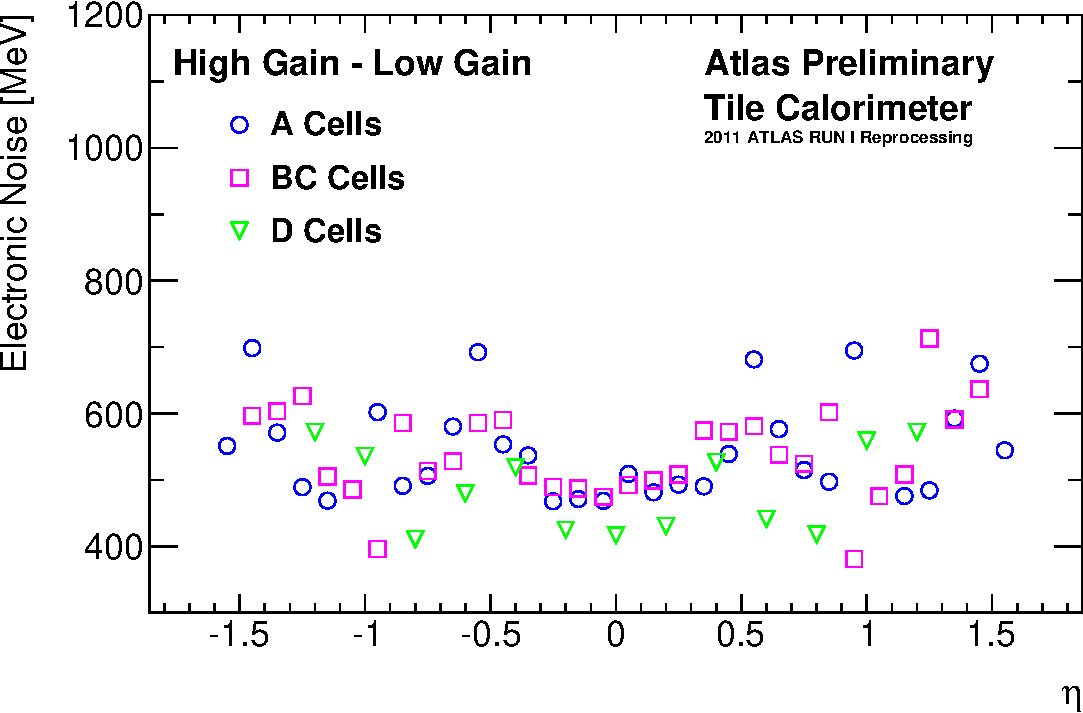
\includegraphics[width=.8\linewidth]{noise_avg_hglg}
    \caption{$\phi$-averaged RMS of electronic cell noise as a function of
      $\eta$ of the cell, with one readout channel in High Gain and the other in
      Low Gain. For each cell the average value over all modules is
      taken. Values have been extracted using all the calibration runs used for
      the 2011 RUN I reprocessing. The different cell types are shown
      separately, A, BC, D. E cells do not appear int this plot since they have
      only one readout channel. The transition between the long and extended
      barrels can be seen in the range $0.7 < |\eta| < 1.0$. When the energy
      deposition in the cell is between 10~GeV $\lesssim E \lesssim$ 20~GeV it
      can happen that the cell is read out with different voltage on the readout
      channels~\cite{MyTileCalPlots}.}
    \label{fig:noise_avg_hglg}
\end{figure}

\cref{fig:noise_avg_hghg,fig:noise_avg_lglg,fig:noise_avg_hglg} exhibit some
$\eta$--dependence of the noise. There are two main factors behind this, first
the low voltage power supplies, which are the main noise source in TileCal, are
located approximately at $|\eta| \approx 1$ leading to higher noise in the cells
in that region. Secondly the noise in these plots is in MeV, cells with the same
noise expressed in ADC counts can have different noise levels when converted in
MeV. This is due to the different ADC to GeV calibration factors for cells with
different geometries.
% Figures 5.5 to 5.exhibit some eta-dependence of the noise. There are two main
% factors behind this, first the low voltage power supplies are known to be the
% main source of noise in TileCal, they are located at |eta|~1 and lead to higher
% noise in the cells in that region.  Secondly the noise in these figures is shown
% in MeV. Two channels with the same noise expressed in ADC counts can have
% different noise levels expressed in MeV as two cells with different geometries
% will have different ADC to GeV calibration factors.
%%% Local Variables:
%%% mode: latex
%%% TeX-master: "../search_for_DM_LED_with_ATLAS"
%%% End:


\section{Time Stability}
\label{sec:time-stability}

The calibration constants used in \cref{eq:84}, as mentioned in
\cref{sec:tilecal-calibration}, are determined with the help of several
dedicated calibration systems and runs. Each calibration constant is valid over
a period of time called \gls{iov}. The cell noise can vary over time for several
reasons such as a change in the calibration constants, a variation in the
digital noise or the channel status in a particular run. Sudden variations in
the noise must be checked and understood.

The different TileCal subsystems (laser, CIS, etc.) all use a common software
framework, \gls{tucs}, to perform validity checks on a number of different
studies. To study the stability over time of the updated noise constants, a set
of python scripts was developed by the author of this thesis to expand the TUCS
functionality. These scripts connect to the ATLAS condition database and allow
to visually display the relative change of the cell noise and digital noise
constants, the channel status and the ratio between the cell noise and a
variable called RMS$_\text{eff}$ and defined as:
\begin{equation}
  \label{eq:87}
  \text{RMS}_{\text{eff}} = \sqrt{(1 - R) \sigma_1^2 + R \sigma_2^2}
\end{equation}
where $\sigma_1$, $\sigma_2$ and R are the free parameters in the double
Gaussian model (see Section~\ref{sec:cell-noise}). The ratio
$\sigma$~/~RMS$_\text{eff}$, where $\sigma$ is the cell noise, can be used to
test the goodness of the double Gaussian model: if $\sigma$~/~RMS$_\text{eff}$
equals one, the double Gaussian well models the noise, if
$\sigma$~/~RMS$_\text{eff}$ $> 1$, it means that there is noise that is not well
described by it.

\cref{fig:jumps} shows the time evolution plot over the entire reprocessed
period for two representative TileCal cells. This represents the typical
behavior for most cells over the reprocessing period.

In \cref{fig:no_jumps} it can be seen that cell number 2 in the BC layer (BC2)
of the 41st module in the C side of LB (LBC 41) is stable over several pedestal
runs. In Figure~\ref{fig:with_jumps} on the other hand, it is possible to see a
variation in the cell noise and of the $\sigma$~/~RMS$_{\text{eff}}$ without a
corresponding variation in the calibration, in the digital noise constants or in
the channel status. The term \emph{jump} is used in the following to indicate a
variation in the cell noise not compatible with a change in the other
quantities.
\begin{figure}[!ht]
  \centering
  \begin{subfigure}[t]{.95\linewidth}
    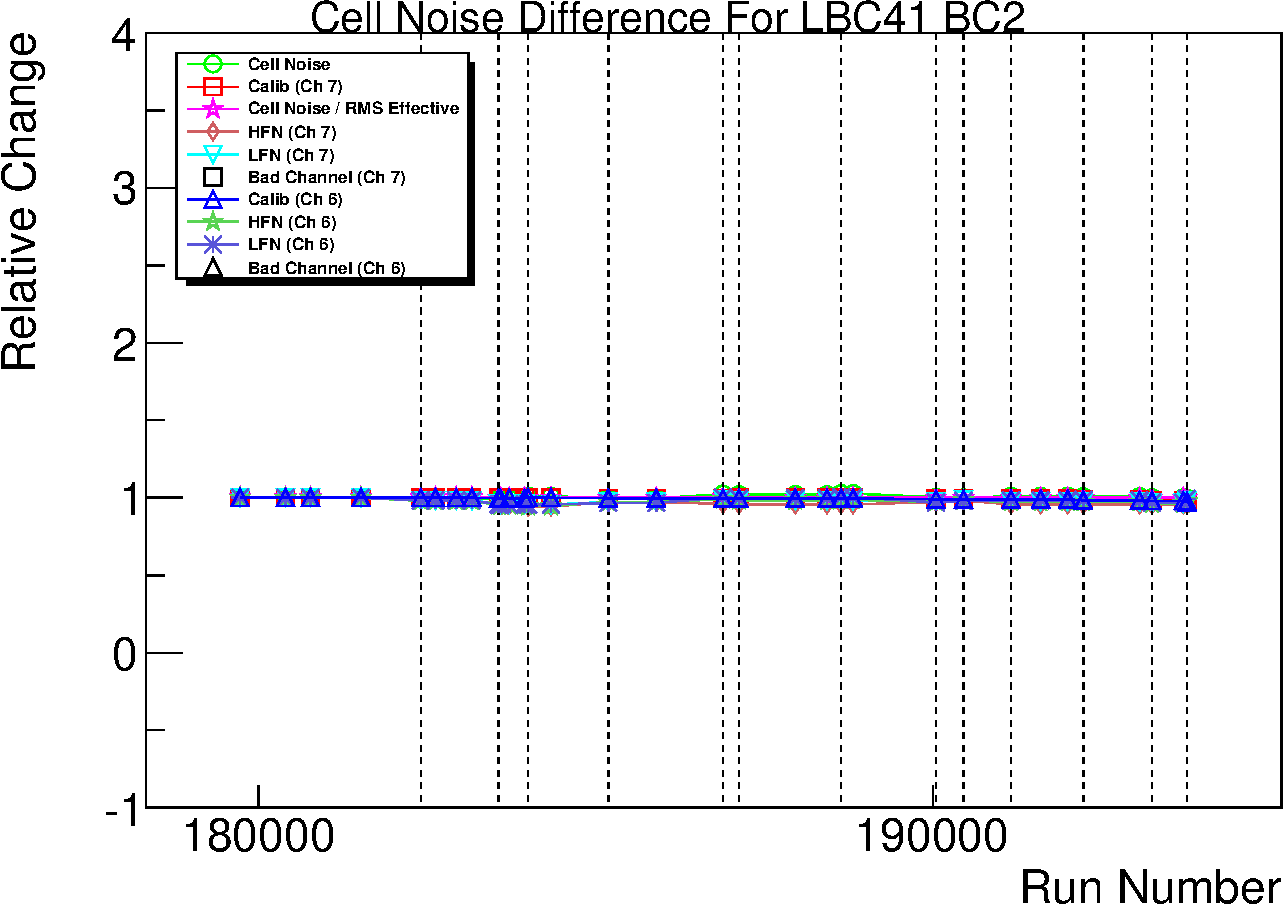
\includegraphics[width=\linewidth]{no_jumps}
    \caption{Control cell with no variation.}
    \label{fig:no_jumps}
  \end{subfigure}
  \begin{subfigure}[t]{.95\linewidth}
    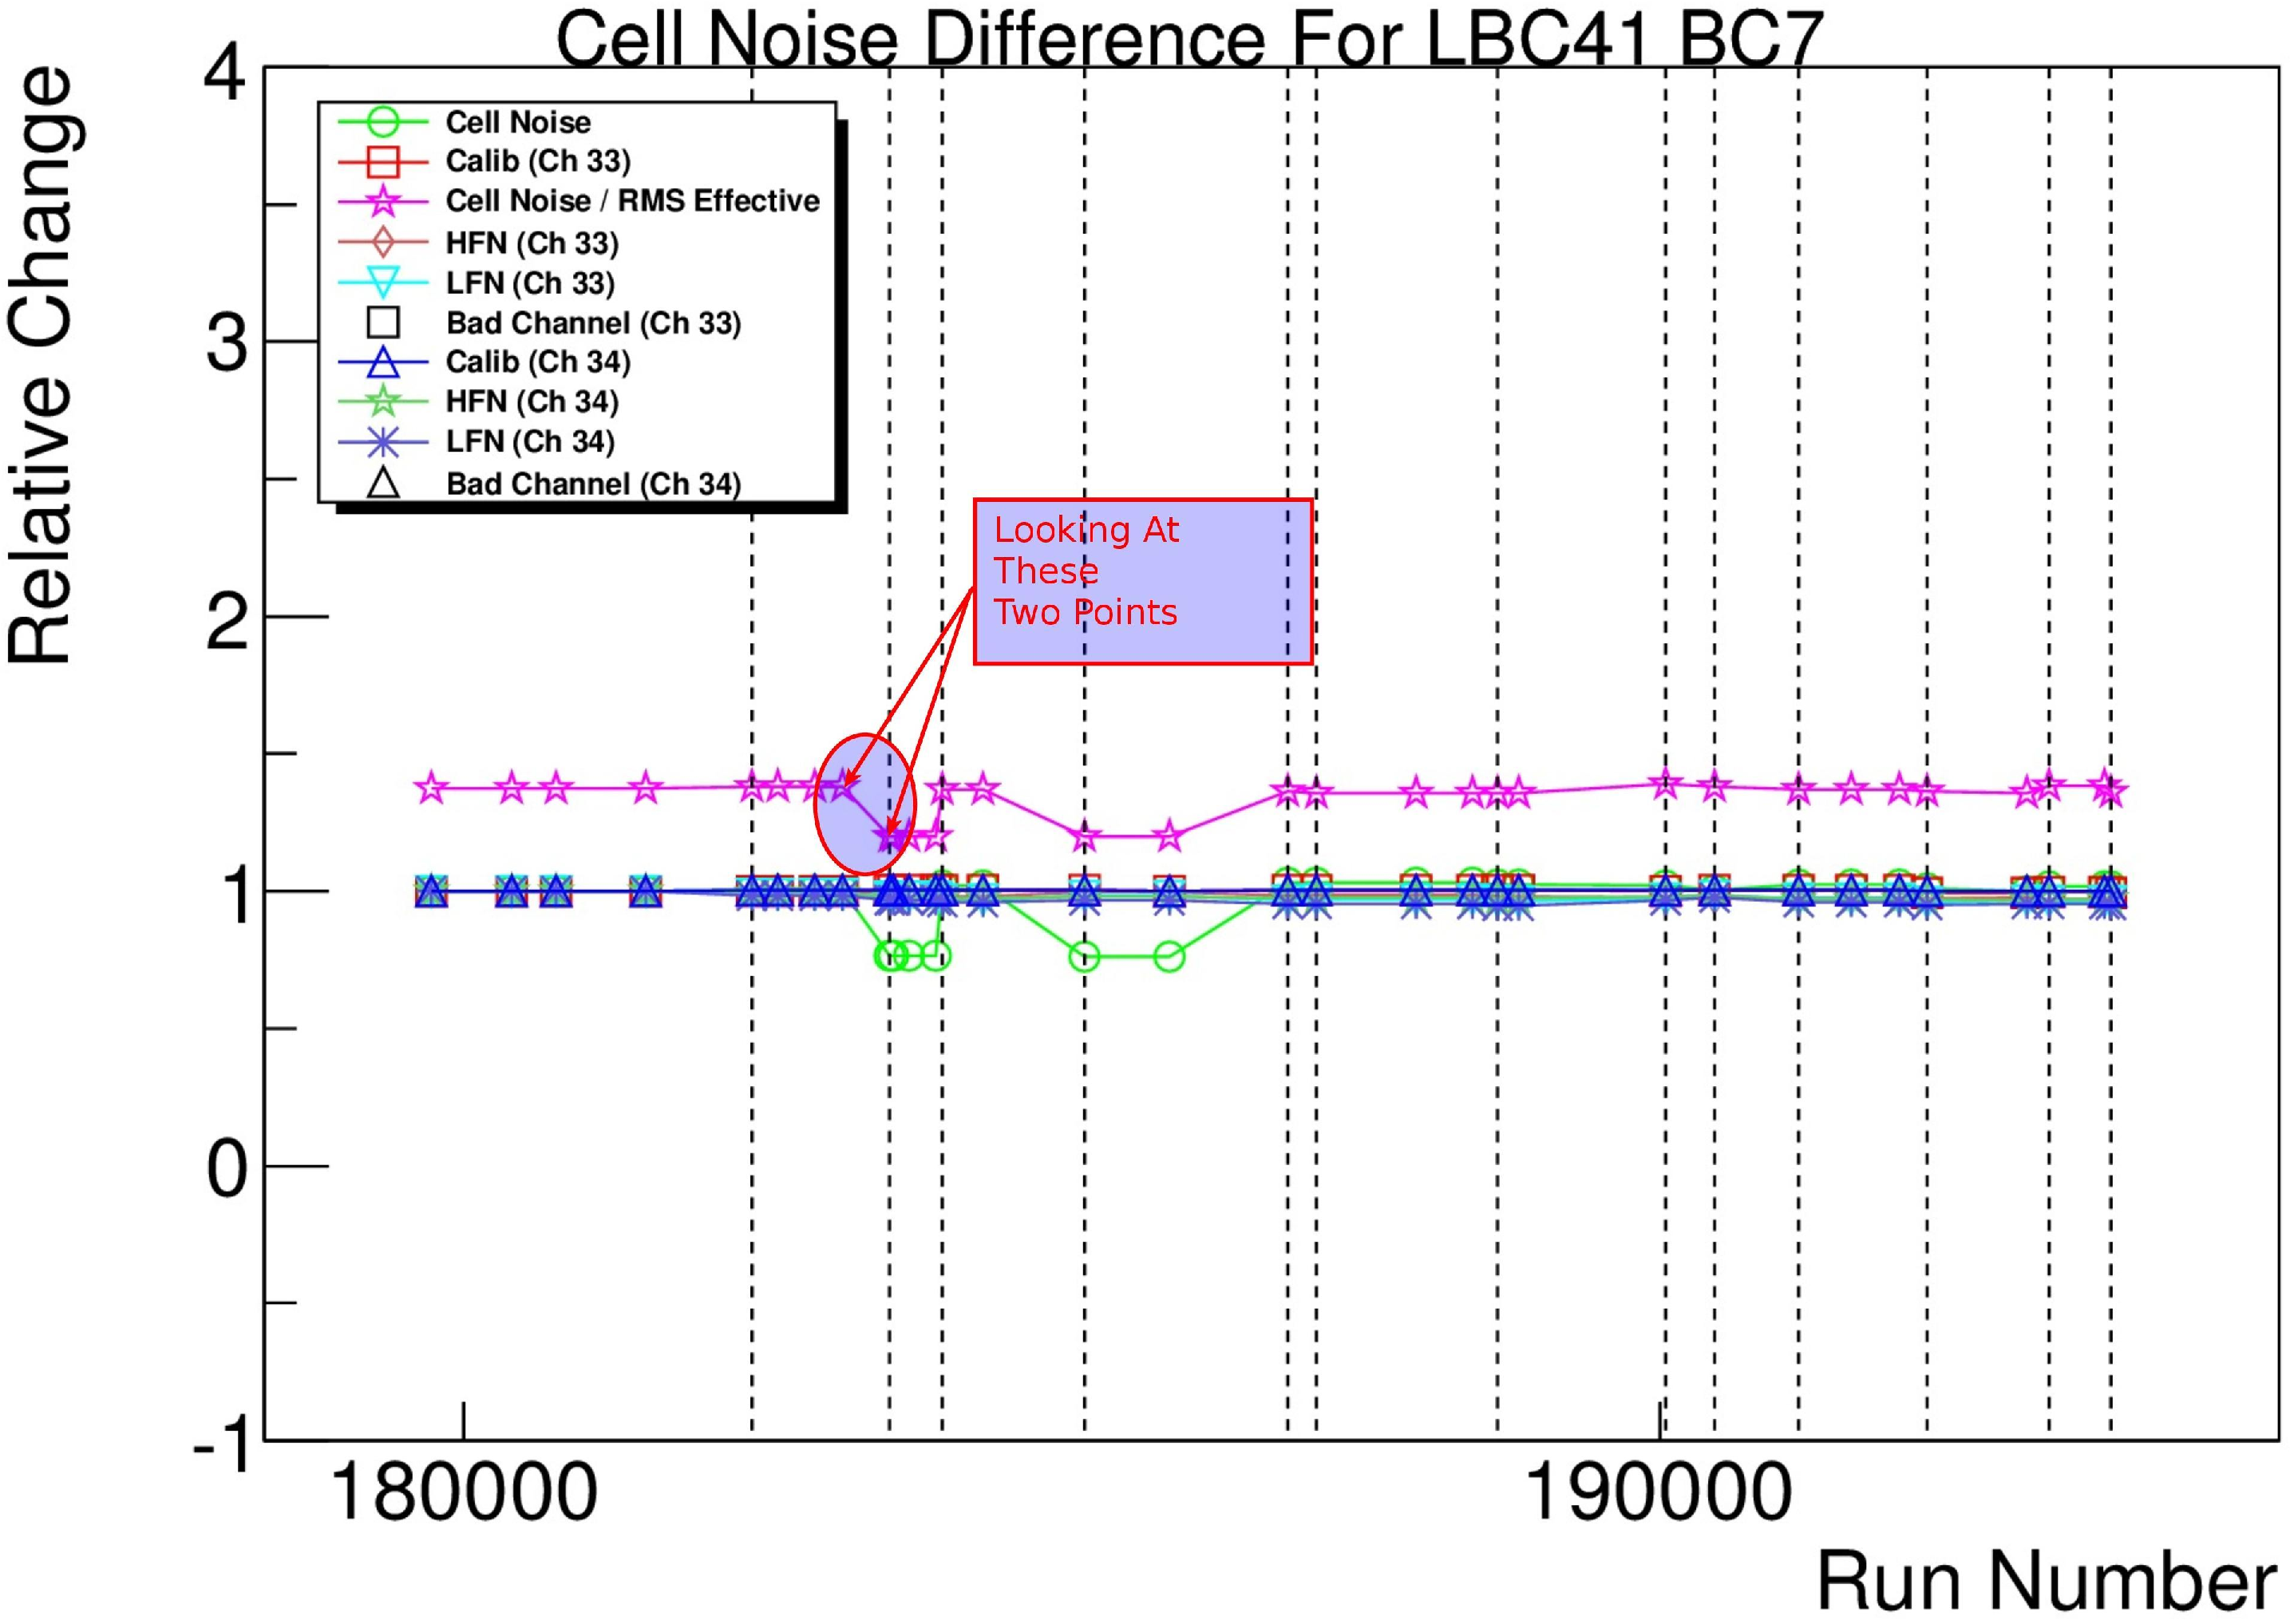
\includegraphics[width=\linewidth]{with_jumps}
    \caption{Cell with a variation.}
    \label{fig:with_jumps}
  \end{subfigure}
  \caption{Time evolution for two different representative cells in the
    calorimeter over the entire reprocessing period. The plot shows the change
    relative to the first run considered for several quantities for different
    IOVs (vertical dashed lines). If a channel is off due to some problems (Bad
    channel), this is reported in the plot with a black square.}
  \label{fig:jumps}
\end{figure}

This problem was investigated by re-performing the pedestal noise
fit\footnote{The standard calibration relies on automated fits performed by the
  ATLAS reconstruction. It was suspected at first that some of these fits were
  failing} manually and recalculating the noise constants focusing on two
specific IOVs, $[183110, 183382[$ (before the jump) and $[183382, 183515[$
(after the jump). Some calorimeter cells without jump were used to validate the
noise constants calculated with the fit and checked against the values stored in
COOL from automated fits performed by the standard ATLAS software.

\cref{fig:no_jump_fit} shows the control cell energy distribution with the
double Gaussian fit superimposed for two runs where the jump was present in
other cells. The results of the fit and the values stored in the COOL database,
both reported in \cref{tab:no_jump_fit}, are in good agreement.
\begin{table}[!h]
  \centering
  \begin{tabular}{r c c}
    \toprule
    \multicolumn{3}{c}{LBC41 BC2 Values Before Jump} \\
    \midrule \midrule
    \quad & Database  & Fit \\
    \midrule
    $\sigma_1$: & 19.97  & $20.08 \pm 0.05$ \\
    $\sigma_2$: & 80.59 & $77.3 \pm 9$ \\
    R\@: & 0.00026  & $0.0003 \pm 0.0012$\\
    \bottomrule
  \end{tabular} \quad
  \begin{tabular}{r c c}
    \toprule
    \multicolumn{3}{c}{LBC41 BC2 Values After Jump} \\
    \midrule \midrule
    \quad & Database & Fit \\
    \midrule
    $\sigma_1$: & 19.94 & $20.05 \pm 0.05$ \\
    $\sigma_2$: & 71.41 & $71.39 \pm 10.51$ \\
    R\@: & 0.00023 & $0.0002 \pm 0.0011$ \\
    \bottomrule
  \end{tabular}
  \caption{The table reports the comparison between the double Gaussian
    parameters stored in the COOL database and those obtained from the
    fit for two different run numbers corresponding to before and after the
    jump for a cell where there is no variation in the cell noise.}
\label{tab:no_jump_fit}
\end{table}

\begin{figure}[!h]
  \centering
  \begin{subfigure}[t]{.8\linewidth}
    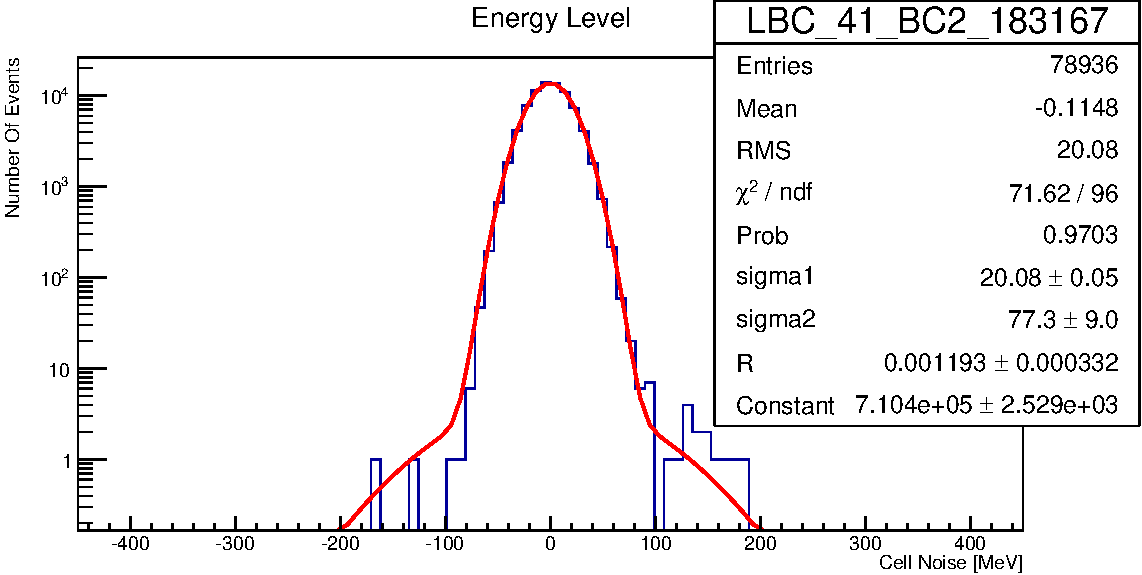
\includegraphics[width=\linewidth]{no_jump_fit_before}
    \caption{Fit before jump.}
    \label{fig:no_jump_fit_before}
  \end{subfigure}
  \begin{subfigure}[t]{.8\linewidth}
    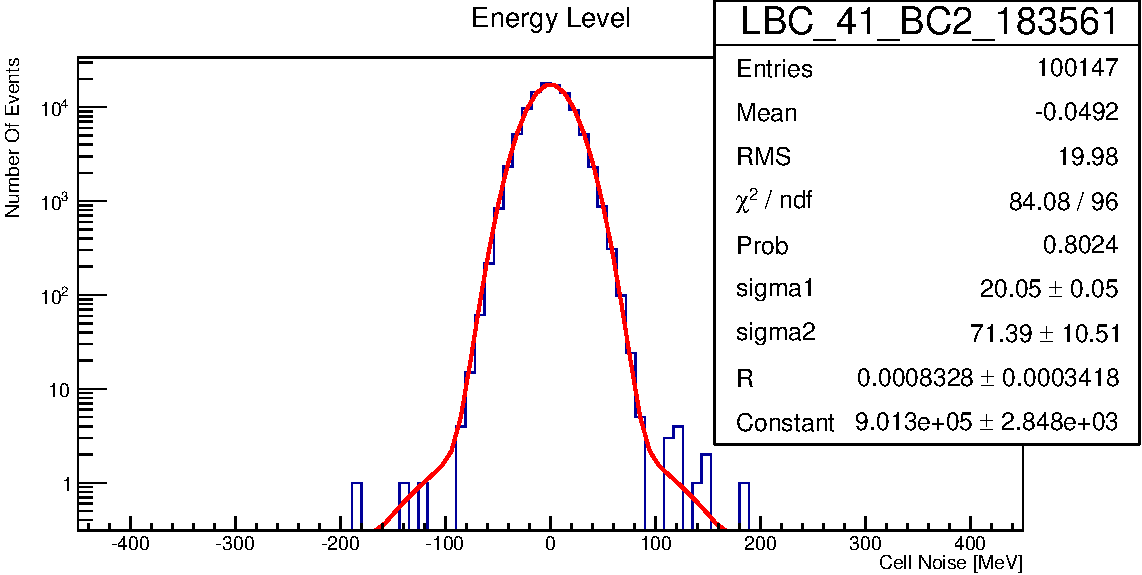
\includegraphics[width=\linewidth]{no_jump_fit_after}
    \caption{Fit after jump.}
    \label{fig:no_jump_fit_after}
  \end{subfigure}
  \caption{Fit of the reconstructed pulse shape on a control cell with no
    variation (jump) in the cell noise.}
  \label{fig:no_jump_fit}
\end{figure}

Moving to the investigation of a cell which exhibits the jump in the time
evolution the seventh cell of the BC layer (BC7) on the C side of the LB
partition of the 41st module (LBC 41) was selected for illustration purposes.
Figure~\ref{fig:jump_fit} shows the energy distribution with the double Gaussian
fit superimposed. The cell had the jump under investigation (see
Figure~\ref{fig:jumps}) and this is reflected in the fit results reported in
\cref{tab:jump_fit} together with the values from the database.
\begin{table}[!h]
  \centering
  \begin{tabular}{r c c}
    \toprule
    \multicolumn{3}{c}{LBC41 BC7 Values Before Jump} \\
    \midrule \midrule
    \quad & Database  & Fit \\
    \midrule
    $\sigma_1$: & 24.25  & $23.56 \pm 0.1$ \\
    $\sigma_2$: & 99.16 & $98.36 \pm 0.9$ \\
    R\@: & 0.037  & $0.042 \pm 0.036$ \\
    \bottomrule
  \end{tabular} \quad
  \begin{tabular}{r c c}
    \toprule
    \multicolumn{3}{c}{LBC41 BC7 Values After Jump} \\
    \midrule \midrule
    \quad & Database & Fit \\
    \midrule
    $\sigma_1$: & 24.42 & $24.4 \pm 0.1$ \\
    $\sigma_2$: & 94.56 & $94.55 \pm 1.34$ \\
    R\@: & 0.014 & $0.014 \pm 0.015$ \\
    \bottomrule
  \end{tabular}
  \caption{The table reports the comparison between the double Gaussian
    parameters stored in the COOL database and those obtained from the
    fit for two different run numbers corresponding to before and after the
    jump for a cell where a variation in the cell noise was spotted.}
  \label{tab:jump_fit}
\end{table}

Also in this case, the noise constants from the fit, are in agreement with those
stored in the COOL database. From this study it was concluded that bad fits
inside the automated ATLAS pedestal and noise reconstruction were not the cause
of the jumps. However, the $\chi^2$ of the distribution imply that the double
Gaussian model is not a good model for the second type of cells.
\begin{figure}[!h]
  \centering
  \begin{subfigure}[t]{.8\linewidth}
    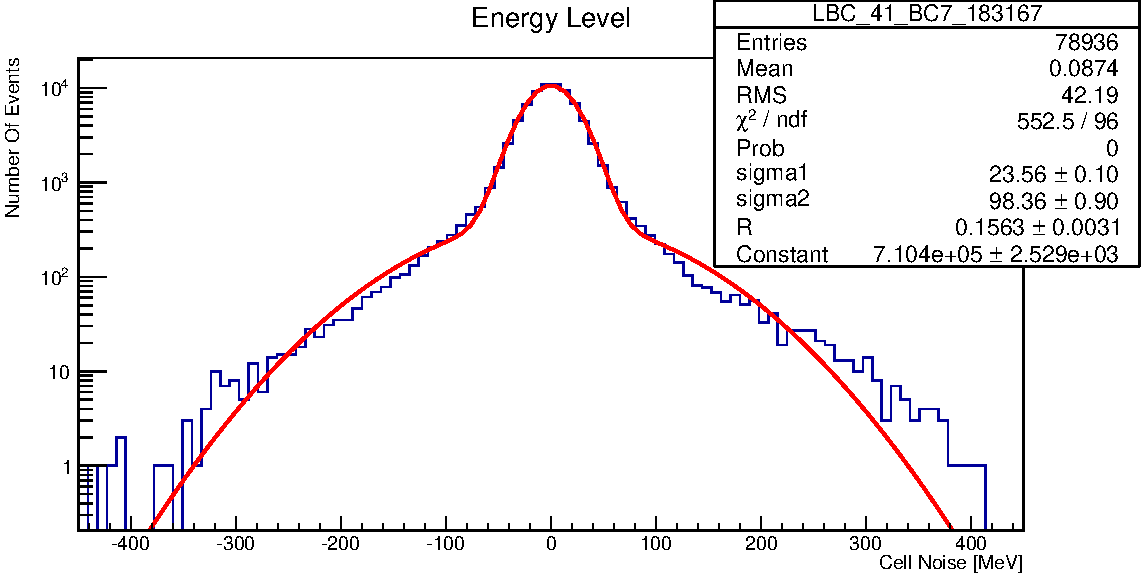
\includegraphics[width=\linewidth]{jump_fit_before}
    \caption{Before jump.}
    \label{fig:jump_fit_before}
  \end{subfigure}

  \begin{subfigure}[t]{.8\linewidth}
    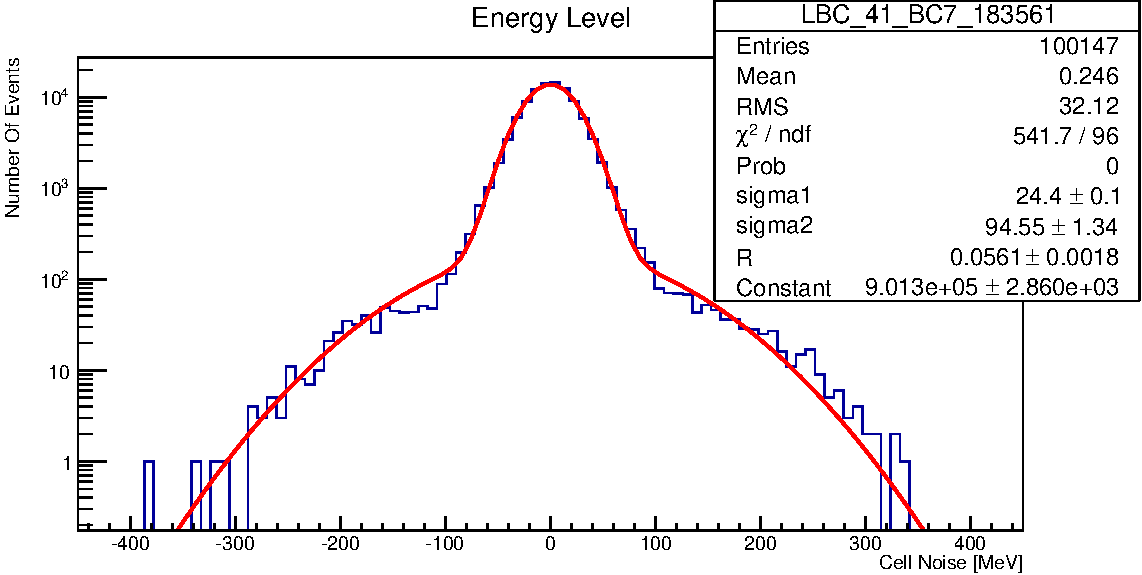
\includegraphics[width=\linewidth]{jump_fit_after}
    \caption{After jump.}
    \label{fig:jump_fit_after}
  \end{subfigure}
  \caption{Fit of the reconstructed pulse shape on a cell with variation (jump)
    in the cell noise non compatible with a change in the calibration, digital
    noise or channel status.}
  \label{fig:jump_fit}
\end{figure}

After further investigations it was discovered that this behavior is caused by
the \gls{tnf}. The electronic noise in nearby channels can be correlated. The
version of low voltage power supplies that were used during the 2011 data taking
lead to significant coherent noise among several channels, particularly those
close to the power supply (see \cref{fig:non_gaussianity}). Coherent noise means
that the signal in several cells can vary coherently and can thus alter the jet
and missing transverse energy reconstruction. In order to remedy this a Tile
Noise Filter was employed. The TNF calculates for each motherboard the pedestal
average:
\begin{equation}
  \label{eq:88}
  d = \frac{\sum_i^N d_i}{N}
\end{equation}
where the index $i$ runs over all the channels belonging to a certain
motherboard, $d_i$ is the $i$-th channel amplitude in ADC counts and $N$ is the
number of channels. Variations in this average baseline can be regarded as an
estimation of the coherent noise and is subtracted from the channel data of each
channel ($d_i - d$) on an event-by-event basis. In order to be able to perform
this noise filter calculation only channels without signal from physics are
taken into account in the sum of \cref{eq:88}.

The cell noise was recalculated without noise filter and the corresponding
distribution re-fitted. \cref{fig:no_filter_fit} show the double Gaussian fit
applied to another cell where the jump was present, in
\cref{fig:d2_fit_before,fig:d2_fit_after} the noise filter is on while in
\cref{fig:d2_fit_before_no_flt,fig:d2_fit_after_no_flt} the TNF was removed. It
can be seen that the fit improves when there is no noise filter. This shows that
the noise jump arises from bad fits when the TNF is somehow malfunctioning and
transforms a double Gaussian distribution into a distribution with more
complicated shape.
\begin{figure}[!h]
  \centering
  \begin{subfigure}[t]{.48\linewidth}
    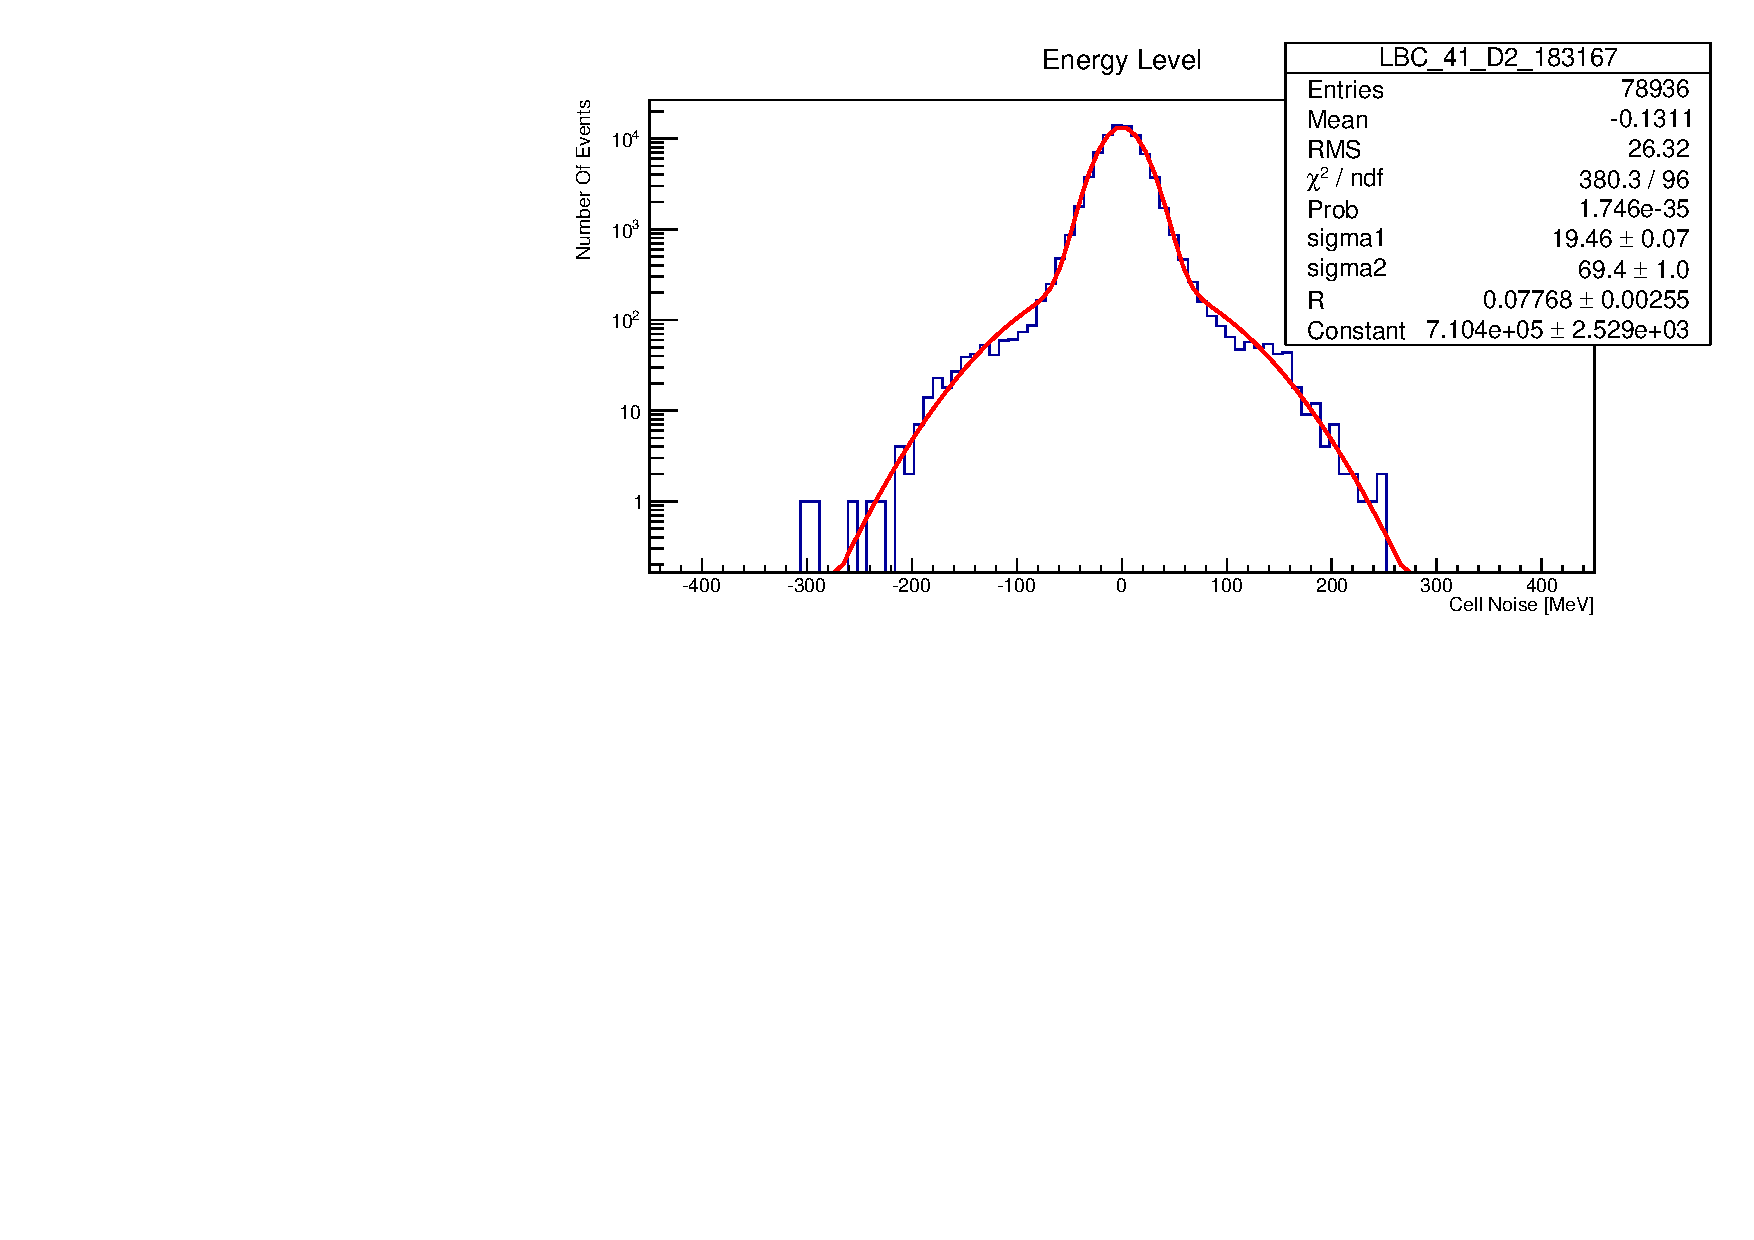
\includegraphics[width=\linewidth]{d2_fit_before}
    \caption{Before jump.}
    \label{fig:d2_fit_before}
  \end{subfigure}
  \begin{subfigure}[t]{.48\linewidth}
    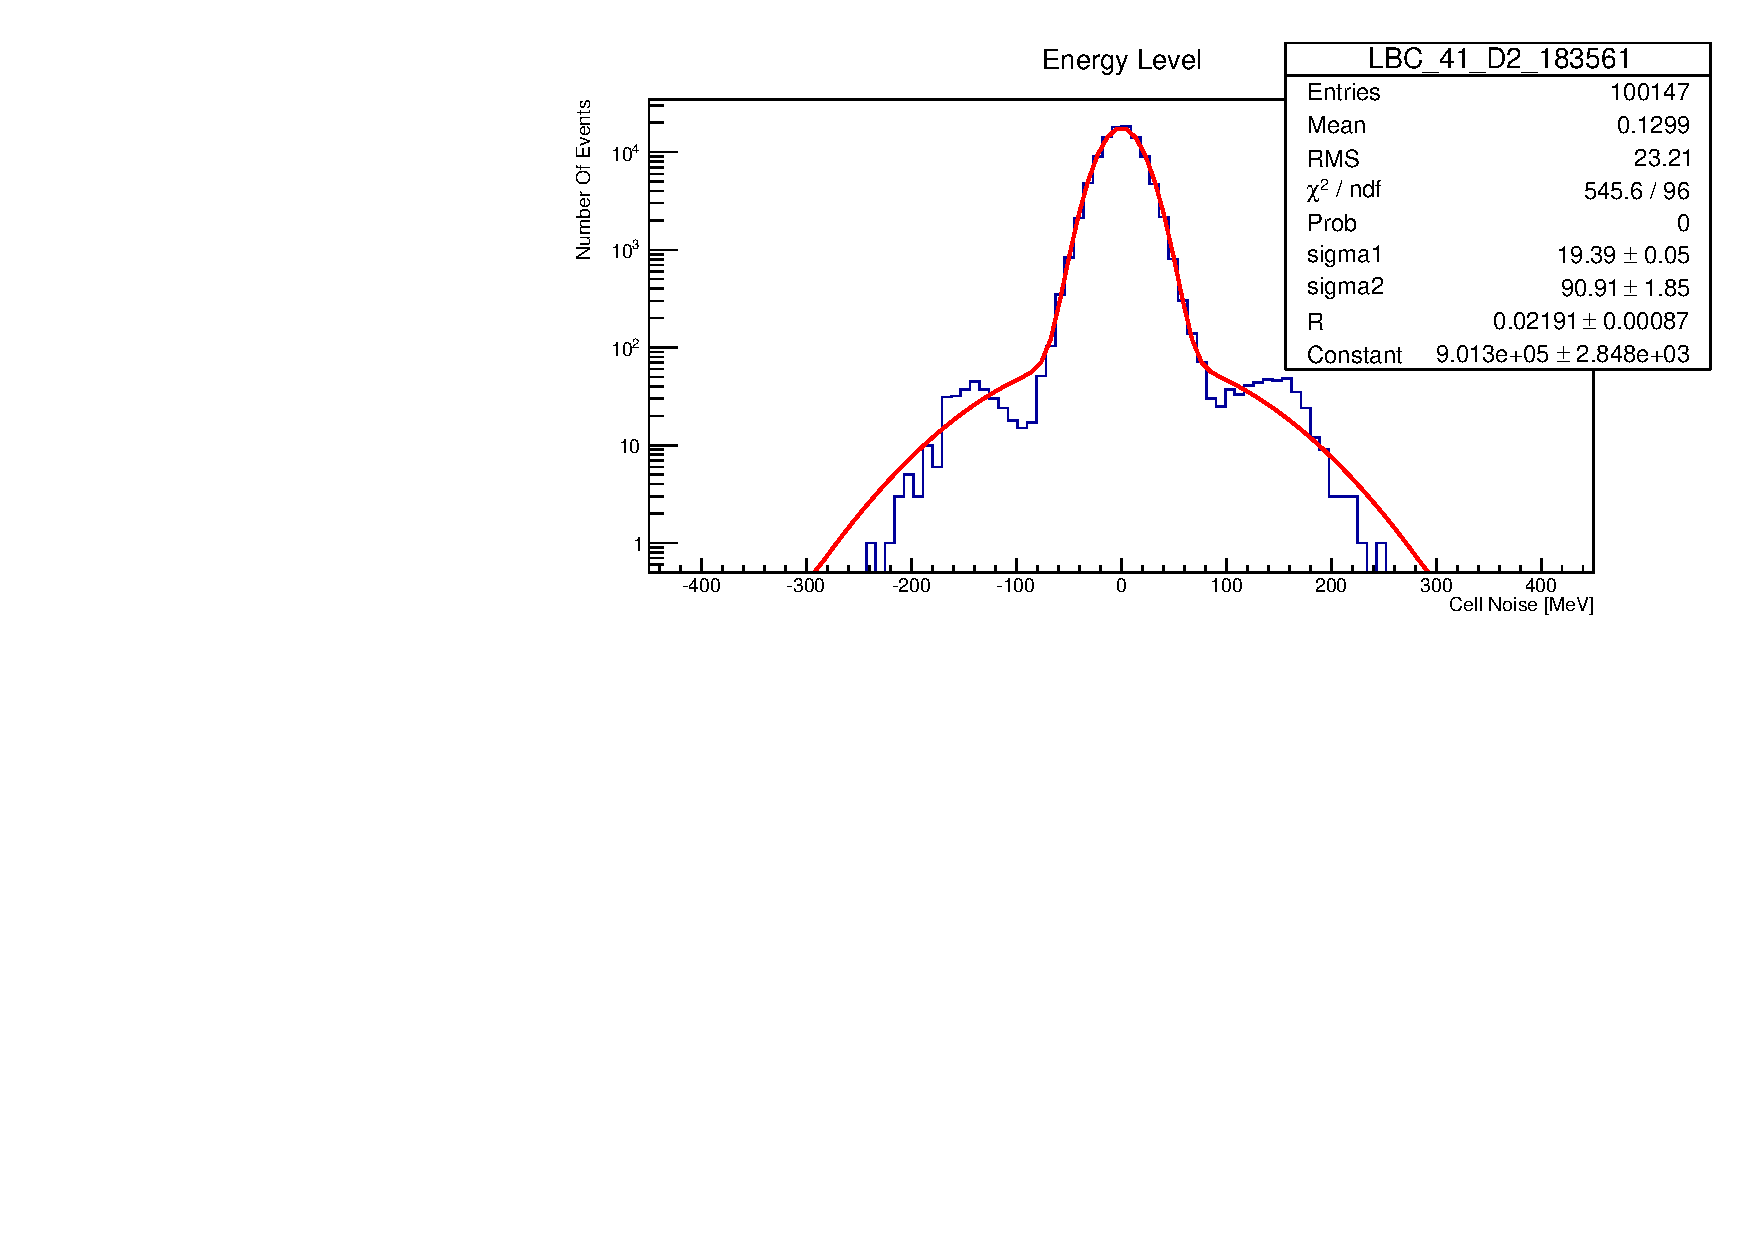
\includegraphics[width=\linewidth]{d2_fit_after}
    \caption{After jump.}
    \label{fig:d2_fit_after}
  \end{subfigure}

  \begin{subfigure}[t]{.48\linewidth}
    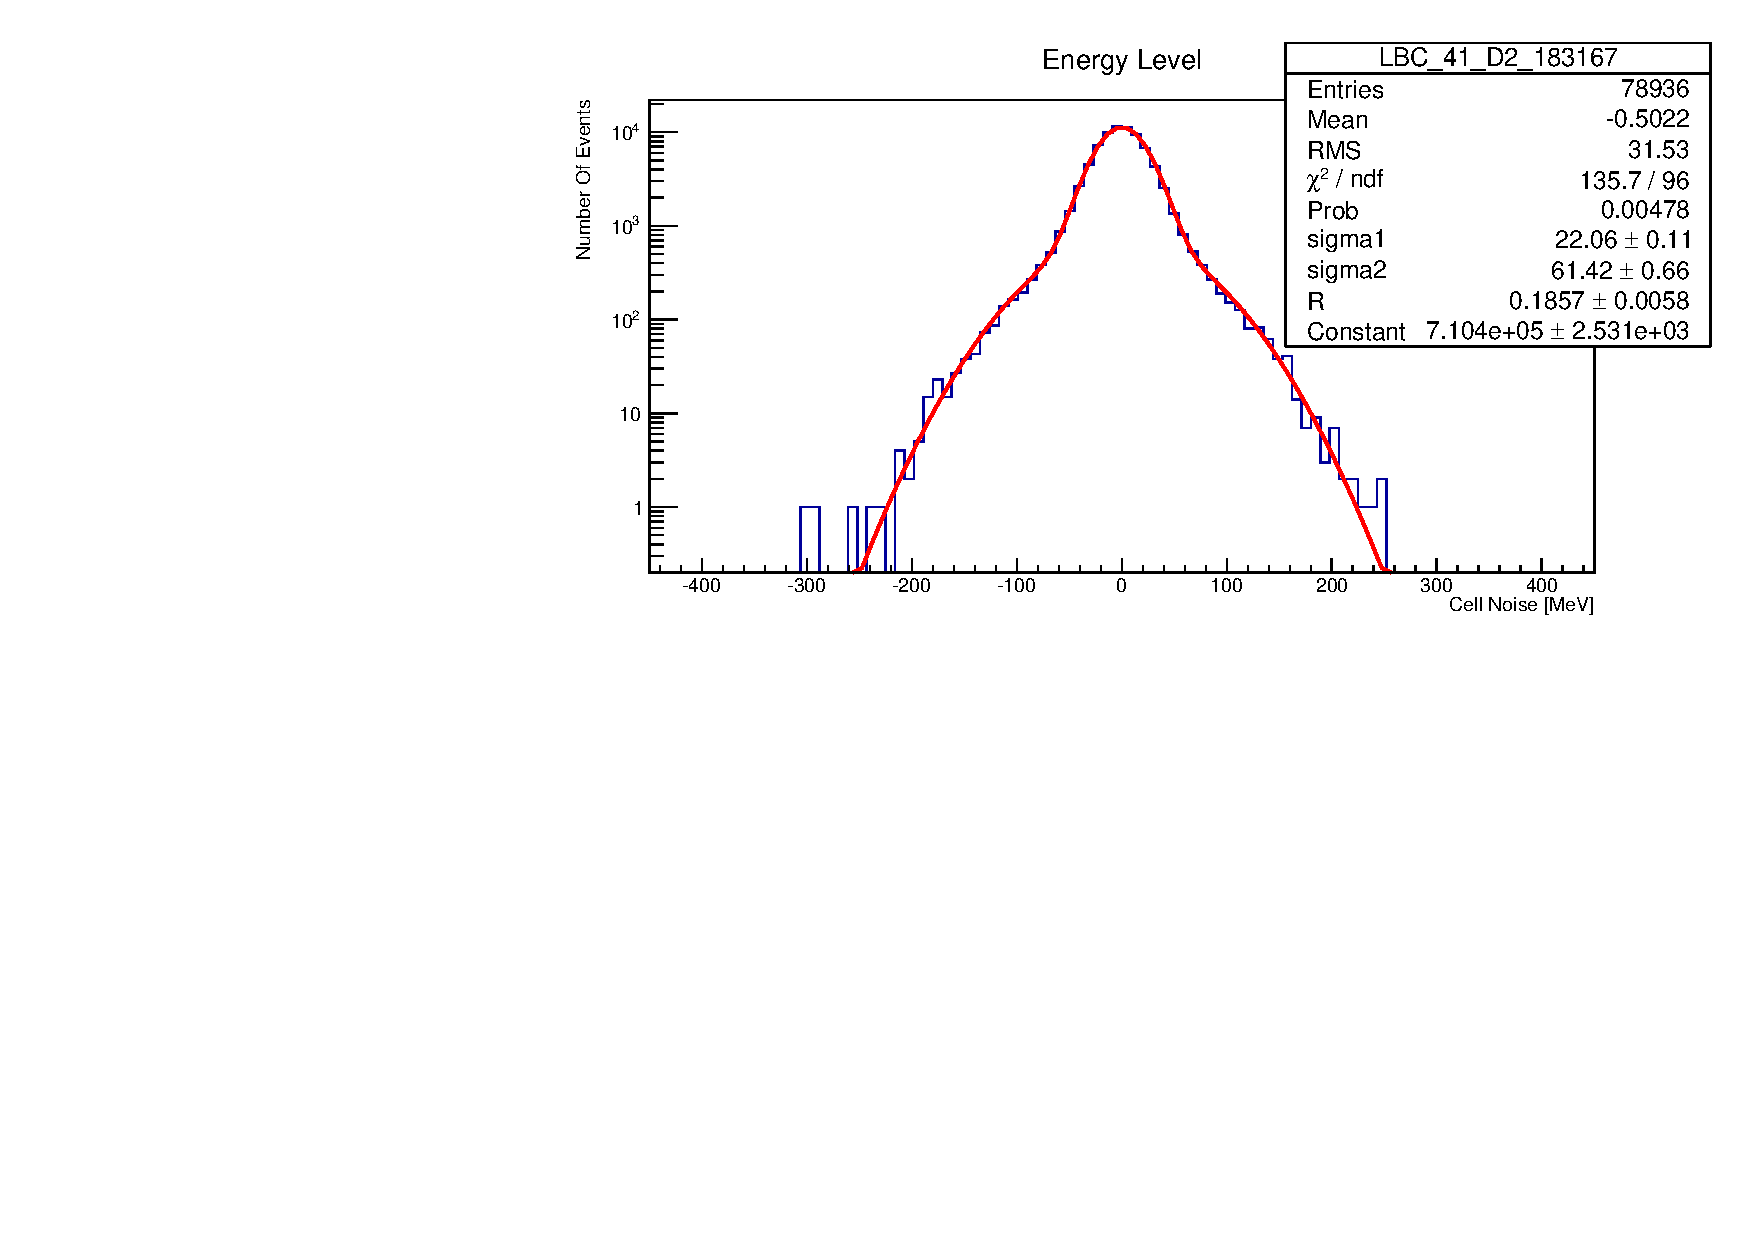
\includegraphics[width=\linewidth]{d2_fit_before_no_flt}
    \caption{Before jump.}
    \label{fig:d2_fit_before_no_flt}
  \end{subfigure}
  \begin{subfigure}[t]{.48\linewidth}
    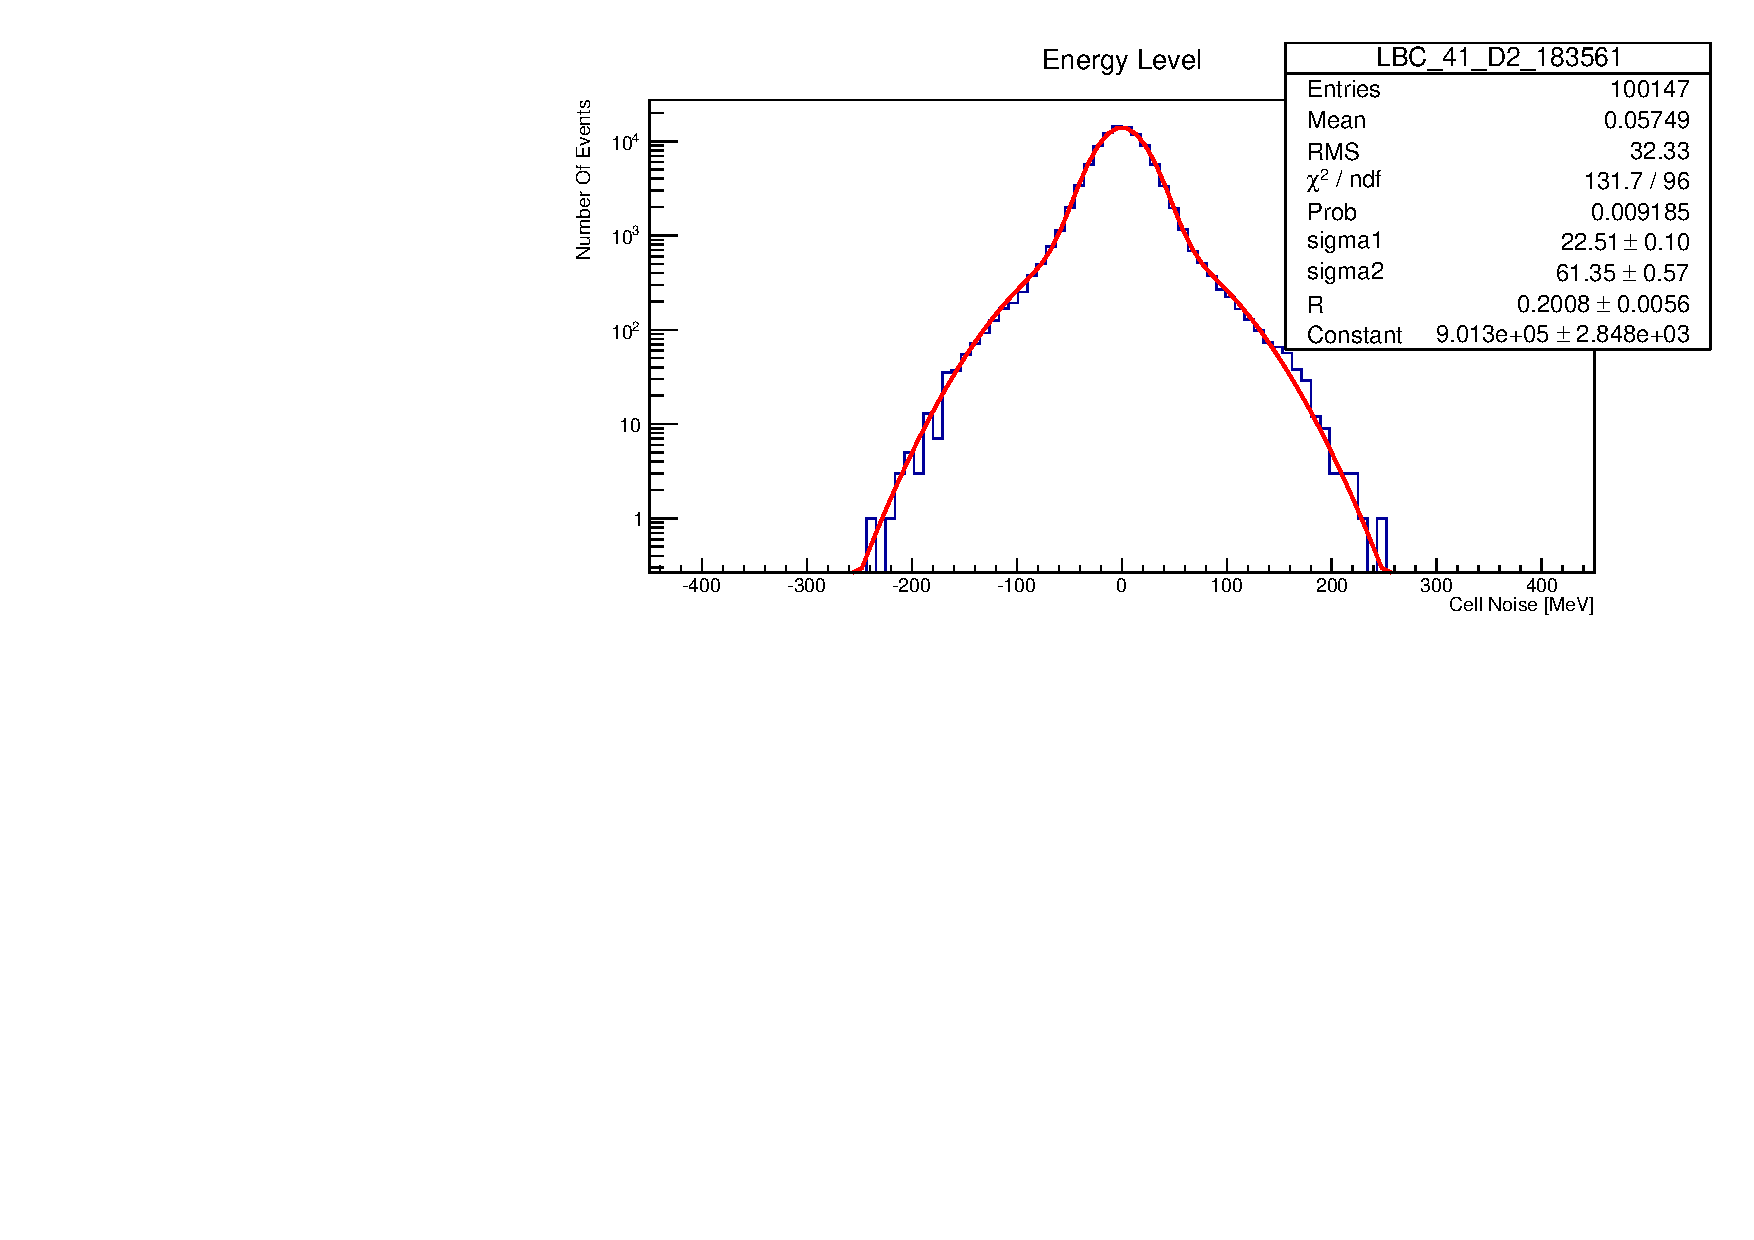
\includegraphics[width=\linewidth]{d2_fit_after_no_flt}
    \caption{After jump.}
    \label{fig:d2_fit_after_no_flt}
  \end{subfigure}
  \caption{Comparison of the reconstructed pulse shape of a cell with the cell
    noise variation without a corresponding variation in he calibration
    constants, digital noise or channel status (jump) with the double Gaussian
    fit superimposed with the noise filter
    (\cref{fig:d2_fit_before,fig:d2_fit_after}) and without noise filter
    (\cref{fig:d2_fit_before_no_flt,fig:d2_fit_after_no_flt}).}
  \label{fig:no_filter_fit}
\end{figure}
%%% Local Variables:
%%% mode: latex
%%% TeX-master: "../search_for_DM_LED_with_ATLAS"
%%% End:


\section{Conclusions}
\label{sec:conclusions}

In 2013 the ATLAS 2011 data was reprocessed with improved algorithms and
calibrations. In TileCal the methods to produce Cs and laser calibration
constants were improved and required a re-computation of the TileCal noise
constants. Changing the calibration constants, according to \cref{eq:70},
changes the reconstructed energy in the cell thus affecting the jet
identification (see \cref{sec:topocluster}). A comparison between the
$\phi$--averaged RMS of electronic cell noise as a function of $\eta$ of the
cell before and after reprocessing for the high statistic run 192130 with both
channels in high gain is shown in \cref{fig:noise_avg_old_new_hghg}. There is a
general increase of the cell noise of about 0.5\% in the EBC, LBC and EBA
partitions. The LBA partition had module 22 running in \emph{emergency mode},
i.e.\ operated with $\sim$ 50~V less high voltage on the PMTs, and had the
cesium calibration constants updated. This change is likely to have lowered the
average noise in this partition.

\begin{figure}[!h]
  \centering
    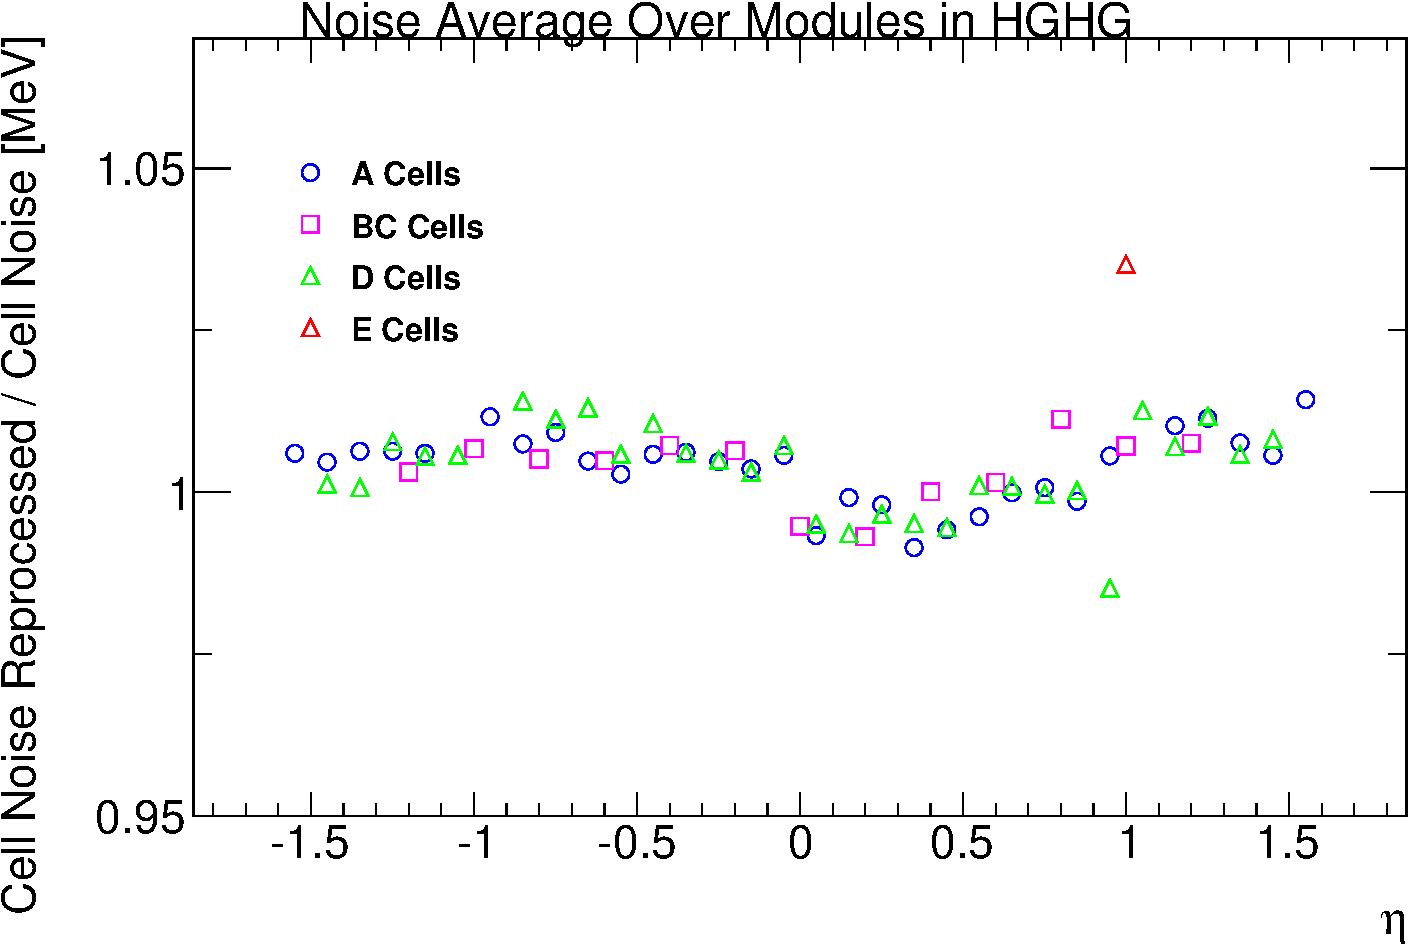
\includegraphics[width=.8\linewidth]{noise_avg_old_new_192130_hghg}
    \caption{Comparison between the $\phi$--averaged RMS of electronic cell
      noise as a function of $\eta$ of the cell before and after reprocessing
      for the high statistic 192130 run with both channels in high gain. The
      different layers are shown separately, A, BC, D and E (gap/crack). The
      transition between the long and extended barrels can be seen in the range
      $0.7 < |\eta| < 1.0$.}
    \label{fig:noise_avg_old_new_hghg}
\end{figure}

The change of the cell noise between IOVs was monitored using a special software
within the TUCS environment. A problem with the TNF has been identified in cells
which exhibits a variation in the cell noise without a corresponding variation
in other relevant quantities were present. The number of cells affected by this
problem is investigated constructing the distribution of the ratio $\sigma$ /
RMS$_\mathrm{\, eff}$ shown in \cref{fig:all_rms_eff}. The bulk of the
distribution have $\sigma$~/~RMS$_\mathrm{\, eff}$ close to one, this
corresponds to cells for which the double Gaussian noise is a good model. There
is nevertheless a big tail of cells with $\sigma$~/~RMS$_\mathrm{\, eff}$ up to
1.7, with about 5\% of the cells with $\sigma$~/~RMS$_\mathrm{\, eff}$ larger
than 1.2. After the installation of the new LVPS the contribution from a second
wider Gaussian to the electronic noise is much smaller and the effect of the TNF
is expected to be smaller as well. However the effect of the TNF with the new
power supplies remains to be checked.
\begin{figure}[!h]
  \centering
    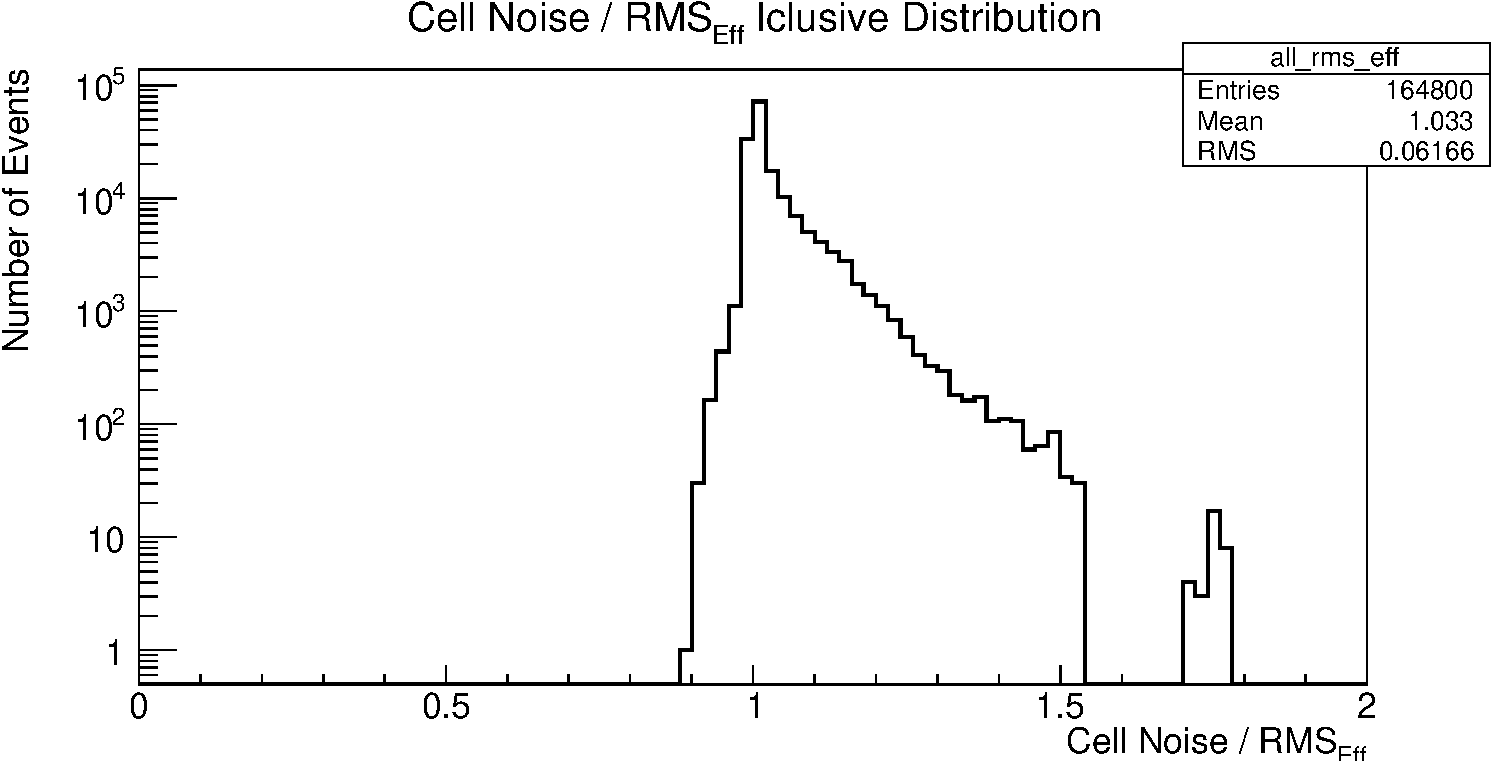
\includegraphics[width=.8\linewidth]{all_rms_eff}
    \caption{Distribution of the ratio $\sigma$ / RMS$_\mathrm{\, eff}$ where the
      $\sigma$ and RMS$_\mathrm{\, eff}$ values are taken from all IOVs
      considered for the 2011 TileCal reprocessing.}
    \label{fig:all_rms_eff}
\end{figure}
%%% Local Variables:
%%% mode: latex
%%% TeX-master: "../search_for_DM_LED_with_ATLAS"
%%% End:


\chapter{Physical Objects Reconstruction}
\label{cha:phys-objects-reconst}

Object reconstruction is the process that associates the signal left in the
detector by charged particles to physical objects through a series of
algorithms. This analysis uses electrons, muons, jets and missing transverse
momentum ($\met$). Two types of electrons, muons and jets are also defined:
\emph{baseline} and \emph{good}, where the former one is used for removal of
overlapping objects and preselection while the latter for selecting the objects
used to define the signal and control regions. In the following a brief
introduction to the identification criteria of these objects is presented.
%%% Local Variables:
%%% mode: latex
%%% TeX-master: "../search_for_DM_LED_with_ATLAS"
%%% End:


\section{Primary Vertex}
\label{sec:primary-vertex}

In $pp$ collisions with high luminosity, multiple interactions occur on a given
bunch crossing, the spatial location of the a $pp$ collision is called \gls{pv},
the one that has the highest $\sum \pt^2$ of constituent tracks is known as
\gls{hs} vertex, the rest are called \emph{pile-up vertices}. The
reconstruction of the PV generally happens in two stages that are often not
distinguishable from each other. The \emph{vertex finding} associates
reconstructed tracks to a particular vertex candidate and the \emph{vertex
  fitting} reconstructs the actual vertex position, refits the tracks and
estimates the quality of the fit~\cite{PV}.

In the current analysis, events are required to have at least one PV with two
associated tracks.
%%% Local Variables:
%%% mode: latex
%%% TeX-master: "../search_for_DM_LED_with_ATLAS"
%%% End:


\section{Track reconstruction}
\label{sec:track-reconstruction}

Charged particles that move through the solenoidal magnetic field that surrounds
the ATLAS tracking system, follow helical trajectories. The projection of a
helix on the $xy$ plane is a circle and, in order to uniquely parametrize the
particle track in three dimensions, five parameters are needed. A common choice
is to use the \emph{perigee} parameters, where the perigee is the point of
closest approach to the beam axis. With this choice, the five parameters are:
\begin{itemize}
\item The signed curvature $C$ of the helix, defined as $C = q / 2R$ where $q$
  is the particle charge and $R$ is the radius of the helix. This is related to
  the transverse momentum $\pt = qB / C$, where $B$ is the magnetic field
  measured in Tesla, C is measured in m$^{-1}$ and $\pt$ in GeV.
\item The distance of closest approach $d_0$ in the $xy$ plane measured in
  millimeters.
\item The $z$ coordinate of the point of closest approach, denoted by $z_0$ and
  measured in millimeters.
\item The azimuthal angle $\phi_0$ of the tangent to this point.
\item The polar angle $\theta$ to the $z$-axis.
\end{itemize}
The perigee and the track parameters are schematized in
Figure~\ref{fig:track_par}.
\begin{figure}[!h]
  \centering
    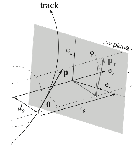
\includegraphics[width=.8\linewidth]{track_parameters}
    \caption{Track parameters at the perigee. In the figure \textbf{p} is the
      momentum of the incoming particle, e$_\mathrm{x}$, e$_\mathrm{y}$,
      e$_\mathrm{z}$ are the coordinate system defined in
      \cref{sec:coordinate-system} and $\theta$ and $\phi$, also defined in
      \cref{sec:coordinate-system} are the polar and azimuthal angle
      respectively.}
    \label{fig:track_par}
\end{figure}
%%% Local Variables:
%%% mode: latex
%%% TeX-master: "../search_for_DM_LED_with_ATLAS"
%%% End:


\section{Electrons}
\label{sec:electrons}

Electrons are identified in the central part of the ATLAS detector
($|\eta| < 2.47$) by an energy deposit in the electromagnetic calorimeter and an
associated track in the inner detector. Signal electrons are defined as prompt
electrons coming from the decay of a $W, Z$ boson or a top quark while
background non-prompt electrons come from hadron decays, photon conversion,
semi-leptonic heavy flavor hadron decay and highly electromagnetic jets. To
differentiate between signal and background electrons a likelihood discriminant
is formed using different information: the shower shape in the EM calorimeter,
the track-cluster matching, some of the track quality distributions from signal
and background simulation and cuts on the number of hits in the ID\@. Cuts that
depend on $|\eta|$ and $\et$ on the likelihood estimator allow to distinguish
between signal and background electrons. To further enhance the discrimination
from background electrons signal electrons are required to be separated from
other detector activity, this is done by requiring the energy deposited by the
electron in the calorimeter or the scalar sum of the transverse momentum of the
tracks in the \gls{id} contained in a cone of some specified size $\Delta R$ to
be less than a threshold value that depends on the tightness of the electron
identification required. These track or calorimeter based criteria are commonly
referred to as \emph{isolation}.

Electron identification efficiencies are measured in $pp$ collision data and
compared to efficiencies measured in $\zee$ simulations. Signal electrons can
furthermore be selected with different sets of cuts for the likelihood-based
criteria with $\sim 95\%, \sim 90\%$ and $\sim 80\%$ efficiency for electrons
with $\pt = 40~$GeV. The different criteria are referred to as \emph{loose},
\emph{medium} and \emph{tight} operating points respectively~\cite{ATL-EL-IDENT}
where, for example, the tight criterion leads to a higher purity of signal
electrons but has a lower efficiency than the looser criteria.

In this analysis, the \emph{baseline electrons} are selected requiring a
transverse energy $\et > 20$~GeV, $|\eta| < 2.47$, they need to satisfy the
\emph{loose} likelihood selection criteria, it is required that no dead EM
calorimeter \gls{feb} or \gls{hv} channels in the calorimeter cluster are
present and that the baseline electron survives the overlap removal with other
particles as described in \cref{sec:overlap-removal}. The baseline electron
criteria is used to veto electrons used in the muon control regions and the
signal region definition. In addition to all the baseline criteria, the
\emph{good electron} definition requires the electrons to satisfy the
\emph{tight} likelihood selection criteria, the electron track
$d_0 / \sigma_{d0} < 5$ and $|z_0| < 0.5$~mm and the \emph{LooseTrackOnly}
electron isolation criteria which is based only on tracks and is set to be 99\%
efficient. \cref{tab:ele_def} summarizes the selection criteria for the
electrons in the monojet analysis.
\begin{table}[!th]
  \centering
  \begin{tabular}{ll}
    \toprule
    \multicolumn{2}{c}{Electron Definition} \\
    \midrule \midrule
    \textbf{Baseline electron} & \textbf{Good electron} \\
    \midrule
    $\et > 20$~GeV & \emph{baseline} \\
    $|\eta| < 2.47$ & \emph{tight} working point \\
    \emph{loose} working point & $d_0 / \sigma_{d0} < 5$ \\
    No dead FEB in the EM calo cluster & $|z_0| < 0.5$~mm \\
    No dead HV in the EM calo cluster & \emph{LooseTrackOnly} \\
    passes the overlap removal & \\
    \bottomrule
  \end{tabular}
  \caption{Electron definition for the monojet analysis.}
  \label{tab:ele_def}
\end{table}
%%% Local Variables:
%%% mode: latex
%%% TeX-master: "../search_for_DM_LED_with_ATLAS"
%%% End:


\section{Muons}
\label{sec:muons}

Muons are identified using different criteria from the information provided by
the ID and the MS leading to four different types of muons. The \gls{sa} muons
use only the MS information to reconstruct the muon's trajectory; the \gls{cb},
where the track is independently reconstructed in the ID and the MS and then
combined; the \gls{st} are identified as muons only if the track in the ID is,
after being extrapolated to the MS, associated to at least one local track
segment in the MDT or CSC chambers and finally the \gls{ct} where tracks in the
ID are associated to an energy deposit in the calorimeter compatible with a
minimum ionizing particle. CB candidates perform best in terms of muon purity
and momentum resolution.

Muons are identified using quality requirements specific to each of the four
type of muons aiming at rejecting those coming from pion and kaon decays and
guarantee a robust momentum measurement. The \emph{loose} identification
criteria maximize the reconstruction efficiency and provide good muon tracks;
the \emph{medium} criteria minimize the systematic uncertainties associated to
muon reconstruction and calibration; the \emph{tight} muons maximize the purity
of the sample and the \emph{high $\pt$} selection maximize the momentum
resolution for tracks with transverse momenta above 100~GeV~\cite{MUONS}.

This analysis uses the CB muons that pass the medium identification criteria,
moreover the \emph{baseline muons} are required to have $\pt > 10$~GeV and
$|\eta| < 2.5$, the $\met$ definition and in the lepton veto used to define the
signal and control regions. The \emph{good muons} are required to pass the
baseline selection criteria, moreover $d_0 / \sigma_{d0} < 3$,
$|z_0 \sin \theta| < 0.5$~mm. The good muons are used in the one muon and
di-muon control regions.

\begin{table}[!th]
  \centering
  \begin{tabular}{ll}
    \toprule
    \multicolumn{2}{c}{Muon Definition} \\
    \midrule \midrule
    \textbf{Baseline muon} & \textbf{Good muon} \\
    \midrule
    CB muon & \emph{baseline} \\
    \emph{Medium} id. criteria & $d_0 / \sigma_{d0} < 3$ \\
    $\pt > 10$~GeV & $|z_0 \sin \theta| < 0.5$~mm \\
    $|\eta| < 2.5$ & \\
    passes the overlap removal & \\
    \bottomrule
  \end{tabular}
  \caption{Muon definitions for the monojet analysis.}
  \label{tab:ele_def}
\end{table}
%%% Local Variables:
%%% mode: latex
%%% TeX-master: "../search_for_DM_LED_with_ATLAS"
%%% End:


\section{Topocluster}
\label{sec:topocluster}

The cell noise described in \cref{sec:cell-noise} is used in the
\emph{topological clustering} algorithm~\cite{JetCluster}, for identification of
the real energy deposits in the calorimeters. The algorithm assumes that the
noise in all the calorimeter cells is normally distributed with significance
(the ratio between the deposited energy and the parameter $\sigma$ used to
describe the cell noise) expressed in units of Gaussian sigmas. In the
algorithm, cluster of cells called \emph{topoclusters}, are formed by comparing
the energy deposit in a cell for a significant incompatibility with a noise only
hypothesis. The algorithm starts by finding the \emph{seed cells} with
$E > 4 \sigma$ where $\sigma$ is the measured RMS of the energy distribution for
every cell in the pedestal run. The second step is to add to the seeds neighbor
cells that satisfy the $E > 2 \sigma$ condition. Finally an additional level of
cells with $E > 0$ is added to the perimeter of the cluster and the algorithm is
ended. At this point the splitting algorithm is applied to separate the
topoclusters based on the local energy maxima.
%%% Local Variables:
%%% mode: latex
%%% TeX-master: "../search_for_DM_LED_with_ATLAS"
%%% End:


\section{Jets}
\label{sec:jets}

The quarks and gluons that carry color charge and are created in the scattering
process, hadronize producing collimated bunches of colorless hadrons (jets)
which keep track of the energy and direction of the originating parton. Jets in
ATLAS are reconstructed as massless particles using the \emph{$\antikt$}
algorithm, calibrated and corrected for pile--up contamination. These steps are
briefly outlined in the next sections.
%%% Local Variables:
%%% mode: latex
%%% TeX-master: "../search_for_DM_LED_with_ATLAS"
%%% End:


\subsection{The \emph{$\antikt$} Algorithm}
\label{sec:anti-k_t}

The $\antikt$ algorithm is a sequential recombination algorithm. It defines two
distances $d_{ij}$ and $d_{iB}$. The distance $d_{ij}$ between the physical
objects $i$ and $j$ is defined as:
\begin{equation}
  \label{eq:89}
  d_{ij} = \min(k_{ti}^{-2}, k_{tj}^{-2}) \frac{\Delta_{ij}^2}{R^2}
\end{equation}
where $\Delta_{ij}^2 = (\eta_i - \eta_j)^2 + (\phi_i^2 - \phi_j^2)$ and $\eta_i$
is the rapidity, $\phi_i$ is the azimuthal angle, $k_{ti}$ is the transverse
momentum of the object $i$ and $R$ is the radius parameter that controls the
size of the jet. The distance $d_{iB}$ between the object $i$ and the beam (B)
defined as:
\begin{equation}
  \label{eq:90}
  d_{iB} = k_{ti}^{-2}.
\end{equation}
This distance is meant to distinguish between hard and soft terms. The algorithm
identifies the smallest of the two distances and, if it is $d_{ij}$, it
recombines the $i$ and $j$ objects while if it is $d_{iB}$, it calls $i$ a jet
and removes it from the list of inputs to the algorithm. The distances are
recalculated and the procedure reiterated until there are no more
objects~\cite{Antikt}.
%%% Local Variables:
%%% mode: latex
%%% TeX-master: "../search_for_DM_LED_with_ATLAS"
%%% End:


\subsection{The Jet Vertex Tagger }
\label{sec:jet-vertex-tagger}

The excess transverse energy coming from pile-up jets is generally subtracted on
average from the signal energy, however, due to localized fluctuations in the
pile-up, some of it remains in the $\pt$ of the reconstructed jet. The \gls{jvf}
is a variable that uses information from the track associated to each jet to
identify the origin vertex of each jet and rejects it if not coming from a
hard-scatter vertex~\cite{JVF}. The JVF can be regarded as a measure of the
fraction of the jet momentum associated with a primary vertex and is defined as:
\begin{equation}
  \label{eq:91}
  \mathrm{JVF} = \frac{\sum_k p_\mathrm{\, T}^\mathrm{\, trk_k}
    (\mathrm{PV_0})}{\sum_l p_\mathrm{\, T}^\mathrm{\, trk_l} (\mathrm{PV_0}) +
    \sum_{n \geq l} \sum_k p_\mathrm{\, T}^\mathrm{\, trk_l} (\mathrm{PV_n})}
\end{equation}
where PV$_0$ is the hard scatter vertex and PV$_\mathrm{n}$ with
$\mathrm{n} \geq 1$ is any other pile--up PV in the same bunch crossing thus
$\sum_k p_\mathrm{\, T}^\mathrm{\, trk_k} (\mathrm{PV_0})$ is the scalar $\pt$
sum of the tracks associated with the jet and originating from the hard scatter
vertex while
$\sum_{n \geq l} \sum_k p_\mathrm{\, T}^\mathrm{\, trk_l} (\mathrm{PV_n})$ is
the scalar $\pt$ sum of the tracks associated with the pile--up vertexes.

Since the JVF denominator increases with the number of reconstructed PV, this
introduces a pile-up dependence on the number of PV when minimal JVF selections
are imposed in rejecting pile--up jets. To address this problem, two new
variables to separate between \gls{hs} and \gls{pu} jets are introduced:
$\mathrm{corrJVF}$ and $\mathrm{R_{pT}}$. The former is defined as:
\begin{equation}
  \label{eq:92}
  \mathrm{corrJVF} = \frac{\pt^{\mathrm{\, HS}}}{\pt^{\, \mathrm{HS}} +
    \pt^{\, \mathrm{PU, corr}}}
\end{equation}
where
$\pt^{\mathrm{\, HS}} = \sum_k p_\mathrm{\, T}^\mathrm{\, trk_k}
(\mathrm{PV_0})$
is the scalar sum of the $\pt$ of the tracks associated with the jet that comes
from the hard scatter vertex and
$\pt^{\, \mathrm{PU, corr}} = \sum_{n \geq l} \sum_k p_\mathrm{\, T}^\mathrm{\,
  trk_l} (\mathrm{PV_n}) / (k n_{\mathrm{trk}}^{\mathrm{PU}})$
is the scalar sum of the associated tracks originating from a pile-up
vertex. Since the average $\pt^{\mathrm{PU}}$ increases linearly with the number
of pile-up tracks, $n_{\mathrm{trk}}^{\mathrm{PU}}$, $\pt^{\mathrm{PU}}$ is
divided by $(kn_{\mathrm{trk}}^{\mathrm{PU}})$ where $k = 0.01$ is the slope of
the $\langle \pt^{\mathrm{PU}} \rangle$ dependence with
$n_{\mathrm{trk}}^{\mathrm{PU}}$~\cite{JVT}. The corrJVF corrects the
N$_\mathrm{PV}$ dependence in the JVF denominator.

Finally the quantity $\mathrm{R_{pT}}$ is defined for each jet as:
\begin{equation}
  \label{eq:93}
  \mathrm{R_{pT}} = \frac{\sum_k p_\mathrm{\, T}^\mathrm{\, trk_k}
    (\mathrm{PV_0})}{\pt^{\mathrm{jet}}}
\end{equation}
where $\pt^{\mathrm{jet}}$ is the fully calibrated jet $\pt$. This variable is
defined using tracks associated with the vertex, it is at first order
independent on the N$_{\mathrm{PV}}$~\cite{PileUpPerformance}.

The \gls{jvt} is constructed from the corrJVF and $\mathrm{R_{pT}}$ by forming a
two dimensional likelihood based on the k-nearest neighbor algorithm. Using the
JVT algorithm, the HS jet efficiency is stable within 1\% up to 35 interactions
per bunch crossing~\cite{JVT}. \cref{fig:jvt_jvf} shows the hard scatter jet
efficiency dependence as a function of the average number of interactions per
bunch crossing $\mu$ for a target signal efficiency of 95\%. It can be seen that
the JVT distribution, within statistical error, is flat and performs better than
JVF at high pile--up as expected.
\begin{figure}[!h]
  \centering
    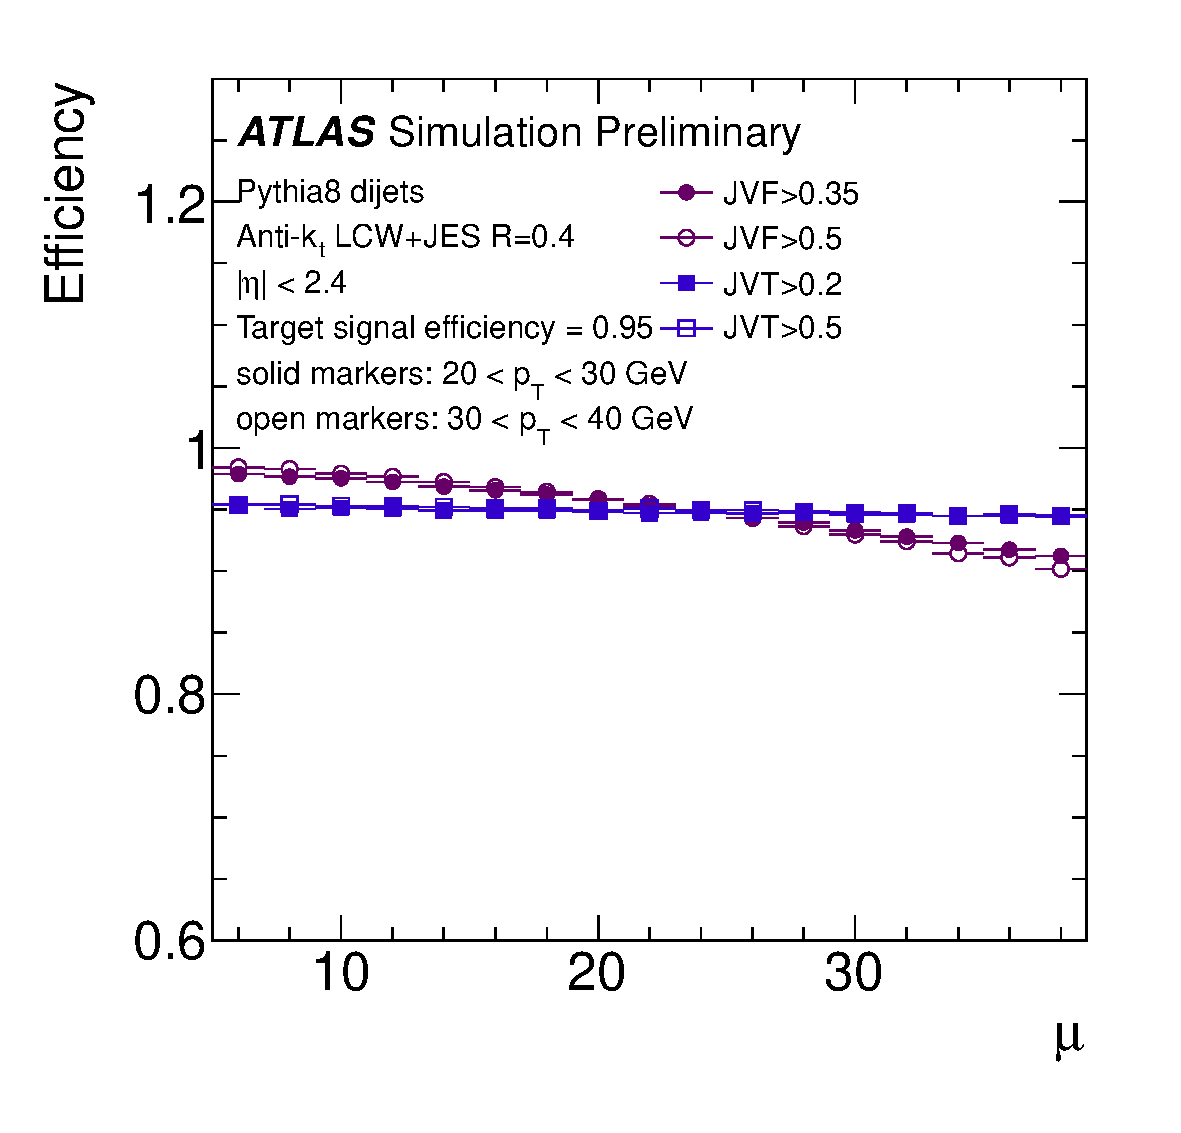
\includegraphics[width=.8\linewidth]{jvt_jvf}
    \caption{Dependence of the hard scatter jet efficiency as a function of the
      average number of interactions per bunch crossing $\nu$. The solid markers
    refers to jets with $20~<~\pt~<30$~GeV while the open markers to jets with
    $30~<~\pt~<40$~GeV. Fixed cuts on JVT (blue) and JVF (purple) are imposed
    such that the inclusive efficiency is 95\%~\cite{JVT}.}
    \label{fig:jvt_jvf}
\end{figure}
%%% Local Variables:
%%% mode: latex
%%% TeX-master: "../search_for_DM_LED_with_ATLAS"
%%% End:


\subsection{Jet Calibration}
\label{sec:jet-calibration}

The \gls{jes} relates the energy measured by the ATLAS detector to the kinematic
properties of the corresponding stable particles, this calibration must take
into account the detector effects such as the non compensating nature of the
ATLAS hadronic calorimeter (see Section~\ref{sec:hadronic-shower}), energy loss
due to inactive regions in the detector or particle showers not fully contained
in the calorimeter. The \emph{electromagnetic scale} is the baseline signal
scale of the ATLAS calorimeters it is established during test beam measurements
with electrons and it accounts correctly for the energy deposited by
electromagnetic showers. The basic jet calibration scheme, applies JES
correction to the EM scale and is usually referred to as EM+JES. The \gls{lcw}
is another calibration method that clusters topologically connected cells,
classifying them as electromagnetic or hadronic and deriving the energy
corrections from single pion MC simulation and dedicated studies to account for
the detector effects, the jets calibrated with this method are referred to as
LCW+JES\@. The \gls{gcw} calibration uses the fact that electromagnetic and
hadronic showers leave a different energy deposition in the calorimeter cells,
with the electromagnetic shower more compact than the hadronic one. The energy
correction are then derived for each calorimeter cell within the jet and
minimizing the energy resolution. The \gls{gs} method starts from EM+JES
calibrated jets and corrects for the fluctuation in particle content of the
hadronic shower using the topology of the energy deposits. The corrections are
applied in a way that leaves unchanged the mean jet energy~\cite{JetCalib}.
%%% Local Variables:
%%% mode: latex
%%% TeX-master: "../search_for_DM_LED_with_ATLAS"
%%% End:


\subsection{Jet Selection}
\label{sec:jet-selection}

In order to distinguish jets coming from $pp$ collisions from those from a
non--collision origin, two jet selection criteria, \emph{loose} and \emph{tight},
are available. The loose selection criteria, provides an efficiency for
selecting jets coming from $pp$ collisions above 99.5\% for $\pt > 20$~GeV, the
tight criteria can reject even further background jets~\cite{JetEff}.

In this analysis the jets are reconstructed using the $\antikt$ algorithm with
the radius parameter R = 0.4. The \emph{baseline jets} are required to have
$|\eta| < 2.8$ and to make sure they come from a HS vertex, they need to satisfy
any of the following:
\begin{enumerate}[A -]
  \item The $\pt > 50$~GeV.
  \item They have $20 < \pt < 50$~GeV and $|\eta| > 2.4$.
  \item They have $20 < \pt < 50$~GeV, $|\eta| < 2.4$ and JVT > 0.64.
\end{enumerate}
Furthermore, events in which the jets, after the overlap removal is applied,
fail the loose selection criteria are disregarded. Finally the most energetic
jet in the event (the \emph{leading jet}) is required to pass the tight
selection criteria. The \emph{good jets} require an increased $\pt$ threshold of
30~GeV and at most 4 HS jet in the event.

In the 2016 analysis the A, B and C conditions above are replaced with:
\begin{enumerate}[D -]
\item $\pt$ > 30~GeV and $|\eta| < 2.8$.
\item $\pt$ > 60~GeV or $|\eta| > 2.4$ or JVT> 0.59.
\end{enumerate}
The selection criteria for both analyses are summarized in \cref{tab:jet_def}.
\begin{table}[!h]
  \centering
  \begin{tabular}{ll}
    \toprule
    \multicolumn{2}{c}{Jet Definition} \\
    \midrule \midrule
    \textbf{Baseline jet} & \textbf{Good jet} \\
    \midrule
    R = 0.4 & \emph{baseline} \\
    $|\eta| < 2.8$ & at most 4 jets \\
    \emph{Loose} selection criteria & $\pt > 30$~GeV (2015) \\
    \emph{Tight} on the leading jet & \\
    passes the overlap removal & \\
    any of (2015): \\
    \tabitem $\pt > 50$~GeV \\
    \tabitem $20 < \pt < 50$~GeV, $|\eta| > 2.4$ \\
    \tabitem $20 < \pt < 50$~GeV, $|\eta| < 2.4$, JVT > 0.64 & \\
    any of (2016): \\
    \tabitem $\pt$ > 30~GeV and $|\eta| < 2.8$ \\
    \tabitem $\pt$ > 60~GeV or $|\eta| > 2.4$ or JVT> 0.59 \\
    \bottomrule
  \end{tabular}
  \caption{Jet definition in the monojet analysis. The year in parentheses
    refers to the selection applied in different versions of the analysis.}
  \label{tab:jet_def}
\end{table}
%%% Local Variables:
%%% mode: latex
%%% TeX-master: "../search_for_DM_LED_with_ATLAS"
%%% End:


\section{Overlap Removal}
\label{sec:overlap-removal}

During object reconstruction, it may happen that different algorithms identify
the same track and cluster as different types of particles, this results in a
duplicate object. In physics analyses a decision must be made on which
interpretation to give to the reconstructed object, this process is called
\gls{or}~\cite{Alison:1536507}.

In this analysis, an overlap removal is applied to electrons, muons and jets
that pass the baseline criteria and the following objects are removed:
\begin{itemize}
\item Remove jet in case any pair of jet and electron satisfies $\Delta R(j,
  e) < 0.2$.
\item Remove electron in case any pair of jet and electron satisfies $0.2 <
  \Delta R(j, e) < 0.4$.
\item Remove muon in case any pair of muon and jet with at least 3 tracks
  satisfies $\Delta R(j, \mu) < 0.4$.
\item Remove jet if any pair of muon and jet with less than 3 tracks satisfies
  $\Delta~R(j, \mu)~<~0.4$.
\end{itemize}
%%% Local Variables:
%%% mode: latex
%%% TeX-master: "../search_for_DM_LED_with_ATLAS"
%%% End:


\section{Missing Transverse Energy}
\label{sec:miss-transv-energy}

Due to the conservation of momentum and the fact that the proton bunches are
parallel to the $z$-axis, the sum of the momenta of the collision products in
the transverse plane should sum to zero. Any energy imbalance is known as
\gls{met}, it may indicate weakly interacting stable particles (neutrinos within
the SM, new particles in beyond SM models) or non reconstructed physical objects
that escape the detector acceptance like for example a muon that goes into a
hole of the muon system (e.g.\ supports for ATLAS) cannot be detected and give
rise to fake $\met$.  Physical objects that are fully reconstructed and
calibrated such as electrons, photons, hadronically decaying tau-leptons, jets
or muons are called \emph{hard objects} and are used to compute the missing
transverse momentum in an event~\cite{MET}. The $x$ and $y$ components of the
$\met$ can be written as:
\begin{equation}
  \label{eq:94}
  E_\mathrm{\, x(y)}^\mathrm{\, miss} = E_\mathrm{\, x(y)}^\mathrm{\, miss,\, e} +
  E_\mathrm{\, x(y)}^\mathrm{\, miss,\, \gamma} + E_\mathrm{\, x(y)}^\mathrm{\,
    miss,\, \tau} + E_\mathrm{\, x(y)}^\mathrm{\, miss,\, \text{jets}} +
  E_\mathrm{\, x(y)}^\mathrm{\, miss,\, \mu} + E_\mathrm{\, x(y)}^\mathrm{\, miss,\,
    \text{soft}}
\end{equation}
where the terms for jets, charged leptons and photons are the negative sum of
the momenta of the respective calibrated object while the \emph{soft term} is
reconstructed from the transverse momentum deposited in the detector that is not
already associated to hard objects. It may be reconstructed by means of
calorimeter-based methods, the so called \gls{cst}, or using track-based methods
known as \gls{tst}.

The CST is reconstructed using energy deposits in the calorimeters which are not
associated to hard objects, it arise from soft radiation accompanying the hard
scatter event and from underlying event activity. A downside of the CST is its
vulnerability to pile up.

The TST is built from tracks not associated to any hard object, tracks can be
associated to vertices and thus to a particular $pp$ collision, making this
method robust against pile-up. This method is, however, insensitive to soft
terms coming from neutral particles that do not leave a track in the ID, thus
the TST $\met$ is combined with calorimeter-based measurements for hard objects.

Due to its stability against pile-up, this analysis uses the TST $\met$ term.
Moreover, the muons are treated as invisible particles in the $\met$
reconstruction (i.e. $E_\mathrm{\, x(y)}^\mathrm{\, miss,\, \mu} = 0$).
%%% Local Variables:
%%% mode: latex
%%% TeX-master: "../search_for_DM_LED_with_ATLAS"
%%% End:


\chapter{The 2015 Monojet Analysis}
\label{cha:monojet-signature}

\section{Motivation}
\label{sec:motivation}

There are two possible cases that results in an energy imbalance in the
detector, the first one occurs in beyond Standard Model physics, that involves
the presence of particles that interact weakly or not at all with normal
matter. These particles are not detected thus leaving an energy imbalance in the
detector. In the second case, the decay products in the final state involve
neutrinos that are not detectable by ATLAS\@. To better understand the second
category of events, consider \cref{fig:susy_standard} that shows the decay
topology of squark pair production with a neutralino and two jets in the final
state. Using the two body decay energy and momentum relations~\cite{PDG}:
\begin{equation}
  \label{eq:95}
  E_q = \frac{M_{\, \tilde{q}}^2 - m_{\, \tilde{\chi}_{\, 1}^{\, 0}}^2 + m_q^2}{2
    M_{\, \tilde{q}}},
\end{equation}
\begin{equation}
  \label{eq:96}
  |\vec{p}_q| = |\vec{p}_{\, \tilde{\chi}_{\, 1}^{\, 0}}| = \frac{\left[ \left(
        M_{\, \tilde{q}}^2 - (m_q + m_{\, \tilde{\chi}_{\, 1}^{\, 0}})^2
      \right) \left( M_{\, \tilde{q}}^2 - (m_q - m_{\, \tilde{\chi}_{\, 1}^{\,
            0}})^2 \right) \right]^{1/2}}{2 M_{\, \tilde{q}}}
\end{equation}
where $M_{\, \tilde{q}}$ is the squark center of mass energy,
$m_{\, \tilde{\chi}_{\, 1}^{\, 0}}$ is the neutralino mass and $m_q$ is the
quark mass. Neglecting the quark mass ($m_q = 0$) we get that:
\begin{equation}
  \label{eq:97}
  E_q = \frac{M_{\, \tilde{q}}^2 - m_{\, \tilde{\chi}_{\, 1}^{\, 0}}^2}{2 M_{\,
      \tilde{q}}},
\end{equation}
\begin{equation}
  \label{eq:98}
  |\vec{p}_q| = |\vec{p}_{\, \tilde{\chi}_{\, 1}^{\, 0}}| = \frac{M_{\,
      \tilde{q}}^2 - m_{\, \tilde{\chi}_{\, 1}^{\, 0}}^2}{2 M_{\, \tilde{q}}}.
\end{equation}
The quark will hadronize in the calorimeter and give rise to a jet that can be
detected by the ATLAS detector only if $\pt > 20$~GeV. If for example the mass
of the squark is $M_{\, \tilde{q}} = 450$~GeV and the mass of the neutralino is
$m_{\, \tilde{\chi}_{\, 1}^{\, 0}} = 445$~GeV then it can be seen from
\cref{eq:98} that the quark and neutralino momenta are given by
$|\vec{p}_q|~=~|\vec{p}_{\, \tilde{\chi}_{\, 1}^{\, 0}}|~\simeq~5$~GeV. Since
the neutralino escape detection, this results in low $\met$ thus when the mass
of the neutralino approaches the mass of the quark this results in a low energy
jet and $\met$. Since the missing energy resolution of the \gls{atlas} detector
is approximately 12~GeV as can be seen from \cref{fig:met_resolution}, such
events cannot be used to trigger and select the event by the \gls{atlas}
detector. This means that there is no sensitivity to \gls{susy} models with
compressed mass spectra (when the mass difference between the particles is
small). This problem applies to many channels of \gls{susy} productions.
\begin{figure}[!h]
  \centering
  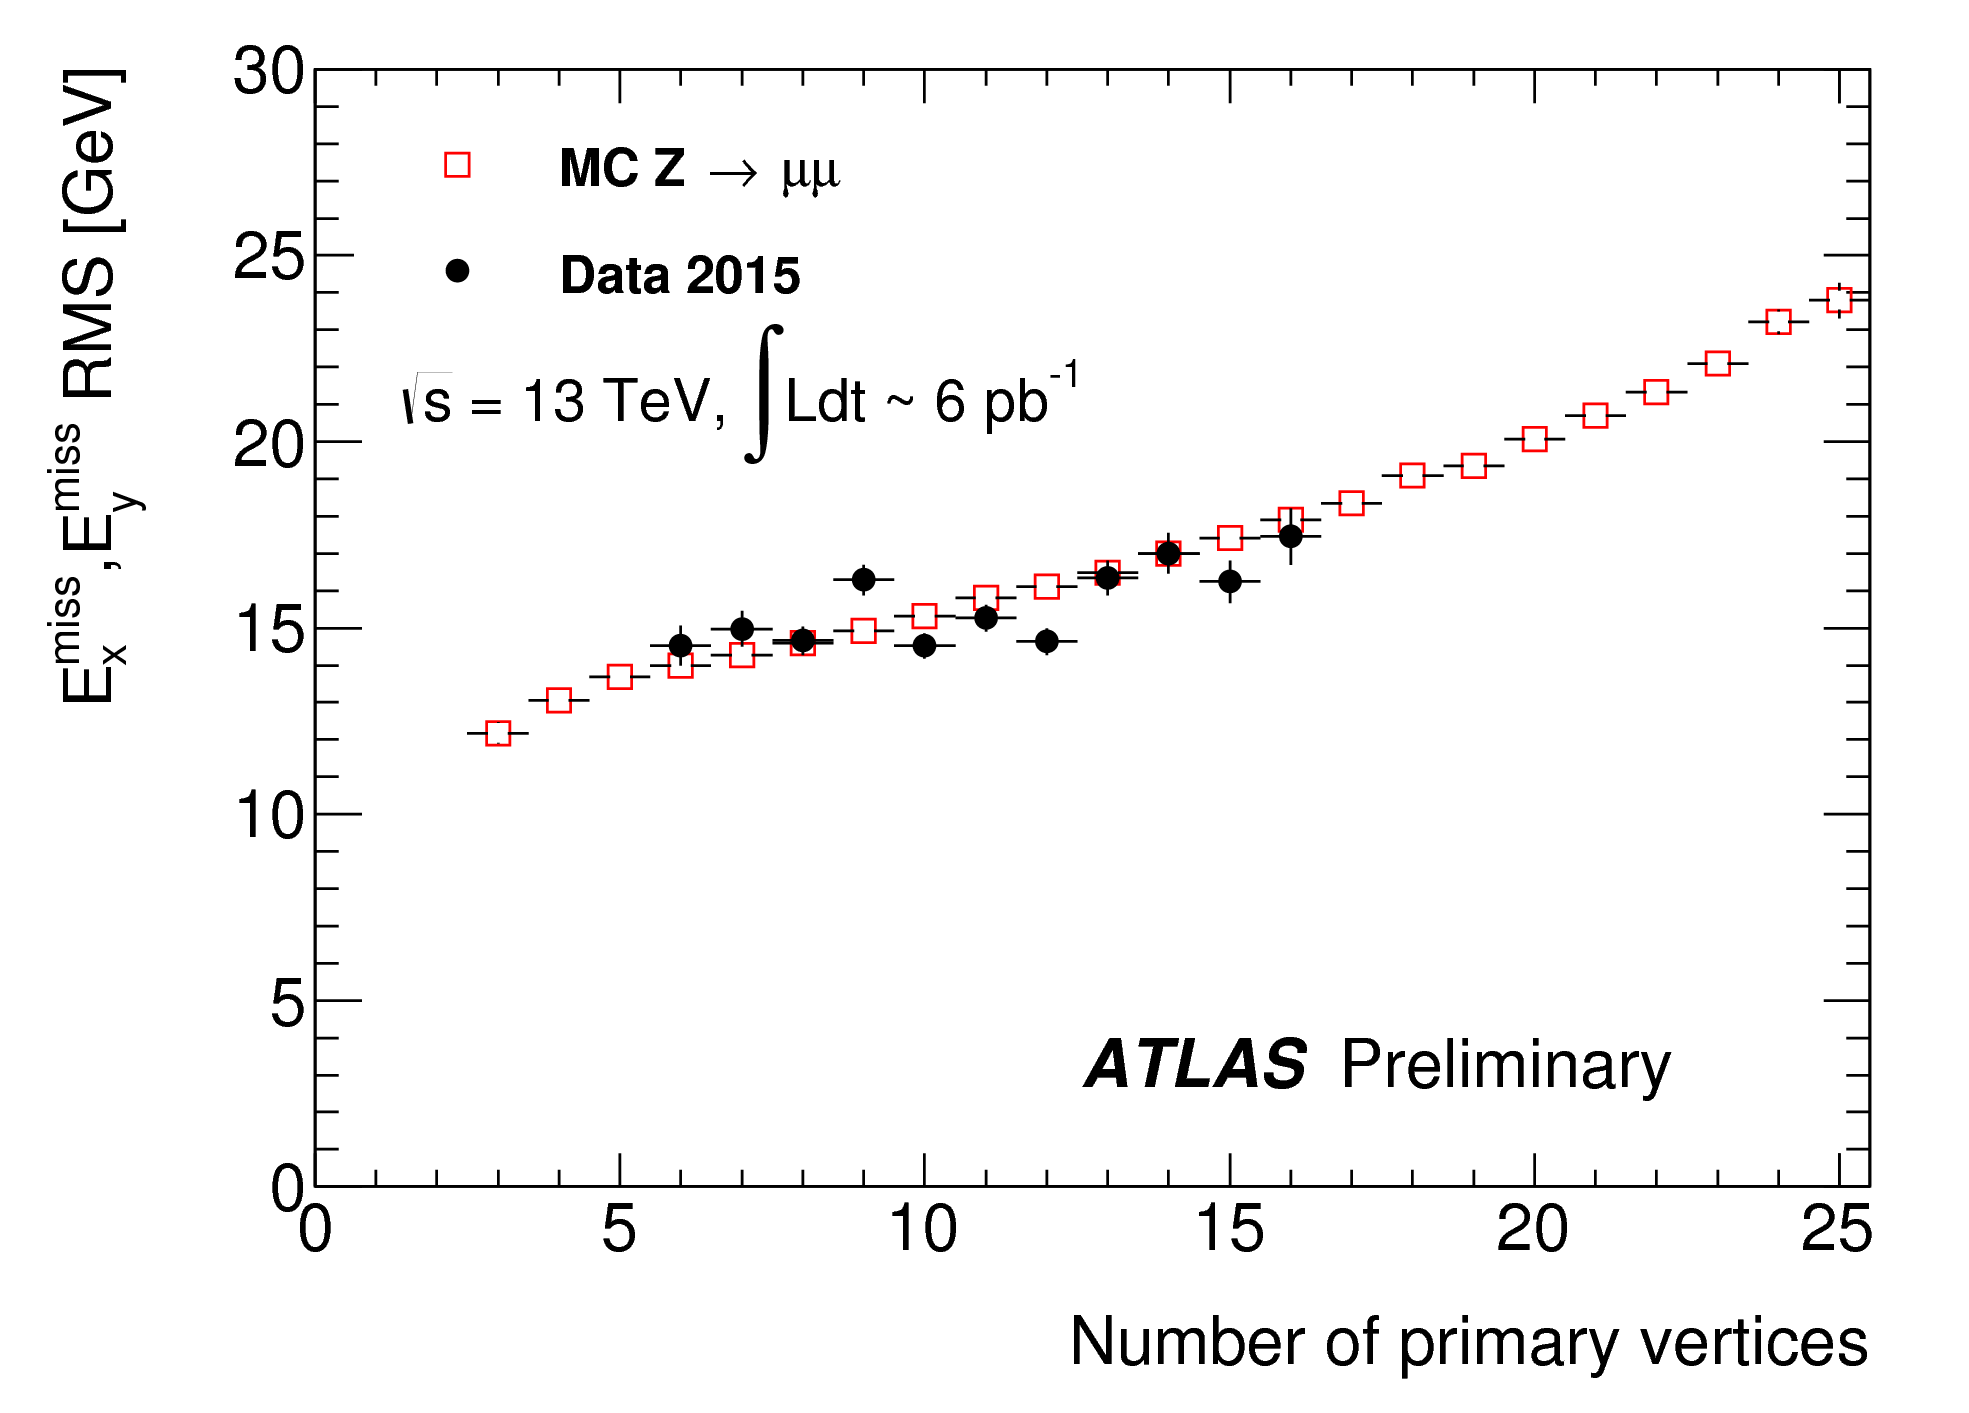
\includegraphics[width=\textwidth]{met_resolution}
  \caption{Distribution of the $x$ and $y$ components of the \gls{tst} $\met$
    resolution as a function of the $\sum E_\mathrm{\, T}$ and of the number of
    primary vertexes in $\zmumuplusjets$ events~\cite{METResolution}.}
  \label{fig:met_resolution}
\end{figure}

\cref{fig:susy_exclusion} shows this effect for the search for squark pair
production in the case of the squark decaying directly to a quark and a
neutralino through the mechanism illustrated in \cref{fig:susy_standard}. This
search uses a classical multijet + $\met$ analysis, it can be seen that there is
no sensitivity close to the diagonal (dashed line) in the region
$400~<~M_{\, \tilde{q}}~<~600$~GeV.

If an initial state radiation jet is present in the event, as depicted in
\cref{fig:susy_compressed}, the squark-squark system gets boosted in the
opposite direction thus increasing the momentum of the decay products and the
missing energy leading to a signature of a high $\pt$ jet on one side and
additional jets and $\met$ on the other side of the event.

Events with an energetic jet $\pt$ and large $\met$ in the final state
constitute a clean signature for new physics searches at hadron colliders.
Signals that can be studied with this experimental signature include the
production of \glspl{wimp}, the \gls{add} model for large extra dimensions and
\gls{susy}.
\begin{figure}[!h]
  \centering
  \begin{subfigure}[t]{.48\linewidth}
    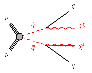
\includegraphics[width=\linewidth]{susy_standard}
    \caption{Event without initial state radiation~\cite{SUSYPub}.}
    \label{fig:susy_standard}
  \end{subfigure} \quad
  \begin{subfigure}[t]{.48\linewidth}
    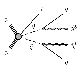
\includegraphics[width=\linewidth]{compressed}
    \caption{Event with initial state radiation~\cite{ExotPub}.}
    \label{fig:susy_compressed}
  \end{subfigure}
  \caption{Event topology of squark pair production resulting in a neutralinos
    with two jets final state with (\cref{fig:susy_compressed}) and without
    (\cref{fig:susy_standard}) initial state radiation.}
  \label{fig:motivation}
\end{figure}
\begin{figure}[!h]
  \centering
  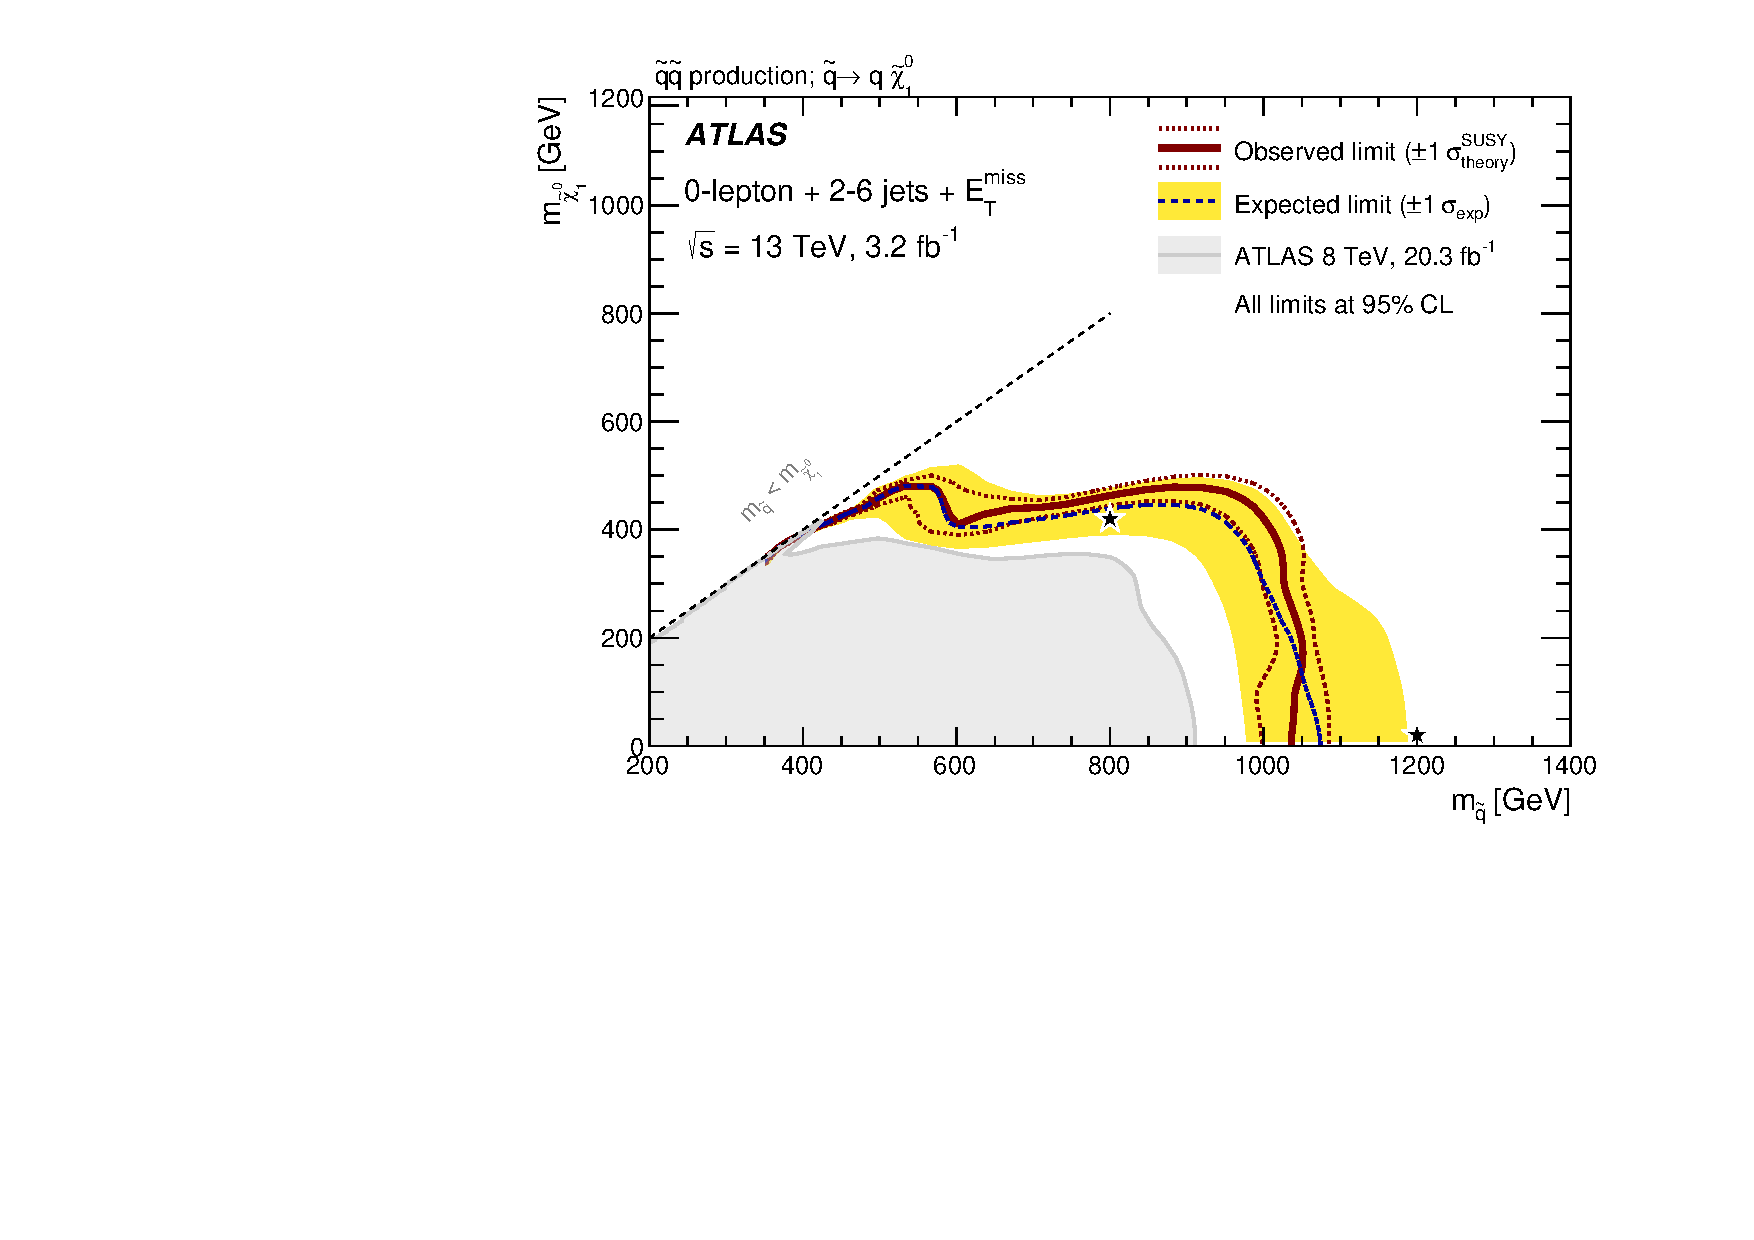
\includegraphics[width=\linewidth]{susy}
  \caption{Exclusion limits for direct production of squark
    pairs where the squark decays into a quark and a neutralino. The $x$-axis
    represents the mass of the squark and the $y$-axis represents the mass of
    the lightest neutralino. The black stars represent a benchmark model as
    explained in more details in Ref.~~\cite{SUSYPub}.}
  \label{fig:susy_exclusion}
\end{figure}
%%% Local Variables:
%%% mode: latex
%%% TeX-master: "../search_for_DM_LED_with_ATLAS"
%%% End:


\section{Event Selection}
\label{sec:event-selection}

The search for squark pair production with compressed mass spectrum is carried
out in $pp$ collisions using the data collected by the ATLAS experiment during
the 2015 Run II corresponding to a total integrated luminosity of 3.2 \ifb. The
signal region is defined by the following selection criteria:
\begin{enumerate}[A -]
\item The HLT\_xe70 trigger was used in the whole 2015 dataset.
\item In order to assure that the event originated from a $pp$ collision, a
  primary vertex with at least two associated tracks with $\pt > 0.4$~GeV is
  required.
\item Events in which any jet fails the \emph{loose} jet cleaning criteria are
  rejected. This suppress noise from non-collision background.
\item The most energetic jet in the event (the \emph{leading jet}) must have
  $\pt > 250~$GeV and $|\eta| < 2.4$. Moreover, in order to reject beam-induced
  and cosmic particles background, the event is rejected if the leading jet
  fails the \emph{tight} cleaning criteria.
\item In order to suppresses $Z (\rightarrow \ell \bar{\ell})$ + jets and
  $W (\rightarrow \ell \nu)$ background, events with an identified electron of
  $\pt > 20~$GeV or muon of $\pt > 10~$GeV are rejected, see
  \cref{sec:electrons,sec:muons} for the lepton definitions.
\item In order not to overlap with other ATLAS SUSY searches, events with more
  than four jets are rejected, see \cref{sec:jet-veto} for more details on this
  selection.
\item The $\met$ trigger can select multi-jet events in case of a
  mis--reconstructed jet. In these cases the missing transverse momentum points
  in the direction of one of the jets, this background can be suppressed by
  imposing a minimum azimuthal angle separation between the missing transverse
  momentum and any jet of $\Delta \phi (\mathrm{jets}, \met) > 0.4$.
\item A $\met > 250~$GeV requirement is imposed in order to be able to test
  different BSM signals with different sensitivities to the missing energy.
\item Events with an identified electron of $\pt > 20~$GeV or muon of
  $\pt > 10~$GeV are vetoed in order to suppress the
  $Z (\rightarrow \ell \bar{\ell})$ + jets and $W (\rightarrow \ell \nu)$
  background. See \cref{sec:electrons,sec:muons} for the lepton definitions.
\end{enumerate}
Inclusive (IM1--IM7) and exclusive (EM1--EM6) \glspl{sr} are defined in the
monojet analysis with increasing $\met$ thresholds from 250~GeV to 700~GeV, see
Table~\ref{tab:event_selection} for the exact definition of the signal
regions. These different $\met$ bins are defined in order to address different
BSM signals tested with the monojet signature. In this chapter special emphasis
is placed on the compressed squark-neutralino model.
\begin{table}[!th]
  \centering
  % The @{} is to avoid extra horizontal space
  \begin{tabular}{@{}l@{}c@{}c@{}c@{}c@{}c@{}c@{}c}
    \toprule
    \multicolumn{8}{c}{Event Selection Criteria} \\
    \midrule \midrule
    \multicolumn{8}{l}{HLT\_xe70 trigger} \\
    \multicolumn{8}{l}{Primary Vertex} \\
    \multicolumn{8}{l}{$\met > 250~$GeV} \\
    \multicolumn{8}{l}{Leading jet with $\pt > 250~$GeV and $|\eta| < 2.4$} \\
    \multicolumn{8}{l}{At most 4 jets} \\
    \multicolumn{8}{l}{$\Delta \phi (\mathrm{jets}, \met) > 0.4$} \\
    \multicolumn{8}{l}{Jet quality requirements} \\
    \multicolumn{8}{l}{No identified muon with $\pt > 10~$GeV or electron of
    $\pt > 20~$GeV} \\
    \midrule
    Inclusive SRs & IM1 & IM2 & IM3 & IM4 & IM5 & IM6 & IM7 \\
    $\met$~[GeV] & > 250 & > 300 & > 350 & > 400 & > 500 & > 600 & > 700 \\
    \midrule
    Exclusive SRs & EM1 & EM2 & EM3 & EM4 & EM5 & EM6 \\
    $\met$~[GeV] & [250--300] & [300--350] & [350--400] & [400--500] &
    [500--600] & [600--700] \\
    \bottomrule
  \end{tabular}
  \caption{Definition of the signal region.}
  \label{tab:event_selection}
\end{table}
%%% Local Variables:
%%% mode: latex
%%% TeX-master: "../search_for_DM_LED_with_ATLAS"
%%% End:


\section{Jet Veto }
\label{sec:jet-veto}

In order to reduce the overlap with other \gls{atlas} data analyses, especially
those containing multijet final states, an upper cut on the number of \gls{hs}
jets is necessary. This procedure is denominated \emph{jet veto}. In order to
define hard scatter jets, cuts on the jet $\pt$ and on the \gls{jvt} (see
\cref{sec:jet-vertex-tagger}) have been studied. The aim of these cuts is to
render the analysis independent from pile-up as much as possible but stay signal
efficient, too hard cuts would lead to disregarding possible signal events
while, on the other hand, too loose cuts let pile-up jets in the signal region
and allow significant overlap with other \gls{atlas} searches.

Due to the jets coming from the squark decays, the \gls{susy} compressed
squark-neutralino model has more jets compared to other signals considered in
the monojet analysis and are therefore the most sensitive to jet veto efficiency
and to the definition of hard scatter jet. To study the pile-up contamination
for different $\pt$ thresholds a \emph{figure of merit} is defined and its
dependence from the average number of proton-proton collisions per bunch
crossing studied. The figure of merit is referred to as \emph{jet veto
  efficiency } and defined as:
\begin{equation}
  \label{eq:fig_merit}
  \frac{\text{N (events) with baseline cuts + at
      most N (jet) HS jets}}{\text{N (events)
      with baseline cuts}}
\end{equation}
where the baseline cuts are the event selection given in
\cref{sec:event-selection} except the cut F (the study presented here uses a
symmetric $\met$ and leading jet $\pt$ cut at 250~GeV) and the hard scatter jets
are defined as:
\begin{itemize}
\item Jets with $\pt > 50$ GeV is always considered coming from the hard
  scatter.
\item Due to the lacking of a tracking system in the $|\eta| > 2.4$ region and
  thus the impossibility of using a \gls{jvt} criteria, jets belonging to the
  $|\eta| > 2.4$ (forward jets) are always considered as coming from the hard
  scatter.
\item In order to be considered coming from the hard scatter proton-proton
  collision, the jets with $\pt^{\mathrm{thresh}} < \pt < 50$~GeV must
  additionally satisfy a
  $\mathrm{\gls{jvt}}~>~\mathrm{\gls{jvt}}^{\text{ thresh}}$ selection criteria
  where different $\pt^{\mathrm{thresh}}$ and \gls{jvt}$^{\mathrm{\, thresh}}$
  are studied, in particular:
  \begin{enumerate}[A -]
  \item
    $\pt^{\mathrm{thresh}} \in
    \{30~\mathrm{GeV},~40~\mathrm{GeV},~50~\mathrm{GeV}, ~70~\mathrm{GeV}\}$,
  \item \gls{jvt}$^{\mathrm{\, thresh}}~\in~ \{0.14,~0.64,~0.92\}$.
  \end{enumerate}
\end{itemize}

As can be seen from \cref{fig:susy_compressed}, at least three jets in the event
are required for the \gls{susy} compressed spectra models, on the other hand
other searches~\cite{MultijetSUSY} already explore signatures with four jets or
more. For these reasons and to increase the acceptance of the \gls{susy}
compressed models, events with at most three or four jets are studied with
different $\pt$ thresholds.  \cref{fig:comp_4jets_nojvt,fig:comp_3jets_nojvt}
shows the jet veto efficiency for the different values of
$\pt^{\mathrm{\, thresh}}$ and number of jets in the case where no \gls{jvt} cut
is applied. With a maximum number of jets of three 30~GeV jets the signal
efficiency loss is as large as 20\%. The \gls{jvt} cut reduces the loss of
efficiency for the signal, by preventing pile-up jets to trigger a veto of the
signal events. For three jets at 30~GeV the loss of signal is reduced from about
20\% in \cref{fig:comp_3jets_nojvt} to approximately 15\% in
\cref{fig:comp_3jets_jvt64} and becomes lesser than 5\% for at most four jets.
% \cref{fig:comp_4jets_nojvt} shows the jet veto efficiency for the
% different values of $\pt^{\mathrm{\, thresh}}$ and N~(jets)~$\leq~4$ in the case
% where no JVT cut is applied. In the case of $\pt^{\mathrm{\, thresh}}$ of 30~GeV
% the pile-up dependence is noticeable while it becomes less important with
% tighter cuts. In \cref{fig:comp_4jets_jvt64} a JVT $>$ 0.64 selection is applied
% in the definition of the hard scatter jets, in this case the pile-up dependence
% for the $pt^{\mathrm{\, thresh}}$ of 30~GeV is reduced and the distribution for
% $\pt^{\mathrm{\, thresh}}$ of 40, 50 and 70~GeV cuts is, within statistical
% error, flat.
\begin{figure}[!h]
  \centering
  \begin{subfigure}[t]{.48\linewidth}
    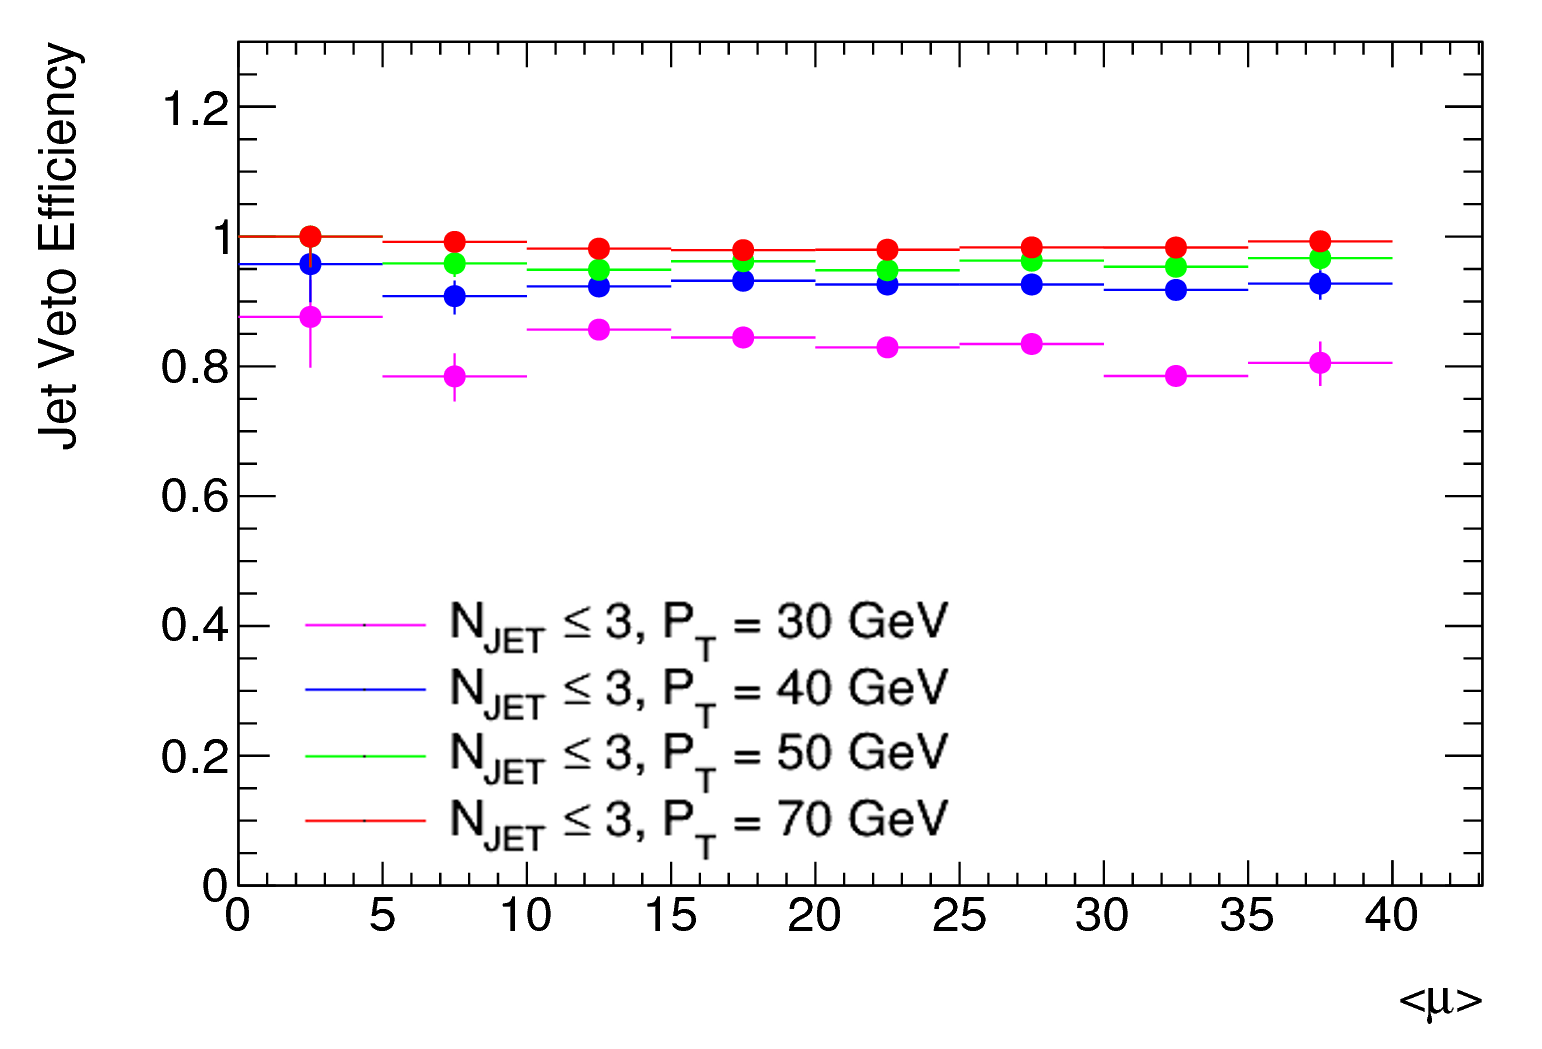
\includegraphics[width=\linewidth]{Compressed_450_435_mu_3jets_M0}
    \caption{No JVT cut applied.}
    \label{fig:comp_3jets_nojvt}
  \end{subfigure}
  \begin{subfigure}[t]{.48\linewidth}
    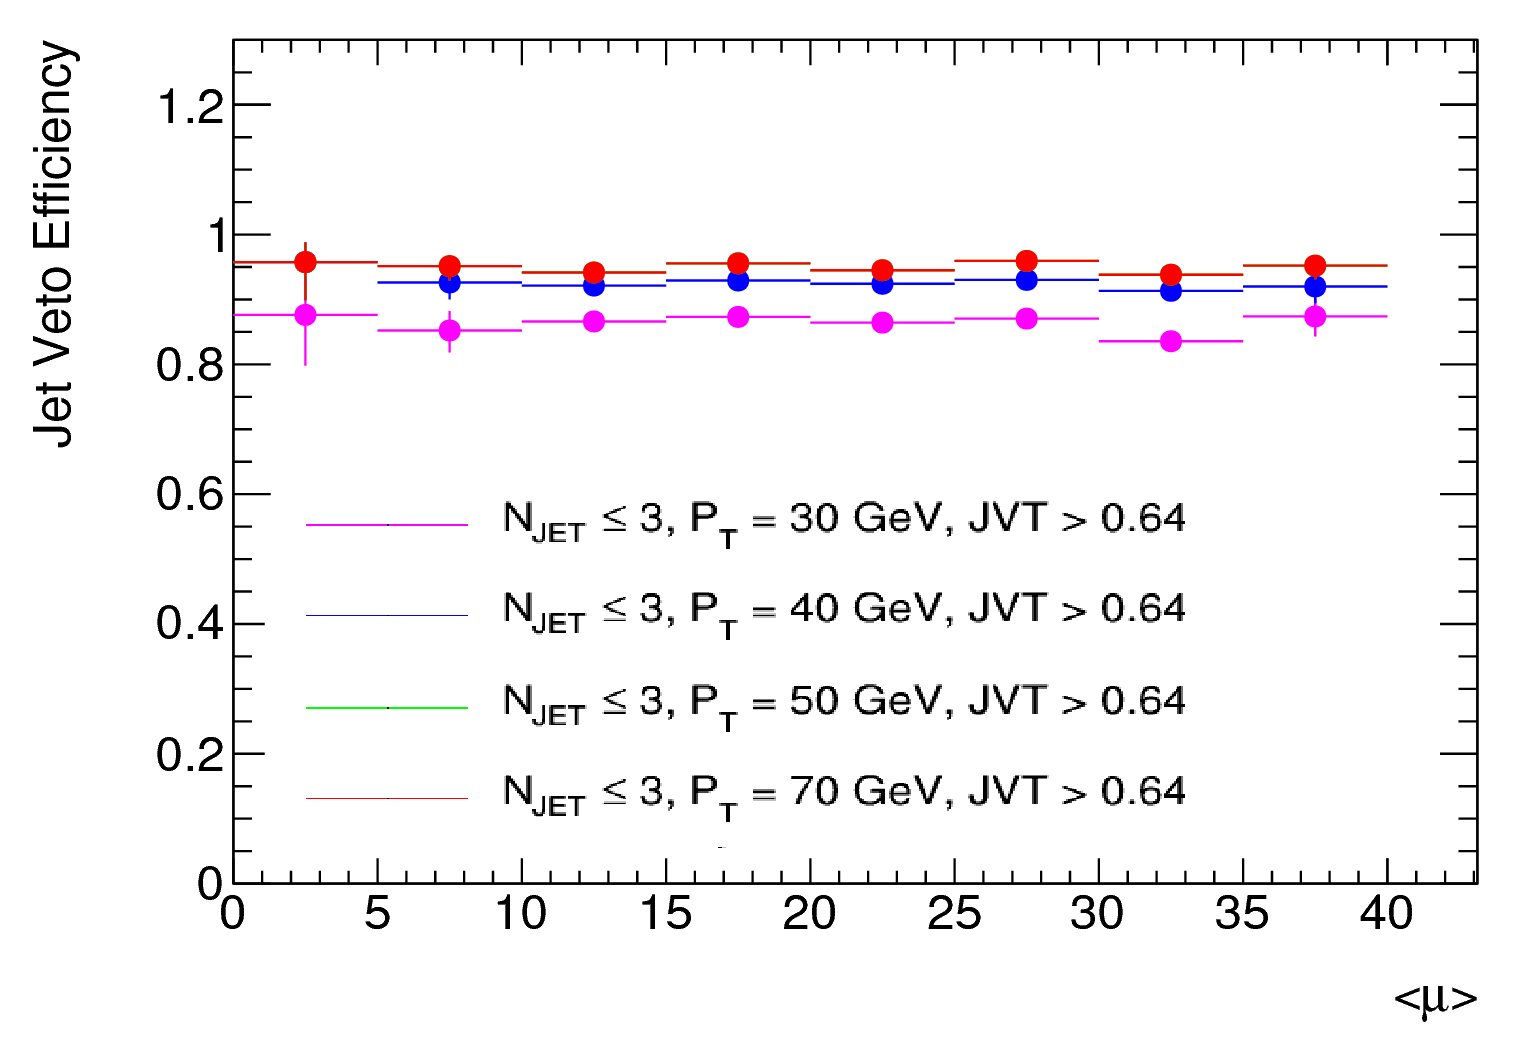
\includegraphics[width=\linewidth]{Compressed_450_435_mu_3jets_jvt64_M0}
    \caption{JVT > 0.64.}
    \label{fig:comp_3jets_jvt64}
  \end{subfigure}
  \begin{subfigure}[t]{.48\linewidth}
    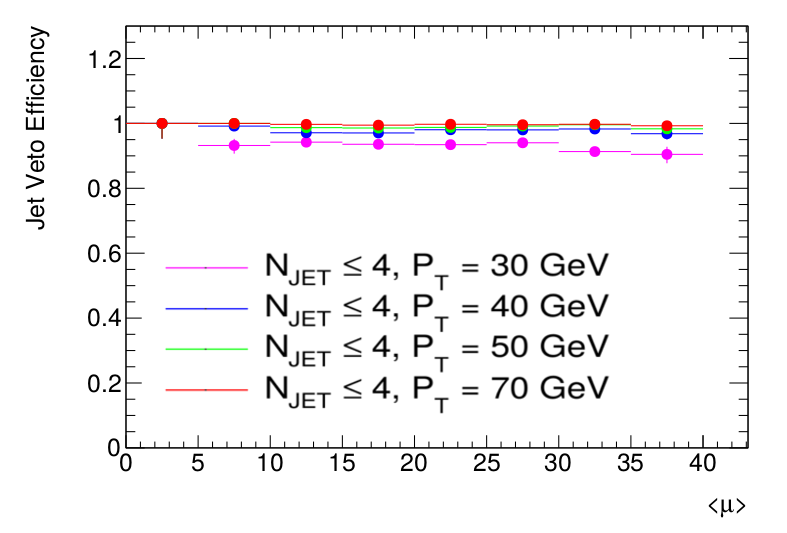
\includegraphics[width=\linewidth]{Compressed_450_435_mu_4jets_M0}
    \caption{No JVT cut applied.}
    \label{fig:comp_4jets_nojvt}
  \end{subfigure}
  \begin{subfigure}[t]{.48\linewidth}
    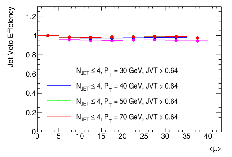
\includegraphics[width=\linewidth]{Compressed_450_435_mu_4jets_jvt64_M0}
    \caption{JVT > 0.64.}
    \label{fig:comp_4jets_jvt64}
  \end{subfigure}
  \caption{Jet veto efficiency for different jet $\pt$ thresholds and number of
    jets as a function of the average number of interactions per bunch crossing
    $\langle \mu \rangle$ for a compressed spectra model point $\msquark = 450$
    GeV $\mneutralino = 435$ GeV. In
    \cref{fig:comp_4jets_nojvt,fig:comp_3jets_nojvt,} no \gls{jvt} cut is
    applied and there is some drop of the efficiency at high pile-up. In
    \cref{fig:comp_4jets_jvt64,fig:comp_3jets_jvt64} a \gls{jvt} $> 0.64$ cut is
    applied, the dependence from pile-up is reduced.}
  \label{fig:comp_eff}
\end{figure}
From this study and similar ones on other signals explored by this analysis, it
was decided to select events with at most four jets above 30~GeV. Even though
harder cuts on the $\pt$ of the jets provide a better efficiency, such a choice
would overlap with the analysis given in Ref.~\cite{MultijetSUSY}.
\cref{fig:jet_veto_comparison} shows the same behavior described above on the
$\znunu$ background. Also in this case an improvement of the jet veto efficiency
as function of the average number of interaction per crossing especially for
$\pt = 30$~GeV is seen. The selected definition of the hard-scatter jets, with N
(jets) $\leq$ 4 is pile-up independent.
\begin{figure}[!h]
  \centering
  \begin{subfigure}[t]{.48\linewidth}
    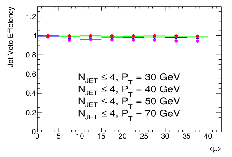
\includegraphics[width=\linewidth]{Znunu_mu_4jets_M0}
    \caption{No JVT cut applied.}
    \label{fig:znunu_4jets_jvt64}
  \end{subfigure}
  \begin{subfigure}[t]{.48\linewidth}
    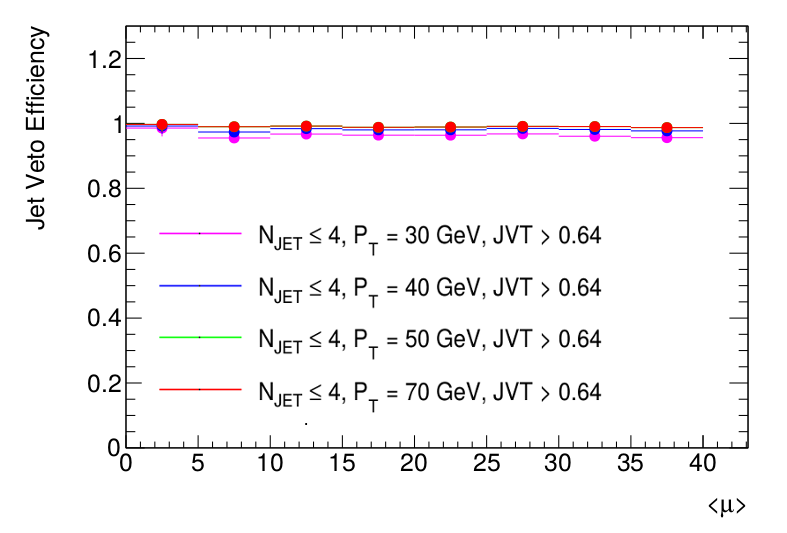
\includegraphics[width=\linewidth]{Znunu_mu_4jets_jvt64_M0}
    \caption{JVT > 0.64.}
    \label{fig:comp_4jets_jvt64_1}
  \end{subfigure}
  \caption{Jet veto efficiency for different jet $\pt$ thresholds and N (jets)
    $\leq 4$ as a function of the average number of interactions per bunch
    crossing $\langle \mu \rangle$ for the $\znunu$ background. In
    \cref{fig:comp_4jets_nojvt} no \gls{jvt} cut is applied and there is some
    drop of the efficiency at high pile-up. In \cref{fig:comp_4jets_jvt64} a
    \gls{jvt} $> 0.64$ cut is applied, the dependence from pile-up is reduced.}
  \label{fig:jet_veto_comparison}
\end{figure}
%%% Local Variables:
%%% mode: latex
%%% TeX-master: "../search_for_DM_LED_with_ATLAS"
%%% End:


\section{Sources of Background}
\label{sec:sources-background}

The Standard Model process $\znunu$~+~jets where the neutrinos escape detection
generating large $\met$ is experimentally similar to signal events in the search
for \gls{bsm} physics with a high energy jet and large missing energy signature
in the final state. This process constitutes an irreducible background and is
the largest background in the analysis. The key to estimate the $\znunu$~+~jets
background is to be able to predict the momentum spectrum of the Z boson and,
since this is assumed to be equal to the $\met$, the corresponding amount of
missing transverse energy. The control regions defined in later sections provide
ways to derive the $Z$ boson momentum using data control regions.

The second biggest source of background with a monojet topology is the
$W (\rightarrow \ell \nu)$~+~jets and in particular
$W (\rightarrow \tau \nu)$~+~jets, in which the $\tau$ decays hadronically, it
gives the highest contribution to this class of events. The
$W (\rightarrow \ell \nu)$~+~jets events with $\ell = e$ or $\mu$ can fake a
monojet signature if the lepton escapes the detector acceptance or has a quality
that is lower than the quality of the lepton veto criteria.

Other background processes are di-boson, $t \bar{t}$ and single top
processes. Multi-jet production from \gls{qcd} processes where one or more jets
are mis-reconstructed leading to high $\met$ represent a small source of
background. Finally \gls{ncb} coming from cosmic particles, detector noise and
beam-induced background can give rise to fake jets and consequently to
$\met$. As discussed in more details in the upcoming sections the control
regions will be used to effectively scale the Monte Carlo predictions for the $V$
+ jets processes using normalization factors (see \cref{sec:glob-simult-likel}).
%%% Local Variables:
%%% mode: latex
%%% TeX-master: "../search_for_DM_LED_with_ATLAS"
%%% End:


\section{Estimation of the $Z$ + jets and $W$ + jets backgrounds}
\label{sec:estimation-z-+}

A \gls{cr} is a region of the phase space where the signal contribution is
negligible but the event selections are similar to those of the signal region so
that the normalization of the backgrounds in the signal region can be deduced
from observed number in the control regions. The main reason to define control
regions is to compute and check the agreement in shape and normalization between
MC simulations and data in reconstructed kinematic quantities. The $V$ + jets,
where $V$ is either a $W$ or a $Z$ vector boson, constitutes the main background
of the monojet analysis. The Monte Carlo simulations for the $V$ + jets
processes are generated using SHERPA~\cite{SHERPA} with 0, 1 or 2 jets at
\gls{nlo} and 2 or 4 jets at \gls{lo}. A pure \gls{mc} estimation of these
processes, suffers from theoretical uncertainties like the limited knowledge of
the \glspl{pdf}, limited order accuracy of the Monte Carlo generators and
experimental uncertainties related to the jet energy scale and luminosity
determination. In order to estimate the contribution of these backgrounds in the
SR, a \emph{data driven} technique is used. The method aims at reducing the
systematic uncertainties by relying on information from data in the \glspl{cr}
rather than on \gls{mc} simulations. It can be divided in three major steps:
\begin{itemize}
\item Define CRs to select $V$ + jets event in data.
\item Calculate a transfer factor from MC predicted events in the \gls{cr} to
  background estimates in the \gls{sr}\@.
\item Apply the transfer factor to the observed events in the \gls{cr} to obtain
  the estimate number of events from the process in the \gls{sr}\@.
\end{itemize}
The CRs used to constrain the $V$ + jets backgrounds have an event selection
that differs from the SR only in the lepton veto and the missing transverse
momentum calculation. Owing to the different lepton selections the \glspl{cr}
and \glspl{sr} are orthogonal and a minimum contribution from a monojet-like
signal is expected.
%%% Local Variables:
%%% mode: latex
%%% TeX-master: "../search_for_DM_LED_with_ATLAS"
%%% End:


\subsection{The Muon Control Region}
\label{sec:muon-control-region}

The muon control region ($\crwmn$) is used to estimate the $\wmunuplusjets$ and
the $\znunuplusjets$ background contribution in the SR\@. The $\wmunuplusjets$
events can enter the SR if the muon is outside the detector acceptance or it
fails quality criteria. $\wmunuplusjets$ events are selected and used in order
to estimate the $\znunuplusjets$ contribution in the signal region. The muon is
treated like a neutrino in the $\met$ calculation, in this way the $\met$ is a
measurement of the $W$ momentum which is later translated in the $Z$ boson
momentum to estimate the $\znunuplusjets$ background. In addition to cuts from A
to H defined in \cref{sec:event-selection} the CR$_{\mathrm{\, wmn}}$ region
selects events with:
\begin{itemize}
\item Exactly one good muon.
\item The transverse mass, defined as:
  \begin{equation}
    \label{eq:99}
    m_\mathrm{\, T} = \sqrt{2 p_\mathrm{\, T}^{\, \mu} p_\mathrm{\, T}^{\, \nu}
      (1 - \cos(\phi_\mu - \phi_\nu))}
  \end{equation}
  and determined by the muon $\pt$ ($\pt^{\, \mu}$) and neutrino $\pt$
  ($\pt^{\, \nu}$), is required to be $30~<~m_\mathrm{\, T}~<~100$~GeV,
  consistent with $W$ boson production. The neutrino $\pt$ is calculated
  assuming that $\pt^{\, \nu} = \met$.
\end{itemize}
The transverse mass cut suppress the $\wtaunuplusjets$ processes in this
region. The measured $\met$ and leading jet $\pt$ distributions after the
fitting the background normalizations to the control regions (see
\cref{sec:glob-simult-likel}) are shown in Figure~\ref{fig:muon_cr_plots}. The
agreement between data and MC is good.
\begin{figure}[!h]
  \centering
  \begin{subfigure}[t]{.48\linewidth}
    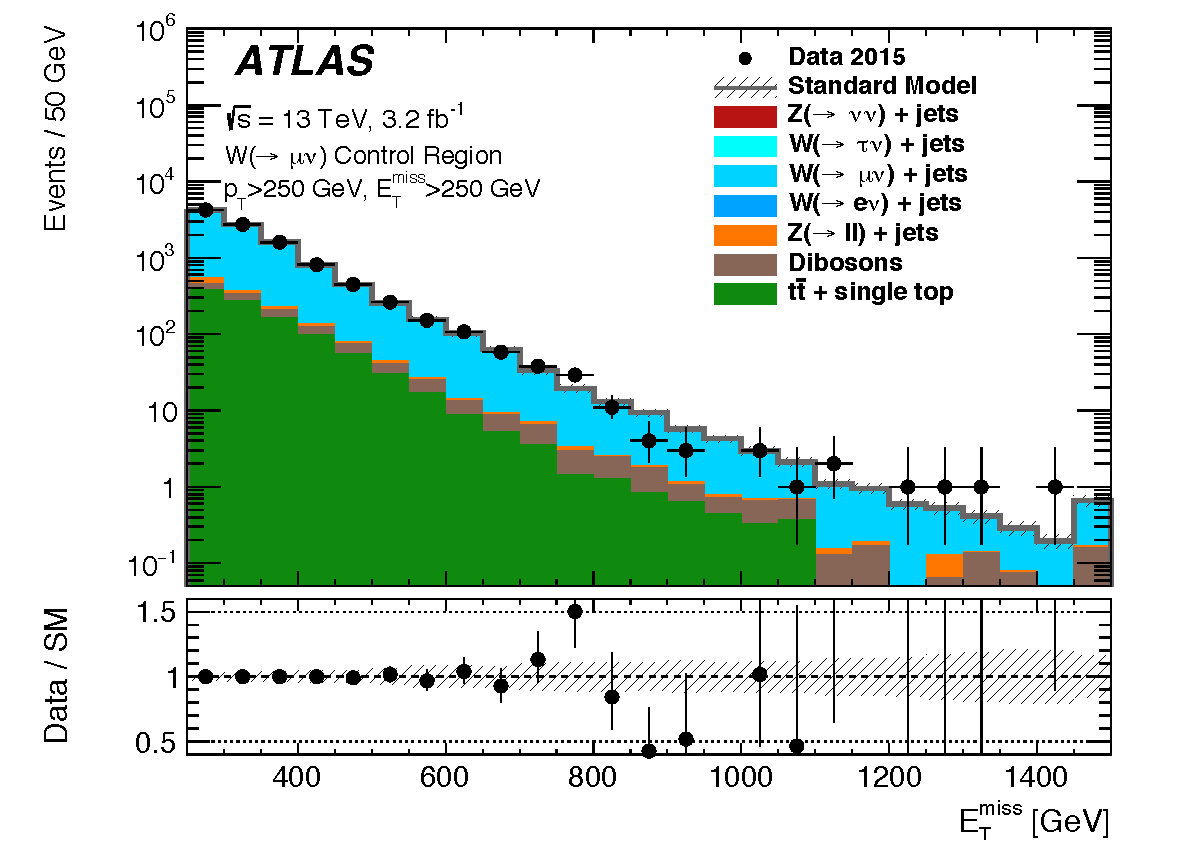
\includegraphics[width=\linewidth]{muon_cr_et_miss_post_fit}
    \caption{$\met$ distribution.}
    \label{fig:muon_cr_et_miss_pre_fit}
  \end{subfigure}
  \begin{subfigure}[t]{.48\linewidth}
    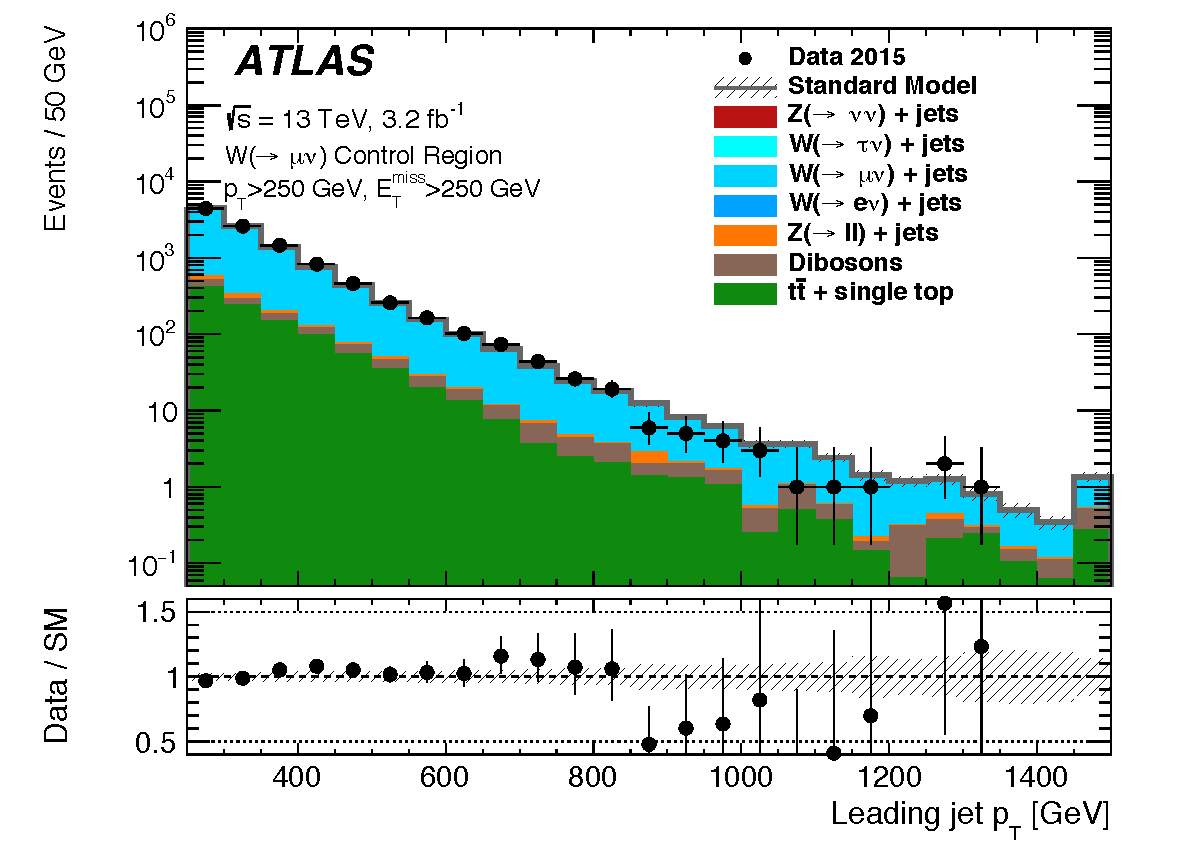
\includegraphics[width=\linewidth]{muon_cr_jet1_pt_post_fit}
    \caption{Leading jet $\pt$ distribution.}
    \label{fig:muon_cr_jet1_pt_pre_fit}
  \end{subfigure}
  \caption{Observed and predicted $\met$ and leading jet $\pt$ distributions
    after the background only fit in the single muon $\crwmn$ for the
    $\met > 250~$GeV selection. The error bands include the statistical and
    systematic error.}
  \label{fig:muon_cr_plots}
\end{figure}
%%% Local Variables:
%%% mode: latex
%%% TeX-master: "../search_for_DM_LED_with_ATLAS"
%%% End:


\subsection{The Electron Control Region}
\label{sec:electr-contr-regi}

The $\wenuplusjets$ process enters the signal region, thus contributing to the
background, in case the electron is not identified in the detector. In the
$\wtaunuplusjets$ process the $\tau$ particle can decay hadronically in 65\% of
the cases resulting in additional jets that can help this background mimic the
signal. To address these backgrounds an electron control region
(CR$_\mathrm{\, ele}$) is built. It is designed to constrain both
$\wenuplusjets$ and $\wtaunuplusjets$ processes thanks to the decays of $\tau$
leptons into electrons. In order to efficiently reject multi-jet background,
the electron is retained in the $\met$ calculation, the missing transverse
momentum in this case measures the momentum of the escaping neutrino. In
addition to cuts from A to H defined in \cref{sec:event-selection} the
CR$_\mathrm{\, ele}$ region selects events with:
\begin{itemize}
\item Exactly one good electron.
\item No additional leptons in the final state.
\end{itemize}
In order to enhance the $\wtaunuplusjets$ contribution in this region, no
$m_\mathrm{\, T}$ cut is applied. \cref{fig:ele_cr_plots} shows the observed and
predicted $\met$ and the leading jet $\pt$ distribution in this control region. The
overall agreement between data and MC is good and improved after the global
likelihood fit procedure described in \cref{sec:glob-simult-likel}.
\begin{figure}[!h]
  \centering
  \begin{subfigure}[t]{.48\linewidth}
    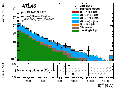
\includegraphics[width=\linewidth]{ele_cr_et_miss_post_fit}
    \caption{$\met$ distribution.}
    \label{fig:ele_cr_et_miss_pre_fit}
  \end{subfigure}
  \begin{subfigure}[t]{.48\linewidth}
    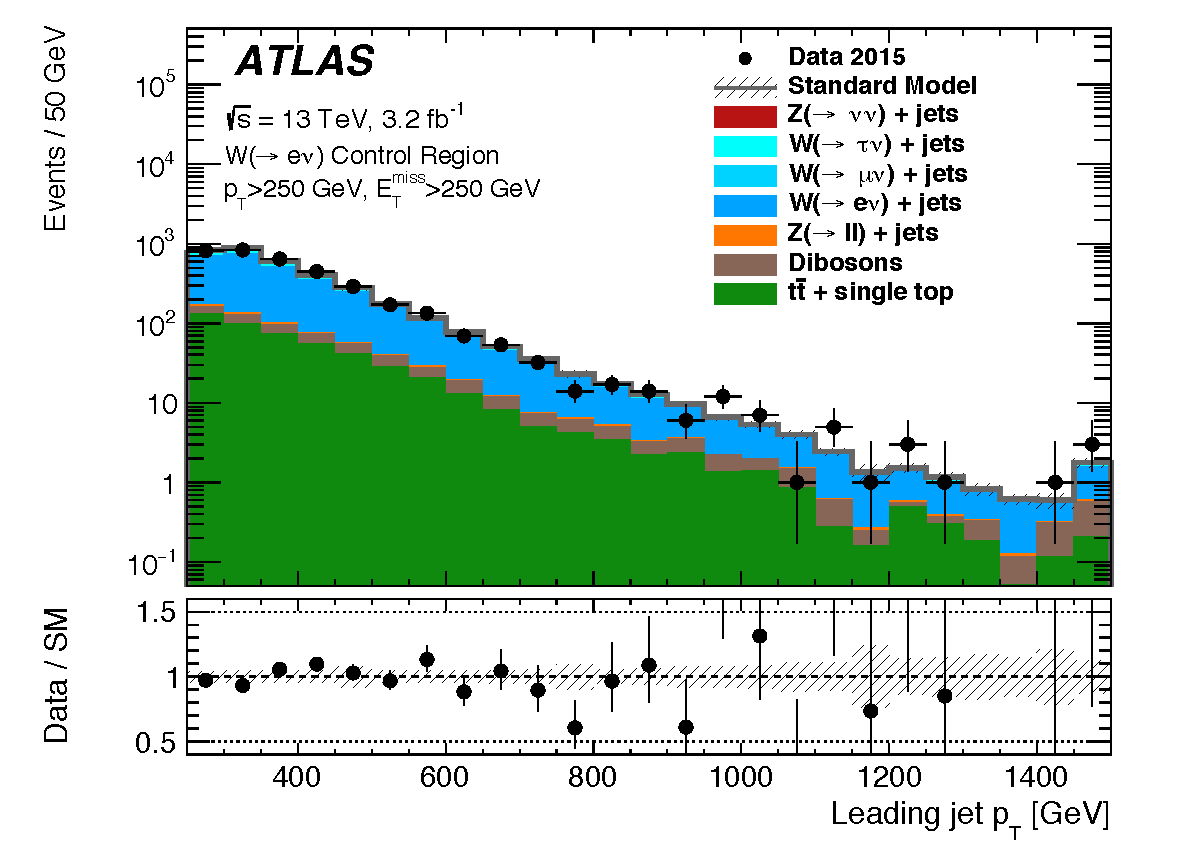
\includegraphics[width=\linewidth]{ele_cr_jet1_pt_post_fit}
    \caption{Leading jet $\pt$ distribution.}
    \label{fig:ele_cr_jet1_pt_pre_fit}
  \end{subfigure}
  \caption{Observed and predicted $\met$ and leading jet $\pt$ distributions
    after the background only fit in the electron $\crele$ for the
    $\met > 250~$GeV selection. The error bands include the statistical and
    systematic error.}
  \label{fig:ele_cr_plots}
\end{figure}
%%% Local Variables:
%%% mode: latex
%%% TeX-master: "../search_for_DM_LED_with_ATLAS"
%%% End:


\subsection{The Di--Muon Control Region}
\label{sec:di-muon-control}

This region (CR$_\mathrm{\, zmm}$) is designed to select the $\zmumuplusjets$
events in order to estimate their background contribution in the signal region
coming from this process together with the dominant $\znunuplusjets$. Events in
the CR$_\mathrm{\, zmm}$ region are selected requiring:
\begin{itemize}
\item Exactly two good muons.
\item An invariant mass in the $Z$ boson mass window range
  $66 < m_{\mu \mu} < 116~$GeV.
\end{itemize}
Figure~\ref{fig:dimuon_cr_plots} shows a good agreement between data and MC for
the measured $\met$ and leading jet $\pt$ distributions also in this region.
\begin{figure}[!h]
  \centering
  \begin{subfigure}[t]{.48\linewidth}
    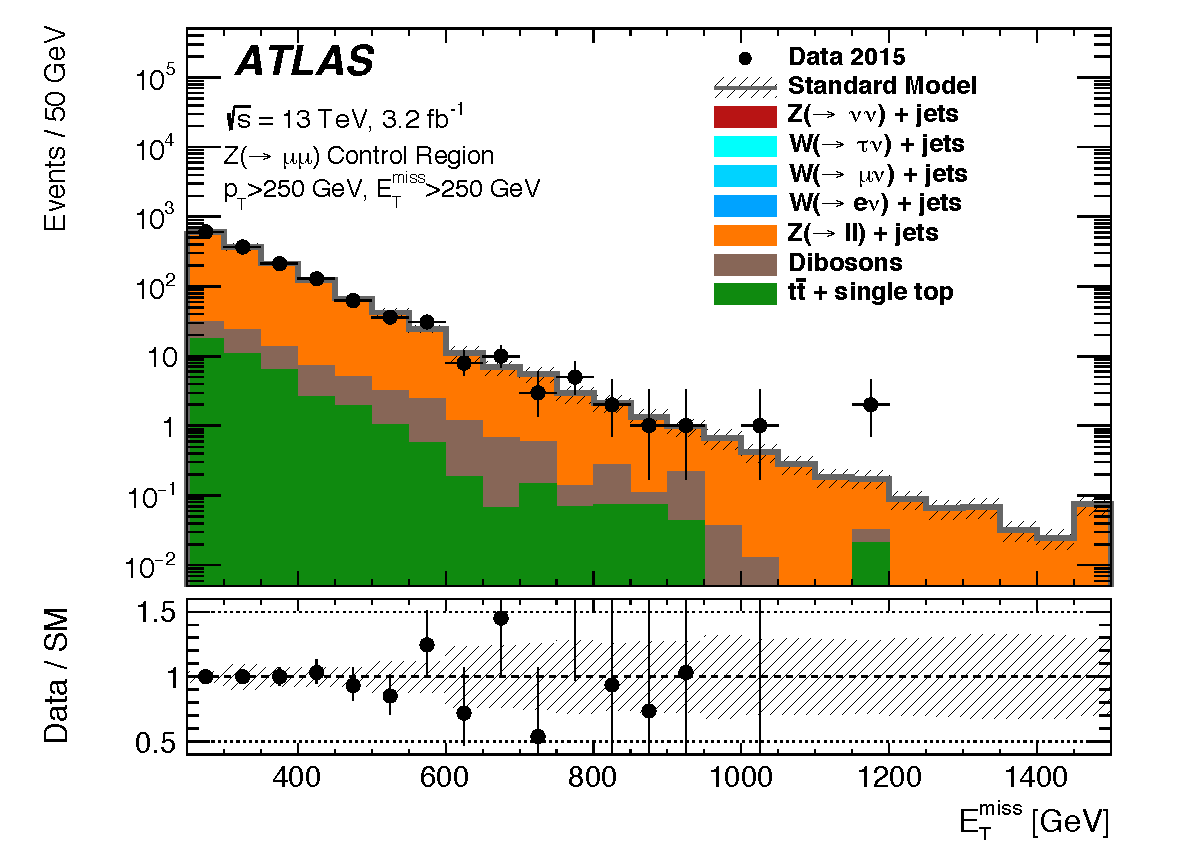
\includegraphics[width=\linewidth]{dimuon_cr_et_miss_post_fit}
    \caption{$\met$ distribution.}
    \label{fig:dimuon_cr_et_miss_pre_fit}
  \end{subfigure}
  \begin{subfigure}[t]{.48\linewidth}
    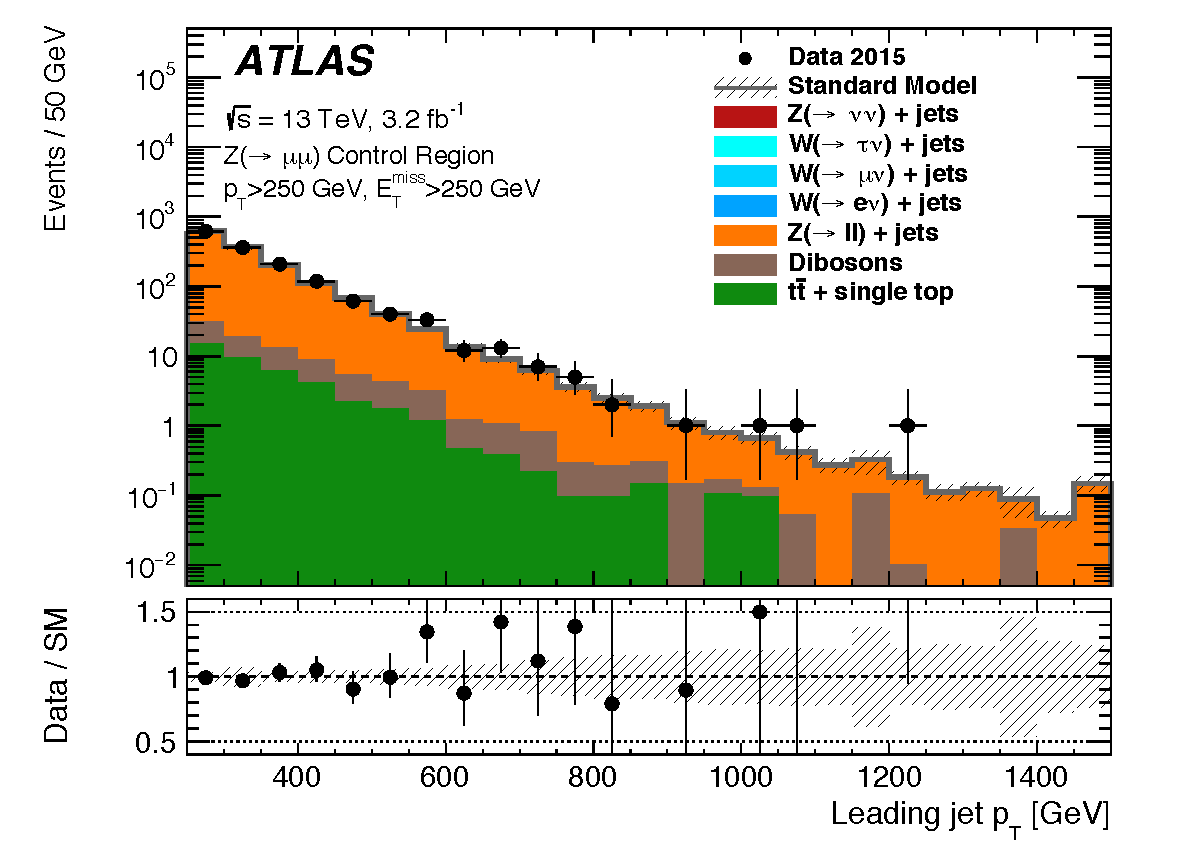
\includegraphics[width=\linewidth]{dimuon_cr_jet1_pt_post_fit}
    \caption{Leading jet $\pt$ distribution.}
    \label{fig:dimuon_cr_jet1_pt_pre_fit}
  \end{subfigure}
  \caption{Observed and predicted $\met$ and leading jet $\pt$ distributions
    after the background only fit in the di--muon $\crzmm$ for the
    $\met > 250~$GeV selection. The error bands include the statistical and
    systematic error.}
  \label{fig:dimuon_cr_plots}
\end{figure}
%%% Local Variables:
%%% mode: latex
%%% TeX-master: "../search_for_DM_LED_with_ATLAS"
%%% End:


\subsection{The Global Simultaneous Likelihood Fit}
\label{sec:glob-simult-likel}

A pure \gls{mc} based prediction of the \gls{bg} contamination in the signal
region yield large theoretical and experimental systematic uncertainties in the
shape and normalization of the predicted distributions. For this reason a data
driven approach, where the different backgrounds are normalized using the data
in \glspl{cr} that are orthogonal to the \gls{sr}, is used. To extrapolate from
\gls{cr} to \gls{sr} prediction a \emph{transfer factor} computed in \gls{mc} is
used. This factor is a ratio of \gls{mc} predictions in regions with similar
selections on missing transverse energy and jets thus most of the systematic
uncertainties either cancel out or are significantly reduced. The extrapolation
from one kinematic region to another can be itself a source of uncertainties.
To avoid this, the selection in terms of kinematic in the \glspl{cr} and
\glspl{sr} is chosen to be the same. The expected contributions of a background
process BG$_i$, which is extracted from a control region CR$_j$ to a signal
region SR$_k$, is given by:
\begin{equation}
  \label{eq:100}
  N_{\mathrm{\, BG}_i}^{\mathrm{\, SR}_k} = \frac{(N_\mathrm{\,
      data}^{\mathrm{\, CR}_j} - N_{\mathrm{\,
        non~BG}_i,~\mathrm{MC}}^{\mathrm{\, CR}_j})}
  {N^{\mathrm{\, CR}_j}_{\mathrm{\, BG}_i \mathrm{,~MC}}} \times
  N^{\mathrm{\, SR}_k}_{\mathrm{\, BG}_i,~\mathrm{MC}}
\end{equation}
where $N_{\mathrm{\, BG}_i}^{\mathrm{\, SR}_k}$ is the control region driven
predicted number events for background $i$ events in the signal region SR$_k$,
$N_\mathrm{\, data}^{\mathrm{\, CR}_j}$ is the observed number of events in the
control region $j$, $N_{\mathrm{\, non~BG}_i,~\mathrm{MC}}^{\mathrm{\, CR}_j}$
is the estimated number of the background contamination coming from other
processes in the given control region,
$N^{\mathrm{\, CR}_j}_{\mathrm{\, BG}_i \mathrm{,~MC}}$ is the \gls{mc}
prediction of the background $i$ in the control region $j$ and
$N^{\mathrm{\, SR}_k}_{\mathrm{\, BG}_i,~\mathrm{MC}}$ is the number of the
background $i$ events predicted in \gls{mc} simulation in the signal region. The
ratio:
\begin{equation}
  \label{eq:101}
  C_{\mathrm{BG}_i}^{\mathrm{CR}_j \rightarrow \mathrm{SR}_k} = \frac{
    N^{\mathrm{\, SR}_k}_{\mathrm{\, BG}_i,~\mathrm{MC}}}{N^{\mathrm{\,
        CR}_j}_{\mathrm{\, BG}_i \mathrm{,~MC}}}
\end{equation}
is the transfer factor used to extrapolate from CR$_j$ to SR$_k$. The factors
used in the normalization of the background expectation in the \glspl{sr} are
bin dependent and given by:
\begin{equation}
  \label{eq:102}
  \mu_{j} = \frac{(N_\mathrm{\, data}^{\mathrm{\, CR}_j} - N_{\mathrm{\,
        non~BG}_i,~\mathrm{MC}}^{\mathrm{\, CR}_j})}{N^{\mathrm{\,
        CR}_j}_{\mathrm{\, BG}_i \mathrm{,~MC}}}.
\end{equation}
The different normalization factors are not independent since different
processes can enter several CRs and thus the background subtraction term,
$N_{\mathrm{\, non~BG}_i,~\mathrm{MC}}^{\mathrm{\, CR}_j}$, gets contributions
from the other normalization factors. To properly treat the correlations, the
normalization factors are obtained from a simultaneous fit of all the CRs
referred to as the \emph{global fit}. A summary of the different processes and
the corresponding \gls{cr} used to extract the normalization factor is given in
\cref{tab:norm_factors}.

The global fit can be performed in two different ways:
\begin{enumerate}
\item The background only hypothesis, fits only the control regions in order to
  predict the background in the signal region. This fit is used to set model
  independent limits.
\item The signal plus background hypothesis, fits both the signal and control
  regions with a sum of background and specific signal. The normalization of the
  specific \gls{bsm} signal is a free parameter. This fit is used to exclude
  specific models.
\end{enumerate}
\begin{table}[!th]
  \centering
  \resizebox{\linewidth}{!}{\begin{tabular}{lll}
    \toprule
    Control Region & Background Process & Normalization Factor \\
    \midrule \midrule
    CR$_\mathrm{\, wmn}$ & $W (\rightarrow \mu \nu),\, Z (\rightarrow \nu \bar{\nu})$ & $\mu_\mathrm{\, wmn}$ \\
    CR$_\mathrm{\, ele}$ & $W (\rightarrow e \nu),\, W (\rightarrow \tau \nu),\,
                           Z/\gamma^* (\rightarrow \tau^+ \tau^-)$ & $\mu_\mathrm{\, ele}$ \\
    CR$_\mathrm{\, zmm}$ & $Z/\gamma^* (\rightarrow \mu^+ \mu^-)$ & $\mu_\mathrm{\, zmm}$ \\
    \bottomrule
  \end{tabular}}
  \caption{Summary table of the different background processes and the
    corresponding control regions used to evaluate the bin dependent
    normalization factors.}
  \label{tab:norm_factors}
\end{table}

%%% Local Variables:
%%% mode: latex
%%% TeX-master: "../search_for_DM_LED_with_ATLAS"
%%% End:


\section{Other Backgrounds}
\label{sec:other-backgrounds}

\subsection{The Multi-Jet Background}
\label{sec:multi-jet-background}

The multi--jet background events are mainly due to mis--reconstruction or loss
in some dead part of the calorimeter of jets or to the presence of neutrinos in
some heavy--flavor hadronic decay. The acceptance in the SR for multi--jet
events is low, nevertheless the large cross section of this process could
potentially lead to a high contamination in the SR\@. The use of MC simulation
in order to estimate the contribution to BG of this process is very difficult
due to the very large MC samples that would be required and the detailed
modeling of any calorimeter defects. For these reasons a data--driven technique,
the \emph{jet smearing method}, is used. It addresses event topologies with
large $\met$ originating from jet mis-reconstruction. This method creates large
sample of well measured low $\met$ jets called \emph{seeds} which are
\emph{smeared} using a function that quantify the $\pt$ fluctuation of a
measured reconstructed jet (the \emph{response function}) to create $\met$ in
the event. This process is reiterated many times to create a \emph{pseudo-data}
sample that is used in the SR analysis selection to estimate the distribution of
variables defining the control and signal regions. The procedure is described in
more details in Ref.~\cite{JetSmearing}. The multi-jet control region is defined
by inverting the $\Delta \phi_\mathrm{\, min} (\met, \mathrm{jet})$ and applying
the inclusive and exclusive SR $\met$ cuts. For the EM1 and IM1 the multi-jet
background constitutes the 0.5\% of the total BG and it is negligible in other
signal regions.
% \begin{figure}[!h]
%   \centering
%   \begin{subfigure}[t]{.48\linewidth}
%     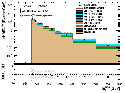
\includegraphics[width=\linewidth]{multijet_et_miss}
%     \caption{$\met$ distribution.}
%     \label{fig:dimuon_cr_et_miss_pre_fit}
%   \end{subfigure}
%   \begin{subfigure}[t]{.48\linewidth}
%     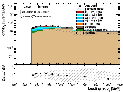
\includegraphics[width=\linewidth]{multijet_jet1_pt}
%     \caption{Leading jet $\pt$ distribution.}
%     \label{fig:dimuon_cr_jet1_pt_pre_fit}
%   \end{subfigure}
%   \caption{The $\met$ and the leading jet $\pt$ key variable distribution in the
%     multi-jet control region with $\pt > 250$~GeV and $\met > 250$~GeV.}
%   \label{fig:multijet_distributions}
% \end{figure}
%%% Local Variables:
%%% mode: latex
%%% TeX-master: "../search_for_DM_LED_with_ATLAS"
%%% End:


\subsection{The Non-Collision Background}
\label{sec:non-coll-backgr}

Non collision background is a term used to refer to BG processes coming from
cosmic particles, beam induced muons resulting from proton-gas inelastic
interaction or beam halo protons intercepting the LHC collimators and detector
noise. The characteristic signature of NCB is that of a jet recoiling against
invisible energy thus resembling the monojet final state signature. The jet
quality selection criteria mentioned in \cref{sec:event-selection} manage to
reduce the rate of jet coming from cosmic muons to a negligible amount compared
to the rate of data in the SR thus the main source of NCB is \gls{bib}. In order
to estimate the BIB contribution the two-sided no-time
method~\cite{BeamInducedBackground} was used. This method tries to match a
calorimeter energy cluster with a muon segment in both A and C side of the
detector. This topology corresponds to a particle moving parallel to the beam
line but several meters away from the beam axis and thus presumably arising from
beam background. An estimate of the number of NCB events in the SR is obtained
by correcting the number of events tagged as BIB inside the signal region for
the efficiency of the method. The efficiency of the tagger is estimated in a
sample of events in the SR failing the jet tight cleaning criteria that is
dominated by BIB jets.

The NCB contribution in the IM1 results in $112 \pm 23$ events and only
$19 \pm 9$ events in the EM3, this constitutes about 0.5\% of the total
background in these regions. For $\met > 500~$GeV there is no NCB contribution
in the signal region.
%%% Local Variables:
%%% mode: latex
%%% TeX-master: "../search_for_DM_LED_with_ATLAS"
%%% End:


\section{Systematic Uncertainties}
\label{sec:syst-uncert}

Systematic uncertainties can originate from the theory, caused for example by
our limited knowledge of the parton distribution function, or from experimental
sources such as the absolute jet energy scale and resolution or production cross
section for various processes determination. The systematic uncertainties are
treated as Gaussian nuisance parameters in the global likelihood fit described
in \cref{sec:glob-simult-likel}.
%%% Local Variables:
%%% mode: latex
%%% TeX-master: "../search_for_DM_LED_with_ATLAS"
%%% End:


\subsection{Theoretical Uncertainties}
\label{sec:theor-uncert}

The normalization factor for the $\znunuplusjets$ is constrained primarily from
the single muon control region. Following the run 1 analysis
strategy~\cite{RunIPaper}, a conservative 3\% uncertainty is used. It was
obtained by taking the maximum variation of the number of $\znunuplusjets$
events in bins of the leading jet $\pt$ and $\met$ predicted by
\textsc{sherpa}~\cite{SHERPA} and \textsc{alpgen}~\cite{ALPGEN}, with two
different parton showering algorithms. This 3\% uncertainty was therefore a
simple way to estimate generator uncertainty and parton shower uncertainty.

In addition an electroweak correction that takes into account the theoretical
differences between the $W$ and $Z$ bosons $\pt$ as described in
Ref.~\cite{EWCorrections} is added in quadrature to the flat 3\% introduced
earlier leading to a $\pm 3.5\%$ and $\pm 6\%$ uncertainty in the IM1 and IM7
region respectively.

\emph{Top quark} production processes get their uncertainties from the
$t \bar{t}$ and single-top production cross section, levels of initial and final
state radiation, the model used to generate the parton shower. This introduces a
$\pm 2.7\%$ and $\pm 3.3 \%$ variation in the top background estimation in the
IM1 and IM7 signal region respectively.

Uncertainties coming from \emph{diboson} processes are estimated using different
\gls{mc} generators and account for an uncertainty between $\pm 0.05\%$ and
$\pm 0.4$ on the number of events in the signal region.
%%% Local Variables:
%%% mode: latex
%%% TeX-master: "../search_for_DM_LED_with_ATLAS"
%%% End:


\subsection{Experimental Uncertainties}
\label{sec:exper-uncert}

Experimental systematic uncertainties can be divided in the following broad
categories:
\begin{itemize}
\item \textbf{Jet/$\met$}: This category includes uncertainties on the $\met$
  and jet energy scale and resolution, jet quality, pile-up estimation and
  $\pt$ measurement.
\item \textbf{Leptons}: This category includes uncertainties related to the
  identification, simulation, reconstruction efficiencies and energy and
  momentum resolution of electrons and muons.
\item \textbf{Luminosity}: Is the uncertainty on the integrated luminosity.
\end{itemize}
A $\pm 5\%$ uncertainty is assigned to the \emph{integrated luminosity}. Since
the efficiency plateau of the HLT\_xe70 is reached below 250~GeV $\met$ values,
no uncertainty is assigned to the trigger. Uncertainties in the jet and $\met$
\emph{energy scale} and \emph{resolution} contribute to the total background
with a variation of the number of predicted events of $\pm 0.5\%$ and
$\pm 1.6\%$ in the IM1 and IM7 respectively. The jet quality requirement,
pile-up estimation and correction to the measured $\met$ and jet $\pt$ results
in an uncertainty in the estimation of the total background of $\pm 0.2\%$ in
the IM1 and $\pm 0.9 \%$ in the IM7 control region. Lepton \emph{identification}
simulation and \emph{reconstruction efficiency} lead to a $\pm 0.1\%$
uncertainty in the IM1 and IM7 regions while energy and momentum
\emph{resolution} results in a $\pm 1.4\%$ variation in the IM1 selection and a
$\pm 2.6\%$ uncertainty in the IM7 signal region. A flat $\pm 100\%$ uncertainty
is assigned to \emph{multi-jet} and \emph{NCB} that translates to a $\pm 0.2\%$
variation in the total background in the IM1 signal region.
%%% Local Variables:
%%% mode: latex
%%% TeX-master: "../search_for_DM_LED_with_ATLAS"
%%% End:


\section{Results and Interpretations}
\label{sec:results}

The number of events observed in data in the signal regions was compared with
the background only fit. The results of the comparison between the observed
number of events in data and the background calculations including the
background only fit is shown in \cref{fig:sr_plots}. No significant excess of
data over background is observed. The results of the global fit procedure
described in Section~\ref{sec:glob-simult-likel} are used to set model
independent exclusion limit (see Section~\ref{sec:model-indep-limits}) and
interpreted in terms of squark pair production with
$\widetilde{q} \rightarrow q + \widetilde{\chi}_1^0\, (q = u,\, d,\, c,\, s)$
(see Section~\ref{sec:interpretation}).
\begin{figure}[!th]
  \centering
  \begin{subfigure}[t]{.48\linewidth}
    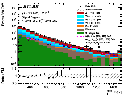
\includegraphics[width=\linewidth]{sr_et_miss}
    \caption{$\met$ distribution.}
    \label{fig:sr_et_miss}
  \end{subfigure}
  \begin{subfigure}[t]{.48\linewidth}
    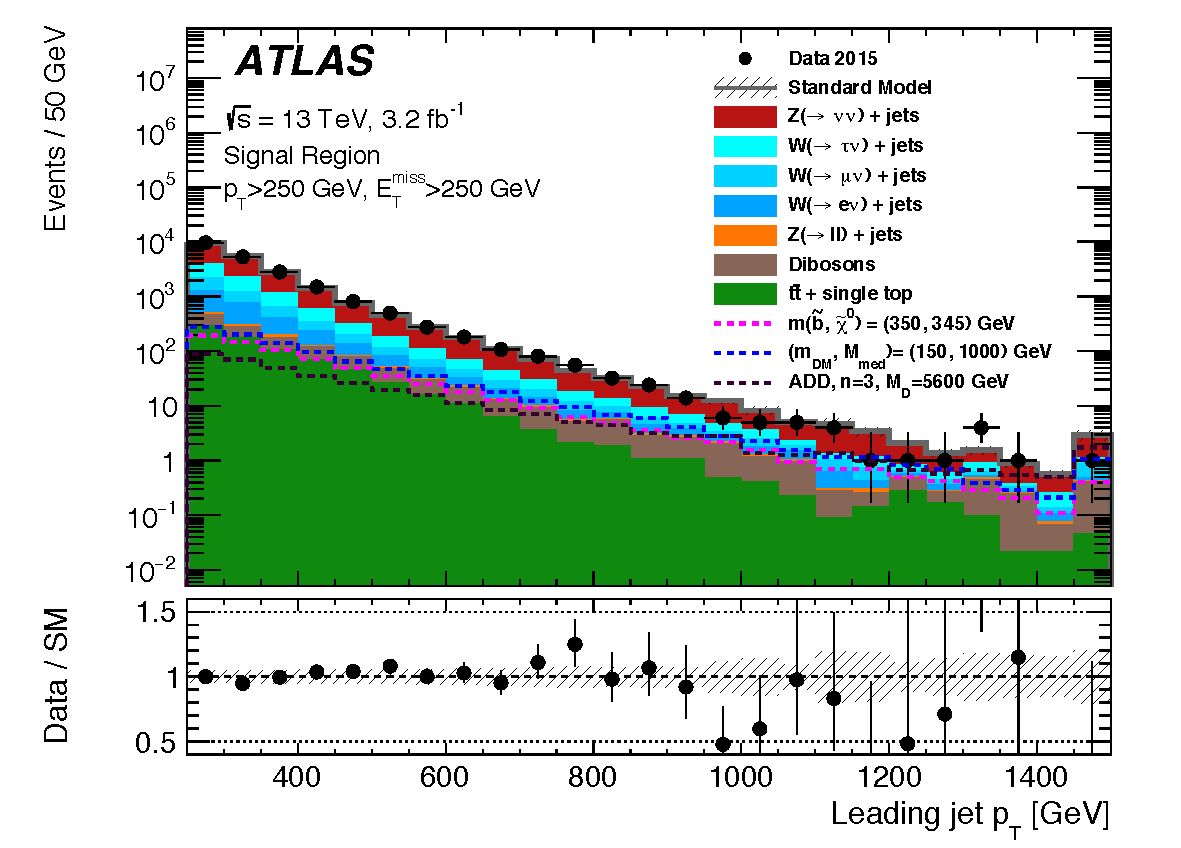
\includegraphics[width=\linewidth]{sr_jet1_pt}
    \caption{Leading jet $\pt$ distribution.}
    \label{fig:sr_jet1_pt}
  \end{subfigure}
  \caption{Distribution of the $\met$ and the leading jet $\pt$ for IM1 signal
    region compared with the background estimates from the background only fit
    in the control regions. The distributions of different signal models are
    superimposed for comparison. The contribution from the multi-jet and NCB
    background is negligible and not reported in the plot. In the ratio window
    the error bars include experimental and systematic uncertainties.}
  \label{fig:sr_plots}
\end{figure}
%%% Local Variables:
%%% mode: latex
%%% TeX-master: "../search_for_DM_LED_with_ATLAS"
%%% End:


% \subsection{The Signal Hypothesis Exclusion Procedure}
% \label{sec:sign-hypoth-excl}

% In general the physics search strategy for new phenomena can be outlined in four
steps, the first one is to define an \emph{hypothesis test}, the \emph{null
  hypothesis}, is that no signal is present i.e.~only known SM processes are
present in the SR and the \emph{alternate hypothesis} is that it exists. The
next steps are meant to quantify which one of the hypotheses is favored by
experimental observations. To this end it is necessary to identify the
observables of the experiment, next a \emph{test--statistic} (a function of
these observables) of the known background and to be tested signal is defined to
rank the experiments from the least to the most signal--like. Finally a rule to
quantify the significance of the exclusion or discovery is chosen.

In the monojet analysis the observable of the experiment is the number of events
in the signal regions defined with the criteria illustrated in
Section~\ref{sec:event-selection}, the CL$_\mathrm{\, S}$ described below is the
test--statistic and a \gls{cl} of 95\% is chosen for the exclusion. The number
of events observed in the signal region is governed by a Poisson distribution
\begin{equation}
  \label{eq:86}
  P(O|E) = \frac{E^O }{O!} e^{- E}
\end{equation}
where $O$ is the number of observed events and $E$ is the number of expected
events. In absence of signal (background only hypothesis), the expected number
of events is the total number of predicted background events from SM
processes. If some signal is present (signal plus background hypothesis), the
expected number of events is given by the predicted number of background events
plus the predicted number of signal events. In terms of Poisson distribution,
the probability of observing up to $N_\mathrm{\, SR}$ events in the SR in a
signal plus background hypothesis is:
\begin{equation}
  \label{eq:87}
  P(N_\mathrm{\, SR}|\mu_S + B) = \sum^{N_\mathrm{\, SR}}_{k = 0} \frac{(\mu_S + B)^k}{k!}
  e^{- (\mu_S + B)},
\end{equation}
where $\mu_S$ is the \emph{signal strength} and represents the number of
expected signal events. The lower this probability is, the more likely it is
that the tested signal is not present in the SR and the hypothesis of it
explaining some physics process can be excluded. To quantify the significance of
the exclusion a CL is calculated as:
\begin{equation}
  \label{eq:88}
  CL_\mathrm{\, S+B} = 1 - P(N_\mathrm{\, SR}|S+B) = 1 - \alpha
\end{equation}
where typically $\alpha = 0.05$ and a 95\% CL$_\mathrm{\, S+B}$ is quoted. The
maximum number of expected signal events (S$_\mathrm{\, max}$) for which
CL$_\mathrm{\, S+B}$ < 0.95 can be calculated and if the number of expected
signal events ($S$) exceeds this value (S > S$_\mathrm{\, max}$), the model can
be excluded~\cite{PawelThesis} with a confidence level $\alpha$. In the monojet
analysis the CL$_\mathrm{\, S}$ method~\cite{CLsMethod} is used, where:
\begin{equation}
  \label{eq:89}
  CL_\mathrm{\, S} = \frac{CL_\mathrm{\, S+B}}{CL_\mathrm{\, B}}.
\end{equation}
The CL$_\mathrm{\, S}$ method is preferred in high energy physics. It is
designed to address situations where the observed data could fluctuate below the
predicted SM background. This can happen in the case of low statistics, using
CL$_\mathrm{S + B}$ in this case can lead to exclude BSM signals even if the
experiment has no real sensitivity. The CL$_\mathrm{\, S}$ method allows to deal
with such situations and yields more conservative limits on the signal
hypothesis by normalizing the confidence level obtained in the signal plus
background hypothesis to the confidence level in the background only hypothesis.
%%% Local Variables:
%%% mode: latex
%%% TeX-master: "../search_for_DM_LED_with_ATLAS"
%%% End:


\subsection{The Statistical Procedure}
\label{sec:stat-proc}

The \emph{p-value} is the quantity used in the \gls{lhc} frequentist
approach~\cite{StatProcedure} to quantify the level of agreement between the
observed data and some hypothesis $H$. Assuming that $H$ is true, the p-value is
defined as the probability to observe data of equal or greater incompatibility
with $H$. In order to \emph{discover} a new physics signal, the \emph{null
  hypothesis}, $H_0$, is defined to include only known \gls{sm} processes
(background) and tested against an \emph{alternate hypothesis}, $H_1$, that
describes both the looked after signal and the background. If the signal cannot
be discovered the roles of the two hypotheses are inverted (the \emph{signal plus
  background} hypothesis becomes the null hypothesis and the \emph{background
  only} hypothesis becomes the alternate one) and \emph{exclusion limits} are
set instead. The conventionally accepted p-value to claim a discovery is set at
$2.87 \times 10^{-7}$ while to exclude a signal hypothesis a threshold p-value
of 0.005, often quoted as 95\%~\gls{cl}, is used.

In an experiment that measures a variable $x$ for each event in the signal
sample and constructs an histogram $\boldsymbol{n} = (n_1, \dots, n_N)$ out of
these measurements, the expectation value of $n_i$ can be written as:
\begin{equation}
  \label{eq:88}
  E[n_i] = \mu s_i + b_i
\end{equation}
where $s_i$ and $b_i$ are the mean number of signal and background entries in
the $i$-th bin and $\mu$ is the \emph{signal strength} parameter of the signal
process with $\mu = 0$ indicating the background only hypothesis and $\mu = 1$
the nominal signal one. The parameters of the physical model, unknown properties
of the response of the detector as well as other parameters that are not of
interest for the physics search are called \emph{nuisance parameters} and
indicated with $\boldsymbol{\theta}$. These can be evaluated constructing
histograms of some kinematic variable of interest in a control region where
mostly background events are expected. Indicating as
$\boldsymbol{m} = (m_1, \dots, m_M)$ one of such histograms, the expectation
value of the $i$-th bin, $m_i$, is given by:
\begin{equation}
  \label{eq:89}
  E[m_i] = u_i(\boldsymbol{\theta})
\end{equation}
where $u_i$ are calculable quantities that depend on the nuisance parameters
$\boldsymbol{\theta}$. With these definitions, the \emph{likelihood} function
can be written as the product of Poisson probabilities for the different bins:
\begin{equation}
  \label{eq:115}
  L(\mu, \boldsymbol{\theta}) = \prod_{j = 1}^N \frac{(\mu s_j +
    b_j)^{n_j}}{n_j!} e^{-(\mu s_j + b_j)} \prod_{k = 1}^M
  \frac{u_k^{m_k}}{m_k!} e^{-u_k}
\end{equation}

The p-value is determined at \gls{lhc} using the \emph{test
  statistics}~\cite{StatProcedure}:
\begin{equation}
  \label{eq:86}
  t_\mu = - 2 \ln \lambda(\mu)
\end{equation}
where $\lambda(\mu)$ is the \emph{profile likelihood ratio} defined as:
\begin{equation}
  \label{eq:87}
  \lambda(\mu) = \frac{L(\mu, \hat{\hat{\boldsymbol{\theta}}})}{L(\hat{\mu},
    \hat{\boldsymbol{\theta}})}.
\end{equation}
Here $\hat{\mu}$ and $\hat{\boldsymbol{\theta}}$ are the maximum likelihood
estimators, $L(\hat{\mu}, \hat{\boldsymbol{\theta}})$ is the maximized likelihood
function and $\hat{\hat{\boldsymbol{\theta}}}$ is the value of the parameters
$\boldsymbol{\theta}$ that maximizes the likelihood for a fixed value of the
signal strength $\mu$.
%%% Local Variables:
%%% mode: latex
%%% TeX-master: "../search_for_DM_LED_with_ATLAS"
%%% End:


\subsubsection{The $\cls$ Method}
\label{sec:cls-method}

\begin{figure}[!h]
  \centering
  \begin{subfigure}{.48\linewidth}
    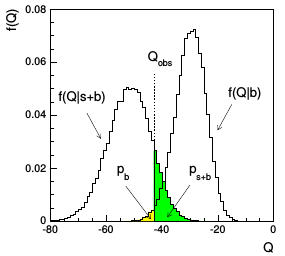
\includegraphics[width=\linewidth]{cls_ingredients}
    \caption{.}
  \end{subfigure}
  \begin{subfigure}{.48\linewidth}
    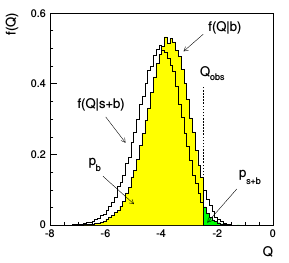
\includegraphics[width=\linewidth]{cls_underfluctuation}
    \caption{}
  \end{subfigure}
  \caption{~\cite{CowanCLsPlots}.}
  \label{fig:cls_method}
\end{figure}
%%% Local Variables:
%%% mode: latex
%%% TeX-master: "../search_for_DM_LED_with_ATLAS"
%%% End:


\subsection{Expected Limits}
\label{sec:expected-limits}

Since in the compressed \gls{susy} squark-neutralino model the $\met$ and jets
recoil against an \gls{isr} jet, the average jet momenta are lower than the
missing energy, thus requiring an asymmetric cut on the leading jet momentum and
$\met$ to capture this signal. Prior to deciding the signal region selections
presented in \cref{sec:event-selection} a signal region (AM1) with
$\met > 700$~GeV and leading jet $\pt > 300$~GeV was defined and compared with
the IM1 signal region. Since the final integrated luminosity cannot be known in
advance, the studies on AM1 and IM1 were carried out on a foreseen integrated
luminosity of L~=~3.3~$\ifb$. The results for these two signal regions is
presented in \cref{fig:im1_straight_comparison}. On these figure a model is
excludable if the signal strength $\mu$, depicted by the color scale in the
picture, is lower than one. The sensitivity improves for the signal region AM1
to reflect the asymmetric kinematics.

In the AM1 signal region, models with mass gaps $\Delta m = 5$~GeV between the
squark mass and the neutralino mass, can be excluded up to squark masses of
650~GeV. At a larger mass gap of $\Delta m = 25$~GeV, squark masses up to
580~GeV are excludable.

The performance of the shape fit method was also tested on the \gls{susy}
compressed squark-neutralino model and the result is also shown in
\cref{fig:im1_straight_comparison}. The shape fit method, thanks to its
flexibility, is capable of adapting to different signal models and thus improves
the expected limits of the SUSY squark-neutralino model especially for the
largest mass gap of $\Delta m = 25$~GeV between the squark and the neutralino
masses.
\begin{figure}[!htb]
  \centering
  \begin{subfigure}[t]{.48\linewidth}
    \includegraphics[width=\linewidth]{expected_im1}
    \caption{IM1.}
    \label{fig:expected_im1}
  \end{subfigure}
  \begin{subfigure}[t]{.48\linewidth}
    \includegraphics[width=\linewidth]{expected_straight_cut}
    \caption{AM1.}
    \label{fig:expected_straight}
  \end{subfigure}
  \begin{subfigure}[t]{.48\linewidth}
    \includegraphics[width=\linewidth]{expected_shape_fit}
    \caption{Shape fit.}
    \label{fig:expected_shape}
  \end{subfigure}
  \caption{Sensitivity to the compressed SUSY models with an integrated
    luminosity of L$~=~3.3~\ifb$~in the plane defined by the squark mass
    $m_{\tilde{q}}$ and the mass difference between the squark mass and the
    lightest neutralino mass
    $\Delta m = m(\tilde{q}) - m(\tilde{\chi}_{1}^{0})$. The color scale
    reflects the lowest excludable signal strength for a particular mass
    point. The values indicated on the map indicate the actual excludable $\mu$
    values at a some specific SUSY models. The dashed line shows the limit
    between excludable and not excludable models. The theoretical uncertainties
    in the signal are not included.}
  \label{fig:im1_straight_comparison}
\end{figure}
\pagebreak[4]
%%% Local Variables:
%%% mode: latex
%%% TeX-master: "../search_for_DM_LED_with_ATLAS"
%%% End:


\subsection{Model Independent Limits}
\label{sec:model-indep-limits}

The \emph{visible cross section} represents the number of BSM events in the
signal region in units of luminosity and is defined as:
\begin{equation}
  \label{eq:113}
  \sigma_\mathrm{\, vis} = \sigma \times A \times \epsilon
\end{equation}
where $\sigma$ is the production cross section, $A$ is the selection acceptance
and $\epsilon$ is the selection efficiency. The CL$_\mathrm{\, S}$ modified
frequentist approach introduced in \cref{sec:cls-method} is used to
set 95\% CL exclusion limit on the \emph{visible cross section} for models with
a monojet final state experimental signature. The results are reported in
\cref{tab:cs_vis_results}, values of $\sigma_\mathrm{\, vis}$ above
$\langle \sigma \rangle_\mathrm{\, obs}^{\, 95}$ are excluded at 95\%
CL\@. These results can be understood as follow: BSM models with more than 19
events per inverse femtobarn of integrated luminosity in the IM7 signal region
are excluded by the ATLAS data.
\begin{table}[!h]
  \centering
  \begin{tabular}{llll}
    \toprule
    \multicolumn{4}{c}{Result Table} \\
    \midrule \midrule
    Signal Region & $\langle \sigma \rangle_\mathrm{\, obs}^{\, 95}$ [fb] & S$_\mathrm{\, obs}^{\, 95}$ & S$_\mathrm{\, exp}^{\, 95}$ \\
    \midrule
    IM1 & 533 & 1773 & 1864$_{\, -548}^{\, +829}$ \\
    IM2 & 308 & 988 & 1178$_{\, -348}^{\, +541}$ \\
    IM3 & 196 & 630 & 694$_{\, -204}^{\, +308}$ \\
    IM4 & 153 & 491 & 401$_{\, -113}^{\, +168}$ \\
    IM5 & 61 & 196 & 164$_{\, -45}^{\, +63}$ \\
    IM6 & 23 & 75 & 84$_{\, -23}^{\, +32}$ \\
    IM7 & 19 & 61 & 48$_{\, -13}^{\, +18}$ \\
    \bottomrule
  \end{tabular}
  \caption{Results on the expected and observed upper limits on the number of
    events, S$_\mathrm{\, exp}^{\, 95}$ and S$_\mathrm{\, obs}^{\, 95}$
    respectively and on the visible cross section at 95\% CL.}
  \label{tab:cs_vis_results}
\end{table}
%%% Local Variables:
%%% mode: latex
%%% TeX-master: "../search_for_DM_LED_with_ATLAS"
%%% End:


\subsection{SUSY Compressed Spectra Interpretation}
\label{sec:interpretation}

The results of model independent limits are interpreted in terms of limits
computed for squark pair production with $\squarkprod$ in a SUSY compressed
scenario. The sensitivity to these models is estimated by performing a global
signal plus background fit that includes the $\crele$, $\crwmn$, $\crzmm$
control regions, the signal regions and all the systematic uncertainties. The
expected limits are derived with the same procedure but by replacing the data
with the background prediction.

Figure~\ref{fig:expected_observed} shows the result limits on the SUSY
compressed squark--neutralino model for the Run~II 2015 data. This is the result
of the shape fit with a luminosity of $3.2~\ifb$ with all theoretical signal
systematic uncertainties included in the observed and expected exclusion contour
and using the $\crele$, $\crwmn$, $\crzmm$ control regions. The theoretical
uncertainty on the signal cross section is used to derive the uncertainty on the
observed limit.

Models with a mass gap of $\Delta m = 5$~GeV between the squark and the
neutralino mass can be excluded up to squark masses of 608~GeV. For larger mass
gap of $\Delta m = 25$~GeV, squark masses up to 532~GeV are also excluded. The
results of this study are combined with the more general SUSY searches adding
sensitivity to the region close to the diagonal (dashed line) in
\cref{fig:susy_exclusion}.


\begin{figure}[!h]
  \centering
    \includegraphics[width=.8\linewidth]{expected_observed}
    \caption{Expected and observed limits on the SUSY compressed models using
      the Run~2 2015 data, in the plane defined by the squark mass on the
      $x$-axis and the mass difference between the squark and lightest
      neutralino mass on the $y$-axis. All experimental and theoretical
      systematic uncertainties are included.}
\label{fig:results:susy:compressed_observed}
    \label{fig:expected_observed}
\end{figure}
%%% Local Variables:
%%% mode: latex
%%% TeX-master: "../search_for_DM_LED_with_ATLAS"
%%% End:


\chapter{The 2016 Monojet Analysis}
\label{cha:2016-monoj-analys}

\section{Phenomenology of The ADD Model}
\label{sec:phen-add-model}

\cite{ADDPaper}
%%% Local Variables:
%%% mode: latex
%%% TeX-master: "../search_for_DM_LED_with_ATLAS"
%%% End:


\section{Validity of The Effective Field Theory}
\label{sec:valid-effect-field}

As mentioned in \cref{sec:arkani-hamed-dimop} in the \gls{add} model, the
fundamental scale of the gravitational interaction, $\md$, is brought down to
the electroweak scale ($\md \approx 1~$TeV). At these energies, due to the large
center of mass energy available at \gls{lhc}, the validity of the predictions of
the \gls{eft} become unreliable. For this reason two different sets of limits
have been calculated, one where the full cross section is used and the other
where it is weighted down by a factor $\md^4/\hat{s}^2$ for events where
$\hat{s} > \md^2$, where $\hat{s}$ is the center of mass energy of the
partons~\cite{LEDWeightFactor}.

% This is implemented in the analysis by first calculating the $\hat{s}$
% distribution for each \gls{sr}

\cref{fig:shat} shows the $\hat{s}$ distribution in the 700 < $\met$ < 800~GeV
region for the ADD n = 6 model. The straight line indicates the excluded $\md$
value before any weighting of the events, a part of the generated events are in
the region where $\hat{s} > \md^2$ where the effective field theory predictions
are expected to not be reliable. \cref{fig:vis_sigma_trunc} shows the visible
cross section as a function of the fundamental Plank scale $\md$ in the 700 <
$\met$ < 800~GeV region for the ADD n = 6 model. The solid line is the visible
cross section for all the $\hat{s}$, while in the dashed one a $\md^4/\hat{s}^2$
weighting factor is applied for events where $\hat{s} > \md^2$, it can be seen
that for $\md = 0$ all events get weighted down since $\hat{s} > \md^2 = 0$. The
horizontal line is an hypothesized typical exclusion limit on the visible cross
section and it is not used in the analysis. The intersection point between the
dashed line and the horizontal one, would represent the excluded value on
$\md$. The black square is the nominal $\md$ value of the generated sample.

\begin{figure}[!h]
  \centering
  \includegraphics[width=\linewidth]{plot_nD6_SR700}
  \caption{Generated $\hat{s}$ for the signal region where 700 < $\met$ <
    800~GeV for the ADD n = 6 model. A line indicating the value of the excluded
    value of $\md$ is also reported in the figure.}
  \label{fig:shat}
\end{figure}

\begin{figure}[!h]
  \includegraphics[width=\linewidth]{plot_sigma_visible_nD6_SR700}
  \caption{Visible cross section as a function of $\md$ for the signal region
    where 700 < $\met$ < 800~GeV for the ADD n = 6 model. The solid line is the
    visible cross section for all the $\hat{s}$, while in the dashed one a
    $\md^4/\hat{s}^2$ weighting factor is applied for events where
    $\hat{s} > \md^2$. The horizontal line is the upper limit on the production
    cross section if only this region would be considered in the fit. The black
    square is the nominal $\md$ value of the generated sample.}
  \label{fig:vis_sigma_trunc}
\end{figure}
%%% Local Variables:
%%% mode: latex
%%% TeX-master: "../search_for_DM_LED_with_ATLAS"
%%% End:


\section{Signal Theroetical Systematic Uncertainties}
\label{sec:ther-syst-uncert}

The theoretical uncertainties associated to the ADD signal derive from the
uncertainties on the parton distribution function, the renormalization and
factorization scales, the tuning of the parton shower in
Pythia~\cite{PythiaManual} and the initial and final state radiation
modeling. The estimation of the theoretical uncertainties is outlined in the
following sections.
%%% Local Variables:
%%% mode: latex
%%% TeX-master: "../search_for_DM_LED_with_ATLAS"
%%% End:


\subsection{Parton Distribution Function Uncertainties}
\label{sec:pdf-uncertainties}

For precision measurement of the physics processes at the LHC, an accurate
description of the \gls{pdf} is important. The parton distribution functions are
non-perturbative and extracted from global fit to hard-scatter data. Two kind of
PDFs are considered:
\begin{itemize}
\item Intra-\gls{pdf} uncertainty: This is the uncertainty within a specific \gls{pdf}
  set.
\item Inter-\gls{pdf} uncertainty: This is the uncertainty when a certain
  \gls{pdf} is replaced with another.
\end{itemize}
Three different groups provide equally precise parton distribution functions
making it arbitrary to use one over the others to generate the signal MC
samples. For this reason the recommendation of the PDF4LHC~\cite{PDF4LHC} group
for a correct estimation of the \gls{pdf} uncertainty is to combine the
uncertainties from all three groups and thus the CT10~\cite{CT10}, the
NNPDF~\cite{NNPDF} and the MMHT~\cite{MMHT} \gls{pdf} sets have been used.

The MC signal samples for the \gls{add} model are generated using the NNPDF set,
in principle in order to evaluate the \gls{pdf} uncertainties for CT10 and MMHT
it would be necessary to re-generate the signal samples using these \gls{pdf}
sets. It is common practice to instead re-weight each event in the original
sample to the value it would have if it were generated using an alternate PDF
set. This is done using the LHAPDF~\cite{LHAPDF} tool.
% The weight is given by:
% \begin{equation}
%   \label{eq:63}
%   w = \frac{\mathrm{PDF}(x_1, f_1, Q) \cdot \mathrm{PDF}(x_2, f_2, Q)}
%   {\mathrm{PDF}_0(x_1, f_1, Q) \cdot \mathrm{PDF}_0(x_2, f_2, Q)}
% \end{equation}
% where $\mathrm{PDF}$ is the alternate \gls{pdf} and $\mathrm{PDF}_0$ is the
% \gls{pdf} used to generate the samples.

The CT10 and the MMHT sets provide error sets to estimate the intra-\gls{pdf}
uncertainty. The idea is that each \gls{pdf} has a number of uncorrelated
parameters that can be varied independently by $\pm 1\sigma$ and a new \gls{pdf}
can be calculated. This procedure is then repeated for each parameter in the
\gls{pdf} set resulting in a set of \glspl{pdf}. This procedure is also done
using the LHAPDF tool. The Hessian~\cite{Hessian} method is then used to
estimate the uncertainty on the sets of \glspl{pdf}.

For CT10 the symmetric Hessian method with 52 error sets is used where the
uncertainty is given by:
\begin{equation}
  \label{eq:74}
  \delta X = \sqrt{\sum_{k = 1}^{n_\mathrm{err}} \left(X^{(k)} -
      X^{(0)} \right)^2}
\end{equation}
where $X^{(0)}$ is the number of events using the best \gls{pdf} fit and
$X^{(k)}$ is the number of events using the \gls{pdf} calculated varying the
$k$-th parameter.

For MMHT the asymmetric Hessian method with 50 error sets is used and the
uncertainty is given by:
\begin{align}
  \label{eq:75}
    \delta x^{\mathrm{up}} & = \sqrt{\sum_{k = 1}^{n_\mathrm{err}/2}
      \mathrm{max}(0, X_{2k} - X_0, X_{2k - 1} - X_0)^2} \\
    \delta x^{\mathrm{down}} & = \sqrt{\sum_{k = 1}^{n_\mathrm{err}/2}
      \mathrm{max}(0, X_0 - X_{2k}, X_0 - X_{2k - 1})^2}
\end{align}
where $X_0$ is the number of events obtained with the best fit and $X_{2k}
(X_{2k -1})$ is the number of events calculated with the $2k$-th ($2k -1$-th)
parameter variation.

The NNPDF provides an ensemble of 100 \glspl{pdf} where the best value is given
by the mean and the uncertainty by the standard deviation.

Figure~\ref{fig:pdf_syst} presents the results in terms of signal yields for the
cross section as a function of the PDF family and its uncertainty source. It
shows the inter-\gls{pdf} and intra-\gls{pdf} uncertainties of the three
families. The final \gls{pdf} uncertainty is the envelope that contains the
error bands of the three families.
\begin{figure}[!h]
  \centering
  \begin{subfigure}{.48\linewidth}
    \includegraphics[width=\linewidth]{add_d2_MCut0_pdfset}
    \caption{ADD n = 2}
    \label{fig:}
  \end{subfigure}
  \begin{subfigure}{.48\linewidth}
    \includegraphics[width=\linewidth]{add_d3_MCut0_pdfset}
    \caption{ADD n = 3}
    \label{fig:}
  \end{subfigure}
  \begin{subfigure}{.48\linewidth}
    \includegraphics[width=\linewidth]{add_d4_MCut0_pdfset}
    \caption{ADD n = 4}
    \label{fig:}
  \end{subfigure}
  \begin{subfigure}{.48\linewidth}
    \includegraphics[width=\linewidth]{add_d5_MCut0_pdfset}
    \caption{ADD n = 5}
    \label{fig:}
  \end{subfigure}
  \begin{subfigure}{.48\linewidth}
    \includegraphics[width=\linewidth]{add_d6_MCut0_pdfset}
    \caption{ADD n = 6}
    \label{fig:}
  \end{subfigure}
  \caption{Systematic uncertainty from choice of the PDF set. The event yield
    before any selection from three different PDF families are compared. The
    final uncertainty on the cross section is the envelop that contains all
    three families with their error bands. The same procedure is also applied to
    the acceptances}
  \label{fig:pdf_syst}
\end{figure}

The PDF uncertainties affects both the overall ADD signal normalization or cross
section and the signal acceptance (the potential number of events registered by
the detector for a generated signal). These uncertainties are collected in
Table~\ref{tab:add_pdf_2016}.
\begin{table}[!ht]
  \centering
  \resizebox{\linewidth}{!}{
  \begin{tabular}{lccccc}
    \toprule
    \multicolumn{6}{c}{PDF Uncertainty} \\
    \midrule \midrule
    \quad & ADD n = 2 & ADD n = 3 & ADD n = 4 & ADD n = 5 & ADD n = 6 \\
    $\Delta \sigma$ & 11 & 18 & 27 & 35 & 43 \\
    $\Delta A (250 < \met < 300)$ & 4 & 8 & 10 & 11 & 17 \\
    $\Delta A (300 < \met < 350)$ & 2 & 5 & 3 & 4 & 14 \\
    $\Delta A (350 < \met < 400)$ & 5 & 7 & 3 & 1 & 8 \\
    $\Delta A (400 < \met < 500)$ & 8 & 11 & 12 & 13 & 13 \\
    $\Delta A (500 < \met < 600)$ & 13 & 13 & 15 & 11 & 14 \\
    $\Delta A (600 < \met < 700)$ & 16 & 16 & 18 & 20 & 8 \\
    $\Delta A (700 < \met < 800)$ & 18 & 21 & 19 & 15 & 20 \\
    $\Delta A (800 < \met < 900)$ & 21 & 19 & 20 & 12 & 9 \\
    $\Delta A (900 < \met < 1000)$ & 20 & 22 & 21 & 15 & 19 \\
    $\Delta A (\met > 1000)$ & 32 & 26 & 28 & 30 & 26 \\
    \bottomrule
  \end{tabular}}
  \caption{Systematic uncertainties in \% on PDFs. The uncertainty is the envelop the
    contains the signal yields from the three PDF families, plus their error
    bands.}
  \label{tab:add_pdf_2016}
\end{table}

%%% Local Variables:
%%% mode: latex
%%% TeX-master: "../search_for_DM_LED_with_ATLAS"
%%% End:


\subsection{Initial and Final State Radiation Uncertainties}
\label{sec:tune-uncertainties}

\gls{mb} events are soft ($\pt < 2$~GeV) inelastic interactions which constitute
a significant fraction of the hadron-hadron collisions. Understanding \gls{mb}
processes is therefore important for precision measurements of hard scatter
interactions. Perturbative \gls{qcd} is commonly used to describe parton
interactions when possible and non-perturbative \gls{qcd} for low $\pt$
processes. The free parameters of these models (\emph{tune parameters}) need to
be tuned in the \gls{mc} generators in order to replicate experimental
data. These variation of these parameters may lead to different number of
generated events in the \gls{mc} samples and thus to uncertainty in the
acceptance. Five tune parameters have been varied in order to account for
uncertainties from:
\begin{itemize}
\item Underlying event effects.
\item Jet structure effects.
\item Aspects of the MC generation that provide extra jet production.
\end{itemize}
For each ADD model, ten systematic samples are produced and analyzed at the
truth level, the effect of the acceptance is evaluated in the different bins
used in the analysis. The final uncertainty in each bin is a common envelope
valid for the different extra dimensions models (from ADD n = 2 to ADD n = 6),
the results are summarized in Table~\ref{tab:add_tune_scale}.
\begin{table}[!ht]
  \centering
  \resizebox{\linewidth}{!}{\begin{tabular}{lcccccccccc}
    \toprule
    \multicolumn{10}{c}{Initial and Final State Radiation} \\
    \midrule \midrule
    $\met$~[GeV] & 250-300 & 300-350 & 350-400 & 400-500 & 500-600 & 600-700 &
                                                                               700-800
 & 800-900 & 900-1000 & 1000-3000 \\
    $\Delta A(\%)$ & 11 & 11 & 8 & 7 & 7 & 10 & 13 & 18 & 13 & 9 \\
    \bottomrule
  \end{tabular}}
  \caption{Tune initial and final state radiation uncertainties in \% on the
    acceptance of the different signal region $\met$ bins in the analysis. The
    final value is a common envelope valid for all the ADD models between n = 2
    and n = 6 dimensions.}
  \label{tab:add_tune_scale}
\end{table}
%%% Local Variables:
%%% mode: latex
%%% TeX-master: "../search_for_DM_LED_with_ATLAS"
%%% End:


\subsection{Renormalization and Factorization Scale Uncertainties}
\label{sec:renorm-fact-scale}

The renormalization and factorization scale uncertainties are obtained by
re-generating the signal MC samples varying the two scales by a factor of 2 and
0.5 respectively. The final uncertainty is the average of the up and down
variations. This source of uncertainty mostly affects the cross section and the
results are collected in Table~\ref{tab:add_fact_ren_scale}.
\begin{table}[!ht]
  \centering
  \begin{tabular}{lccccc}
    \toprule
    \multicolumn{6}{c}{Renorm./Fact. Scale Uncertainty} \\
    \midrule \midrule
    \quad & ADD n = 2 & ADD n = 3 & ADD n = 4 & ADD n = 5 & ADD n = 6 \\
    $\Delta \sigma$ & 23 & 27 & 30 & 33 & 36 \\
    \bottomrule
  \end{tabular}
  \caption{Systematic uncertainty in \% on the ADD signal normalization arising from
    the factorization and renormalization scales. The scales are varied up and
    down simultaneously, the final uncertainty is the average of these
    variations.}
  \label{tab:add_fact_ren_scale}
\end{table}
%%% Local Variables:
%%% mode: latex
%%% TeX-master: "../search_for_DM_LED_with_ATLAS"
%%% End:


\section{Results and Interpretations}
\label{sec:results-interpr}

\subsection{ADD Model Interpretation}
\label{sec:add-model-interpr}

The results of the model independent limits are interpreted in terms of limits
on the fundamental Plank scale in $4 + n$ dimensions (M$_\mathrm{\, D}$) in the
Large Extra Dimensions (LED) scenario proposed by Arkani-Hamed, Dimopoulos and
Dvali (ADD)~\cite{ADDPaper}. In this model, a number of compact extra
dimensions, where only the graviton field is allowed to propagate, are added to
the usual 4 (three spatial dimensions and time) thus effectively reducing the
strength of the gravitational interaction whose scale, M$_\mathrm{\, D}$, could
be at the TeV scale. The generation of the signal and interpretation of the
results follows what was done in the 2015 analysis without major
modifications. Figure~\ref{fig:add_observed} shows the expected and observed
limits at 95\% CL on M$_\mathrm{\, D}$ as a function of the large extra
dimensions $n$. The dashed blue line shows the expected limits using $36.1~\ifb$
with the $\pm 1~\sigma$ and $\pm 2 \sigma$ error bands (green and yellow band
respectively). The red solid line is the observed limit. The limits for
$3.2~\ifb$ are also reported for comparison. Values of M$_\mathrm{\, D}$ up to
7.75~TeV for n = 2 dimensions and 4.8~TeV for n = 6 dimensions are excluded at
95\%~CL improving previous results. The limits where a
M$^4_\mathrm{\, D} / \hat{s}^2$ weighting factor is applied to the visible cross
section for events with $\hat{s} > $ M$^2_\mathrm{\, D}$ (truncation) where
$\hat{s}$ is the center of mass energy of the interacting partons is also
reported in parentheses; the effect of the the truncation is only noticeable in
the ADD n = 6 model meaning that the analysis is probing values of
M$_\mathrm{\, D}$ where the effective theory can be trusted.
\begin{table}[!hb]
  \centering
  \begin{tabular}{lcc}
    \toprule
    \multicolumn{3}{c}{95\% CL Limits on M$_\mathrm{\, D}$
    [TeV]} \\
    \midrule \midrule \\
    ADD Model & Expected & Observed (damped) \\
    n = 2 & 9.27$^{+0.79}_{-0.96}$ & 7.75$^{+0.45}_{-0.55}$ (7.75) \B \\
    n = 3 & 7.13$^{+0.48}_{-0.59}$ & 6.22$^{+0.36}_{-0.47}$ (6.22) \T \B \\
    n = 4 & 6.09$^{+0.34}_{-0.43}$ & 5.49$^{+0.32}_{-0.45}$ (5.49) \T \B \\
    n = 5 & 5.55$^{+0.27}_{-0.32}$ & 5.11$^{+0.30}_{-0.46}$ (5.11) \T \B \\
    n = 6 & 5.20$^{+0.22}_{-0.26}$ & 4.80$^{+0.26}_{-0.47}$ (4.78) \T \\
    \bottomrule
  \end{tabular}
  \caption{Expected and observed 95\% CL lower limits on the fundamental Plank
      scale M$_\mathrm{\, D}$ in $4 + n$ dimensions as a function of the number
      of extra dimensions $n$. The impact of the $\pm 1 \sigma$ uncertainty from
      the theory on the observed limits and the expected $\pm 1 \sigma$ range of
      limits in absence of a signal is reported. The 95\% CL observed limits
      after damping the signal cross section for $\hat{s} > M_D^2$ are also
      reported in parentheses.}
  \label{tab:add_limits}
\end{table}
\begin{figure}[!h]
  \centering
  \includegraphics[width=10cm]{add_exclusion_observed}
  \caption{Expected and observed limits at 95\% CL on the fundamental Planck
    Scale in $4 + n$ dimensions, M$_\mathrm{\, D}$, as a function of the number
    of extra dimensions $n$. The dashed blue line shows the expected limit using
    $36.5~\ifb$, the yellow band is the $\pm~1\sigma$ on the estimate. The solid
    red line is the observed limit with the suppression of the $\hat{s} >$
    M$_\mathrm{\, D}^2$ events (truncation) while the cyan line represents the
    observed limits in the 2015 analysis using $3.2~\ifb$.}
  \label{fig:add_observed}
\end{figure}
%%% Local Variables:
%%% mode: latex
%%% TeX-master: "../search_for_DM_LED_with_ATLAS"
%%% End:


\chapter{Conclusions}
\label{cha:conclusions}

The \gls{atlas} detector is a multipurpose detector used for precision
measurements of a wide range of Standard Model processes and in the search for
new decay channels of the Higgs boson and beyond the Standard Model phenomena
such as supersymmetry, extra dimensions or dark matter particles.

The Tile Calorimeter is the hadronic calorimeter covering the most central
region of the \gls{atlas} detector up to $|\eta| < 1.7$. It plays a vital role
in measuring the energy of jets and missing energy used in this thesis to search
for \gls{susy} and extra dimensions. To this end, an understanding of the
electronic noise inside the detector is crucial as it affects the signal left by
the particles crossing the calorimeter and must be known precisely. The exact
noise level per calorimeter cell is used as an input to the algorithm that
identifies significant calorimeter energy deposits and then identifies and
measure jets, electrons and taus. Part of the work presented in this thesis was
to update, monitor and study the noise calibration constants for the Tile
Calorimeter to allow for precise reprocessing of the 2011 data and the
identification of hadronic jets. During these studies unexpected variations over
time in the cell noise were observed. Further investigation led to discover that
the tile noise filter, an algorithm used to mitigate the effect of coherent
noise, was not behaving as expected in some situations significantly affecting
approximately 5\% of the cells in the TileCal.

This thesis presented two searches for \gls{bsm} physics in \gls{atlas}. The
first one used the 2015 data corresponding to an integrated luminosity of
3.2~$\ifb$ where for the first time the monojet analysis was used to set limits
on compressed light squark-neutralino models. Selections adapted to the specific
characteristics of this signal were studied. It was shown that the generic
approach provided by the global fit gives better sensitivity to this new signal
than a single signal region with asymmetric jet and $\met$ cuts. Several jet
veto criteria were considered since the \gls{bsm} compressed \gls{susy} scenario
studied in this thesis is the most sensitive to this type of cuts and considered
in the monojet analysis. No significant excess in the data compared to the
\gls{sm} predictions has been found thus the results have been translated into
model independent upper limits on the visible cross section with a 95\% \gls{cl}
and interpreted in terms of squark pair production with $\squarkprod$. Squark
masses up to 608~GeV are excluded. The study on the 2015 dataset extends limits
shown in \cref{fig:susy_exclusion} that are provided by the more classical
approach to \gls{susy} searches.

The second analysis presented in this thesis uses the combined 2015 + 2016
dataset corresponding to an integrated luminosity of 36.1~$\ifb$ which was used
to explore the presence of large extra dimensions in the \gls{add} model
scenario. A good agreement between data and Standard Model prediction is
observed and no significant excess in data is seen thus the results are
translated in 95\%~\gls{cl} upper limit on the effective Planck scale
$\md$. Values of $\md$ of 7.7 and 4.8~TeV for two and six extra dimension
hypotheses are excluded significantly improving the results obtained by the
previous version of the analysis.
% Naturalness suggests that supersymmetric standard model partners are expected at
% the TeV scale, with the high luminosity foreseen in 2016 it will be possible to
% test experimentally the squark pair production with masses at that scale.
%%% Local Variables:
%%% mode: latex
%%% TeX-master: "../search_for_DM_LED_with_ATLAS"
%%% End:


\printglossaries

\addcontentsline{toc}{chapter}{\bibname} \printbibliography
\end{document}
%%% Local Variables:
%%% mode: latex
%%% TeX-master: t
%%% End:
